\documentclass[a4paper, 12pt]{article} %oneside

\usepackage[utf8]{inputenc}
\usepackage[russian]{babel}
\usepackage{setspace}
\usepackage[left=30mm, top=20mm, right=15mm, bottom=20mm, nohead, footskip=10mm]{geometry} % настройки полей документа
\usepackage{lscape}
\usepackage{graphicx}
\usepackage{graphics}
\usepackage{subfigure}
\usepackage{indentfirst}
\usepackage[margin=10pt,font=small,labelfont=bf, labelsep=endash]{caption}
\usepackage{multirow}
\usepackage{amssymb}
\usepackage{amsmath}
\usepackage{xfrac}

\usepackage{siunitx}

\usepackage{stackengine}

% \usepackage{fancyhdr}
% \pagestyle{plain}

\usepackage{array}
\usepackage{makecell}

\usepackage{import}
\usepackage{example}

\usepackage{wrapfig}

\usepackage{hyperref}
\hypersetup{
    colorlinks,
    citecolor=black,
    filecolor=black,
    linkcolor=black,
    urlcolor=black
}

\usepackage{stackengine, amsmath, bm}

% tensor 2:
\newcommand{\tend}[1]{\hbox{\oalign{$\bm{#1}$\crcr\hidewidth$\scriptscriptstyle\bm{\sim}$\hidewidth}}}
%tensor 4:
\newcommand{\tenq}[1]{\hbox{\oalign{$\bm{#1}$\crcr\hidewidth$\scriptscriptstyle\bm{\approx}$\hidewidth}}}


\renewcommand\theadalign{bc}
\renewcommand\theadfont{\bfseries}
\renewcommand\theadgape{\Gape[4pt]}
\renewcommand\cellgape{\Gape[4pt]}
\newcommand\xrowht[2][0]{\addstackgap[.5\dimexpr#2\relax]{\vphantom{#1}}}

% Переносы математики.
\begingroup
\catcode`\+\active\gdef+{\mathchar8235\nobreak\discretionary{}{\usefont{OT1}{cmr}{m}{n}\char43}{}}
\catcode`\-\active\gdef-{\mathchar8704\nobreak\discretionary{}{\usefont{OMS}{cmsy}{m}{n}\char0}{}}
\catcode`\=\active\gdef={\mathchar12349\nobreak\discretionary{}{\usefont{OT1}{cmr}{m}{n}\char61}{}}
\catcode`\<\active\gdef<{\mathchar"313C\nobreak\discretionary{}{\usefont{OML}{cmm}{m}{n}\char60}{}}
\catcode`\>\active\gdef>{\mathchar"313E\nobreak\discretionary{}{\usefont{OML}{cmm}{m}{n}\char62}{}}
\endgroup
\def\times{\mathchar8706\nobreak\discretionary{}{\usefont{OMS}{cmsy}{m}{n}\char2}{}}
\def\subset{\mathchar"321A\nobreak\discretionary{}{\usefont{OMS}{cmsy}{m}{n}\char26}{}}
%\supset,\subseteq,\notin
\def\supset{\mathchar"321B\nobreak\discretionary{}{\usefont{OMS}{cmsy}{m}{n}\char27}{}}
\def\subseteq{\mathchar"3212\nobreak\discretionary{}{\usefont{OMS}{cmsy}{m}{n}\char18}{}}
\def\neq{\not=\nobreak\discretionary{}{\usefont{OMS}{cmsy}{m}{n}\char54\usefont{OT1}{cmr}{m}{n}\char61}{}}
\def\sim{\mathchar"3218\nobreak\discretionary{}{\usefont{OMS}{cmsy}{m}{n}\char24}{}}
\def\in{\mathchar"3232\nobreak\discretionary{}{\usefont{OMS}{cmsy}{m}{n}\char50}{}}
\def\to{\mathchar"3221\nobreak\discretionary{}{\usefont{OMS}{cmsy}{m}{n}\char33}{}}
\def\?#1{#1\nobreak\discretionary{}{\hbox{$\mathsurround=0pt #1$}}{}}
% Конец переносов математики.


\onehalfspacing
\sloppy
\hyphenpenalty=100000
\renewcommand{\thesubfigure}{(\asbuk{subfigure})}
\begin{document} % начало документа

% Восстанавливаем после amsmath.
\begingroup \catcode`\"=12
\gdef\newmcodes@{\mathcode`\'39\mathcode`\*42\mathcode`\."613A%
\mathcode`\-"8000\mathcode`\/47\mathcode`\:"603A\relax}%
\endgroup
\mathcode`\=="8000 \mathcode`\+="8000 \mathcode`\-="8000
\mathcode`\<="8000 \mathcode`\>="8000

\graphicspath{{images/}}

\title{Билеты к ГосЭкзамену \\ Физика материалов}
\date{25 мая 2023}

\maketitle

\pagebreak
\hspace{0pt}
\vfill
\begin{center}
    \textbf{Над написанием билетов работали:} \mbox{Беликова Д.Е.}, \mbox{Капелюшников А.С.}, \mbox{Каплина М.Д.}, \mbox{Карпов И.А.}, \mbox{Кирьянова А.В.}, \mbox{Крот А.Д.}, \mbox{Кузнецов К.М.}

    \textbf{Над оформлением работали:} \mbox{Капелюшников А.С.}, \mbox{Каплина М.Д.}, \mbox{Карпов И.А.}
\end{center}

\vfill
\hspace{0pt}
\pagebreak

\tableofcontents




\section{Колебания атомов одномерной двухатомной решетки. Акустические и оптические фононы, температура Дебая. Колебания атомов трехмерной 
решетки (зоны Бриллюэна, законы дисперсии и поверхности постоянной частоты).}

Рассмотрим одномерную решетку Бравэ с двумя ионами в элементарной ячейке, равновесные положения которых есть $na$ и $na+d$. Считаем, что оба иона идентичны, но что $d \leq a/2$, поэтому сила между соседними ионами зависит от того, равно ли это расстояние между ними $d$ или же $a-d$. 

\begin{figure}[h!]
    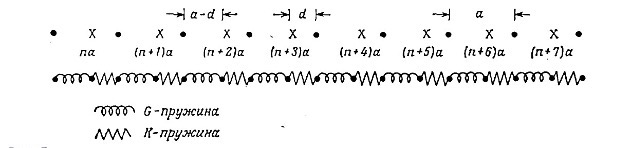
\includegraphics[width=\textwidth]{phys_1_1.png}
\end{figure}

Предположим, что взаимодействуют ближайшие соседи, причем сила взаимодействия больше для пар с расстоянием $d$, чем для пар с расстоянием $a-d$. Гармоническую потенциальную энергию можно представить в виде:

\begin{equation}
    U^{\text {harm }}=\frac{K}{2} \sum\left[u_1(n a)-u_2(n a)\right]^2+\frac{G}{2} \sum\left[u_2(n a)-u_1([n+1] a)\right]^2
\end{equation}

\noindent где через $u_1(na)$ обозначено смещение иона, совершающего колебания вблизи узла na, а через $u_2(na)$ --- смещение иона, колеблющегося вблизи узла na+d. Положим $K>=G$. Уравнения движения 

\begin{equation}
    \begin{aligned}
    M \ddot{u}_1(n a) & =-\frac{\partial U^{h a r m}}{\partial u_1(n a)}=-K\left[u_1(n a)-u_2(n a)\right]-G\left[u_1(n a)-u_2([n-1] a)\right] \\
    M \ddot{u_2}(n a) & =-\frac{\partial U^{h a r m}}{\partial u_2(n a)}=-K\left[u_2(n a)-u_1(n a)\right]-G\left[u_2(n a)-u_1([n+1] a)\right]
    \end{aligned}
\end{equation}


Ищем решение, представляющее собой волну с частотой $\omega$ и волновым вектором $k$: $u_1(n a)=\varepsilon_1 e^{i(k n a-\omega \mathrm{t})}$ и $u_2(n a)=\varepsilon_2 e^{i(k n a-\omega t)}$. Здесь $\epsilon_1$ и $\epsilon_2$ --- требующие определения постоянные, отношение которых дает относительные амплитуды и фазу колебаний ионов в каждой элементарной ячейке. Как и в моноатомном случае, периодическое граничное условие Борна-Кармана приводит к $N$ неэквивалентным значениям $k$. 

\begin{figure}[h!]
    \begin{center}
        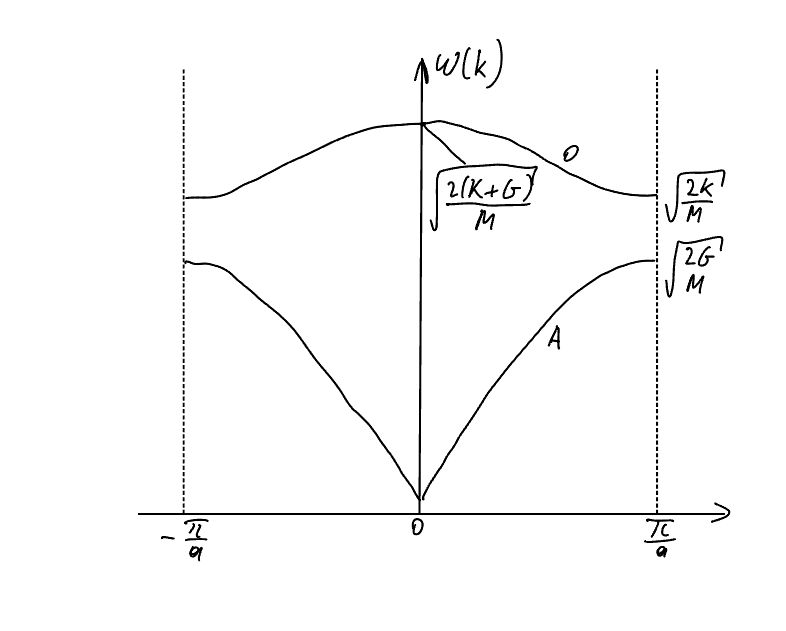
\includegraphics[width=0.7\textwidth]{phys_1_2}
    \end{center}
\end{figure}


\begin{equation}
    k=\frac{1\pi}{a} \frac{n}{N}
\end{equation}

Граничное условие (формулировка для линейной цепочки): соединяем два противоположных конца цепочки с помощью одной такой же <<пружинки>>, как и те, которые соединяют ионы внутри цепочки. 

Из полученных выше выражений получим 

\begin{equation}
    \begin{gathered}
    {\left[M \omega^2-(K+G)\right] \varepsilon_1+\left(K+G e^{-i k a}\right) \varepsilon_2=0} \\
    {\left[M \omega^2-(K+G)\right] \varepsilon_2+\left(K+G e^{i k a}\right) \varepsilon_1=0}
    \end{gathered}
\end{equation}

Данная пара уравнений имеет решение, если обращается в нуль детерминант, составленный из их коэффициентов, т.е. если выполняется условие 

\begin{equation}
    \left[M \omega^2-(K+G)\right]^2=\left|K+G e^{-i k a}\right|^2=K^2+G^2+2 K G \cos k a
\end{equation}

Данные уравнение выполняется для двух положительных значений $\omega$, для которых 

\begin{equation}
    \omega^2=\frac{K+G}{M} \pm \frac{1}{M} \sqrt{K^2+G^2+2 K G \cos k a}
\end{equation}
Причем $\displaystyle \frac{\varepsilon_1}{\varepsilon_2}=\mp \frac{K+G e^{-i k a}}{\left|K+G e^{-i k a}\right|}$

Для каждого из $N$ значений $k$ имеется, таким образом, 2 решения, что дает в целом $2N$ нормальных мод, ка и должно быть при $2N$ степенях свободы (по 2 иона в каждой из N элементарных ячеек). Две кривые зависимости $\omega$ от $k$ носят название 2 ветвей закона дисперсии.

Частота первой ветви $\omega$ пропорциональна $k$ при малых $k$, а на краях зоны Бриллюэна кривая становится почти горизонтальной. Эту ветвь называют акустической, так как ее закон дисперсии при малых $k$ имеет форму $\omega=ck$, характерную для звуковых волн. Вторая ветвь начинается при $k=0$ от значения  $\omega = \sqrt{2(K+G)/M}$ и опускается вниз с ростом $k$, достигая значения $\sqrt{2K/M}$ на границе зоны. Ее называют оптической ветвью, поскольку длинноволновые оптические моды в ионных кристаллах могут взаимодействовать с электромагнитным излучением. 

\textbf{Модель Дебая}

\begin{itemize}
    \item Колебания решетки рассматриваются как фононный газ
    \item Закон дисперсии фононов предполагается изотропным и линейным, то есть $\omega=u_sk$ ($u_s = const$)
    \item Первая зона Бриллюэна, которая представляет собой многогранник в пространстве волновых векторов, заменяется на шар того же объема. Его радиус $q_0$ находится из условия равенства объемов: $V_{\text{з.Бp.}}=\frac{4 \pi q_0^3}{3} \Rightarrow q_0=\left(\frac{6 \pi^2}{V_{\text {яч. }}}\right)^{1 / 3}$
    \item $0<\omega<\omega_{max}=\omega_D$
\end{itemize}

Для сплошной среды число состояний на элемент $dk$: 
\begin{equation}
    \frac{V 4 \pi k^3 d k}{(2 \pi)^3}
\end{equation}

При $\mathrm{T} \gg \Theta_{\mathrm{D}}$, где $\Theta_{\mathrm{D}}=\hbar \omega_{\mathrm{D}}$, температура Дебая, все осцилляторы допускают классическое описание.

$\mathrm{T} \ll \Theta_{\mathrm{D}}$, всегда найдутся осцилляторы, чье движение можно описывать классическими формулами, но остальные требуется описать квантово. 

\section{Спектральная плотность фононов. Модели Эйнштейна и Дебая. 
Теплоемкость кристаллической решетки.}

\textbf{Спектральная плотность колебаний решетки} (фононов) или плотность фононных состояний: $v(\omega)=\frac{1}{V} \frac{d N \omega}{d \omega}$, где $dN_\omega$ --- число фононных мод с частотами, лежащими в интервале ($\omega$; $\omega + d \omega$).

Спектральная плотность удовлетворяет условию нормировки $\displaystyle \int_0^{\infty} v(\omega) d \omega=\frac{3 N}{V_{\text {ячейки }}}$ (здесь $N$
--- число атомов в элементарной ячейке $3D$ кристалла, то есть $3N$ --- число степеней свободы). Зная законы дисперсии фононных ветвей, можно определить плотность фононных состояний как $\displaystyle v(\omega)=\sum_p \int \frac{d^3 \bar{k}}{(2 \pi)^2} \delta\left(\omega-\omega_p(\bar{k})\right)$, где $\delta(\omega)$ --- дельта-функция Дирака. Интеграл взят по первой зоне Бриллюэна. 

\begin{equation}
    \delta(\omega)=\left\{\begin{array}{c}
    +\infty, x=0 \\
    0, x \neq 0
    \end{array}\right.
\end{equation}

\textbf{Модель Эйнштейна}

\begin{itemize}
    \item Атомы в решетке ведут себя как $3N_a$ гармонических осцилляторов, не
    взаимодействуя друг с другом;
    Частота колебаний всех осцилляторов одинакова: $\omega_p(\bar{k})=\omega_E=const$. Модель качественно описывает оптические ветви, для которых $\omega_{\min}<\omega_p(\bar{k})<\omega_{\max}$, причем $\omega_{\min}$ и $\omega_{\max}$ --- величины одного порядка

    Для акустических ветвей модель Эйнштейна в области низких температур неприменима

    \item $\hbar \omega_p(\bar{k}) \geq T$. Так как $\omega_E=const$, $\nu(\omega)=3N\delta(\omega-\omega_E)$
\end{itemize}

\textit{Теплоемкость:}

Вычислим среднюю энергию осциллятора с частотой $\omega_i$ и полную энергию набора осцилляторов, так как фононы подчиняются статистике Бозе-Эйнштейна. 

\begin{equation}
    \bar{\varepsilon}_l=\frac{\hbar \omega_i}{e^{\hbar \omega_i / T}-1} ; \quad E_{\text {полн }}=\sum_{i=1}^{3 N} \frac{\hbar \omega_i}{e^{\hbar \omega_i / T}-1}
\end{equation}

Среднее число заполнения: $\langle n\rangle=\frac{1}{e^{\frac{\hbar \omega_i}{T}}-1}$

\begin{equation}
    E_{\text {полн }}=\int_0^{\omega_{\max }} \frac{\hbar \omega_i}{e^{\frac{\hbar \omega_i}{T}}-1} v(\omega) \mathrm{d} \omega = \int_0^{\omega_{\max }=\omega_E} \frac{\hbar \omega_i * 3 N}{e^{\frac{\hbar \omega_i}{T}}-1} \delta\left(\omega-\omega_E\right) \mathrm{d} \omega= \frac{\hbar \omega_E * 3 N}{e^{\hbar \omega_i / T}-1}
\end{equation}



\begin{equation}
    C_v=\frac{\partial E}{\partial T}=\frac{\hbar \omega_E \cdot 3 N-e^{\frac{\hbar \omega_E}{T}} \cdot \frac{\hbar \omega_E}{T^2}}{\left(e^{\frac{\hbar \omega_E}{T}}-1\right)^2}
\end{equation}


\textbf{Модель Дебая}

\begin{itemize}
    \item Колебания решетки рассматриваются как фононный газ.
    \item Закон дисперсии фононов предполагается изотропным и линейным, то есть $\omega = u_{s}k$, $(u_s=const)$.
    \item Первая зона Бриллюэна, которая представляет собой многогранник в пространстве волновых векторов, заменяется на шар того же объема. Его радиус $q_0$ находится из условия равенства объемов: $V_{\text{з.Бp.}}=\frac{4 \pi q_0^3}{3} \Rightarrow q_0=\left(\frac{6 \pi^2}{V_{\text {яч. }}}\right)^{1 / 3}$
    \item $0<\omega<\omega_{max}=\omega_D$
\end{itemize}

Для сплошной среды число состояний на элемент $dk=\frac{V 4 \pi k^3 d k}{(2 \pi)^3}$. Усредним $\omega=\overline{u_s}k$; $\frac{3}{\overline{u_{s}}^3} = \frac{1}{\overline{u_{e}}^3}+\frac{2}{\overline{u_{t}}^3}$, ($\omega_t=\overline{u_t}k$, $\omega_c=\overline{u_c}$ --- продольные и поперечные волны).
Тогда $\displaystyle \frac{V 4 \pi k^3 d k}{(2 \pi)^3} \rightarrow \frac{V 3 \omega^2 d \omega}{2 \pi^2 \bar{u}_s{ }^3} \rightarrow \nu(\omega)=\left\{\begin{array}{c}\frac{3}{2 \pi^2} \cdot \frac{\omega^2}{\overline{u_s}^3} \omega \leqslant \omega_D \\ 0, \quad \omega>\omega_D\end{array}\right.$

\textit{Теплоёмкость}

\begin{equation}
    C_v=\int_0^{\omega_D} \frac{(-1)  e^{\hbar \omega / T} \cdot \left(\frac{1}{T^2}\right) *(h \omega)^2}{\left(e^{\hbar \omega / T}-1\right)^2} v(\omega) d \omega,
\end{equation}

Новая переменная $\displaystyle \left\{\begin{array}{c}\varkappa=\frac{\hbar \omega}{T} \quad \mid \omega \rightarrow 0 \; \varkappa \rightarrow 0 \\ d \varkappa=\frac{\hbar}{T} d \omega \quad \mid \omega \rightarrow \omega_D \; \varkappa \rightarrow \frac{\Theta_D}{T}\end{array}\left(\Theta_D=\omega_D \hbar\right)\right.$

Тогда 
\begin{equation}
    \begin{aligned} & \left.C_v=\int_0^{\theta_D / T} \frac{e^\chi \chi^2}{\left(e^x-1\right)^2} * \frac{3 T^2 \varkappa^2}{2 \pi^2 \overline{u}_s{ }^2 \hbar^2} * \frac{T}{\hbar} d \varkappa=\frac{3 T^3}{2 \pi^2 \overline{u}^3 \mathrm{\hbar}^3} \int_0^{\theta_D / T} \frac{e^\chi \varkappa^4}{\left(e^x-1\right)^2}=\left( \begin{array}{l} \omega_D=\overline{u}_s k_D \\ \overline{u}_s=b\omega_D / k_D  \end{array}\right. \right) = \\ & =\frac{3}{2 \pi^2} *\left(\frac{T}{\theta_D}\right)^3 k_D{ }^3\left\{\begin{array}{c}T \ll \theta_D \Rightarrow \theta_D / T \rightarrow \infty \Rightarrow \int_0^{\infty} \varkappa^2 d \varkappa=\frac{4 \pi^2}{15} \\ T \gg \theta_D \Rightarrow \int_0^{\theta_D / T} e^{\varkappa} \varkappa^2 d \varkappa \approx \int_0^{\theta_D / T} \varkappa^2 d \varkappa=\frac{1}{3}\left(\frac{\theta_D}{T}\right)^3\end{array}\right. \\ & \end{aligned}
    \end{equation}
    
\begin{equation}
    C_v=\left\{\begin{array}{c}T \ll \theta_D \Rightarrow \frac{3}{2 \pi}\left(\frac{T}{\theta_D}\right)^3 k_D{ }^3 \frac{4}{15} \pi^2=\frac{2 \pi}{5}\left(\frac{T}{\theta_D}\right)^3 k_D{ }^3 \\ T \gg \theta_D \Rightarrow \frac{k_D{ }^3}{2 \pi} \Rightarrow\left\langle\int_0^{\omega_D} v(\omega) d \omega=3 N\right\rangle \Rightarrow \frac{3 N \pi^2}{2 \pi^2}=9 N\end{array}\right. 
\end{equation}


\section{Приближение почти свободных электронов. Поверхности Ферми металлов. Метод Харрисона.}

\begin{figure}[h!]
    \centering
    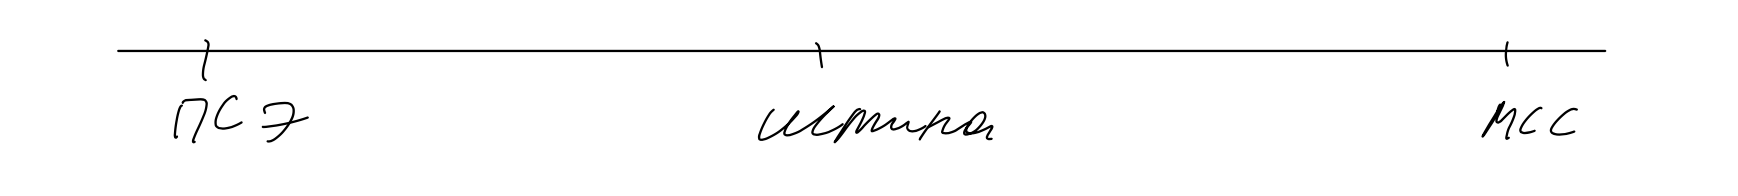
\includegraphics[width=0.8\textwidth]{phys_1_3.png}
\end{figure}

Применим для металлов; Электроны ведут себя почти как свободные; $U(r)$ мало 
(значительно меньше кинетической энергии); Используются методы теории возмущений 

Рассматривается движение электронов в линейной цепочке прямоугольных потенциальных ям шириной $a$, отделённых барьерами толщиной $b$ и высотой U0. Длина цепочки $L$, период $a+b$.
Решение уравнения Шрёдингера $\frac{\partial^2 \psi}{\partial x^2}+\frac{2 m}{\hbar^2}(E-U) \psi=0$ разбивается на две части

\begin{enumerate}
    \item $\mathrm{U}=0$, волновая функция представляется в виде $\psi_1(x)=A e^{i \alpha x}+B e^{-i \alpha x}$ (первое слагаемое - прямая волна, второе - отраженная от барьера)
    \item $\mathrm{U}=\mathrm{U}_0$, волновая функция: $\psi_2(x)=C e^{\beta x}+B e^{-\beta x}$.
    При этом $\alpha=\sqrt{\frac{2 m e}{\hbar^2}} \quad; \beta=\sqrt{\frac{2 m e\left(U_0-E\right)}{\hbar^2}}$.
\end{enumerate}

Подставляя в одномерную функцию Блоха $\psi(x)=U(x) \exp (i k x)$
$$
U_1(x)=A e^{(\alpha-i k) x}+B e^{-(\alpha+i k) x} ; \quad U_2(x)=C e^{(\beta-i k) x}+B e^{-(\beta+i k) x} .
$$
Oпределим A, B, C, D из непрерывности $U(x)$ и $U^{\prime}(x)$ в местах скачка потенциала. Т.е. для $\mathrm{x}=0$
$$
U_1(0)=U_2(0) ;\left(\frac{\partial U_1}{\partial x}\right)_{x=0}=\left(\frac{\partial U_2}{\partial x}\right)_{x=0}
$$ 

Также воспользуемся периодичностью $U(x): U_1(a)=U_2(-b) ;\left(\frac{\partial U_1}{\partial x}\right)_{x=a}=\left(\frac{\partial U_2}{\partial x}\right)_{x=-b}$

\begin{figure}[h!]
    \centering
    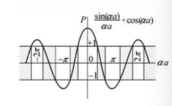
\includegraphics{phys_2_1}
\end{figure}


Подставляя в уравнения для $U_i(x)$, получим
$$
\frac{\beta^2-\alpha^2}{2 \alpha \beta} \mathrm{sh} (\beta b) \sin (\alpha a)+\mathrm{ch}(\beta b) \cos (\alpha a)=\cos k(a+b)
$$

Рассмотрим предельный случай $b \rightarrow 0, U_0 \rightarrow \infty$ при $b U_0= const =\frac{\hbar^2}{m a} P$. $\displaystyle P=\frac{m a}{h^2 b v_0}$ ($\mathrm{P}$ --- прозрачность барьера). Тогда: $\displaystyle P \frac{\sin (\alpha a)}{a d}+\cos (\alpha a)=\cos (k a) \text {. }$

Так как $-1<\cos<1$, левая часть уравнения от -1 до 1. Это и определяет область разрешённых состояний.

Таким образом, при построении зон Бриллюэна в приближении ПСЭ рассматривается чередование запрещенных и разрешенных зон. При этом

\begin{itemize}
    \item на границе $\displaystyle \frac{\partial E}{\partial k} =0$
    
    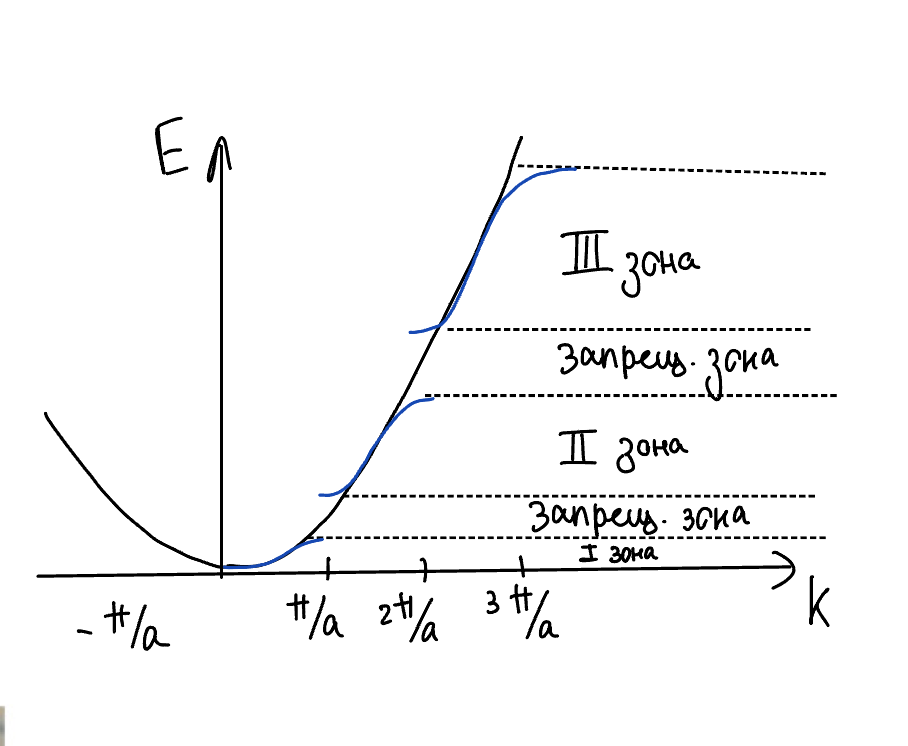
\includegraphics[width=0.4\textwidth]{phys_2_2} 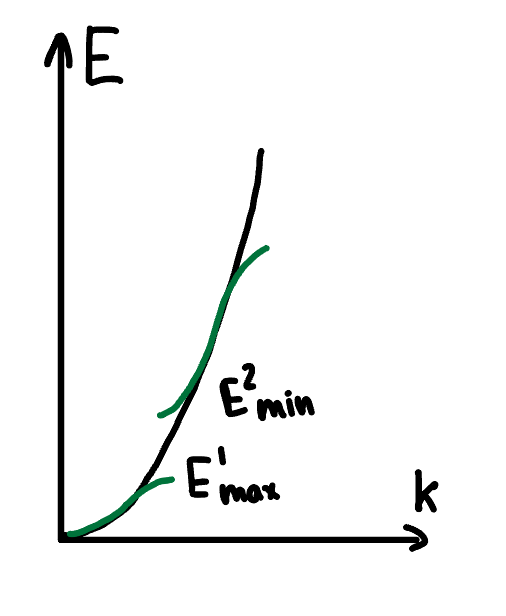
\includegraphics[width=0.2\textwidth]{phys_2_5}
    
    \item размеры зон одинаковы, поэтому число состояний в зонах конечно и одинаково
    \item в расширенной схеме каждая зона повторяется при трансляции на $\bar{a}$ : схема периодична, первая зона --- приведенная зонная схема 
\end{itemize}

\textbf{Заполнение зон Бриллюэна электронами в металлах:}

\begin{enumerate}
    \item Двухкомпонентная квадратичная решётка: 1-я зона --- куб (квадрат), 2-я зона --- призма (4 треугольника)
    \item $E_{\min} ^2 < E_{\max} ^1$ --- металлы Mg, Be (двухзонные). Проводимость: электронная по второй зоне, дырочная по первой (вторая зона заполняется после первой).
\end{enumerate}

\begin{figure}[h!]
    \centering
    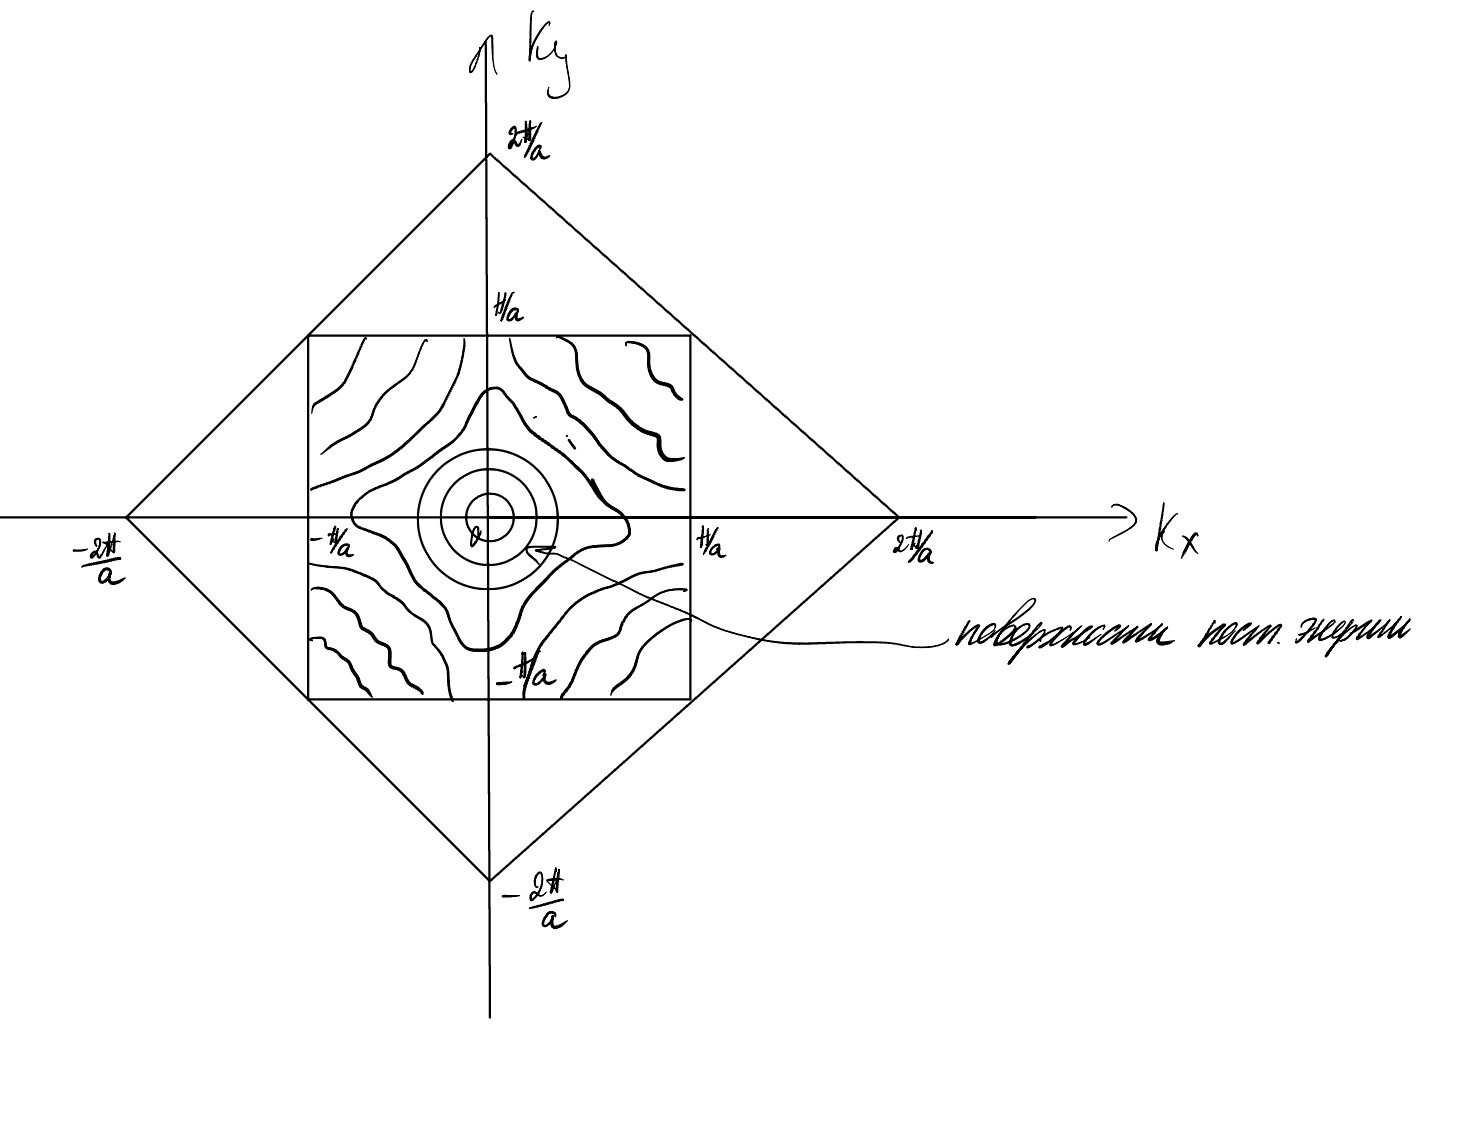
\includegraphics[width=0.5\textwidth]{phys_2_3}
\end{figure}



\textbf{Поверхность Ферми} --- поверхность с энергией Ферми, отделяющая пустые состояния от занятых.

\begin{itemize}
    \item Металлы 1-й группы. Na, Li, K, Au, Ag, Cu: первая зона заполнена на половину: $\displaystyle R^2 \pi=\frac{\pi^2}{2 a^2} \Rightarrow R^2=\frac{\pi}{2 a^2} \Rightarrow R=\frac{\pi}{a} \frac{1}{\sqrt{2 \pi}}$, $\displaystyle \mathrm{K}_{\mathrm{F}}=\frac{\pi}{a} \frac{1}{\sqrt{2 \pi}}$
    \item Металлы 2-й группы. Mg, Be, Zn, Cd: $R^2 \pi= \frac{4\pi^2}{a^2} \Rightarrow R^2=\frac{4 \pi}{a^2} \Rightarrow K_F=\frac{2 \sqrt{\pi}}{a}$

\end{itemize}

\begin{figure}[h!]
    \centering
    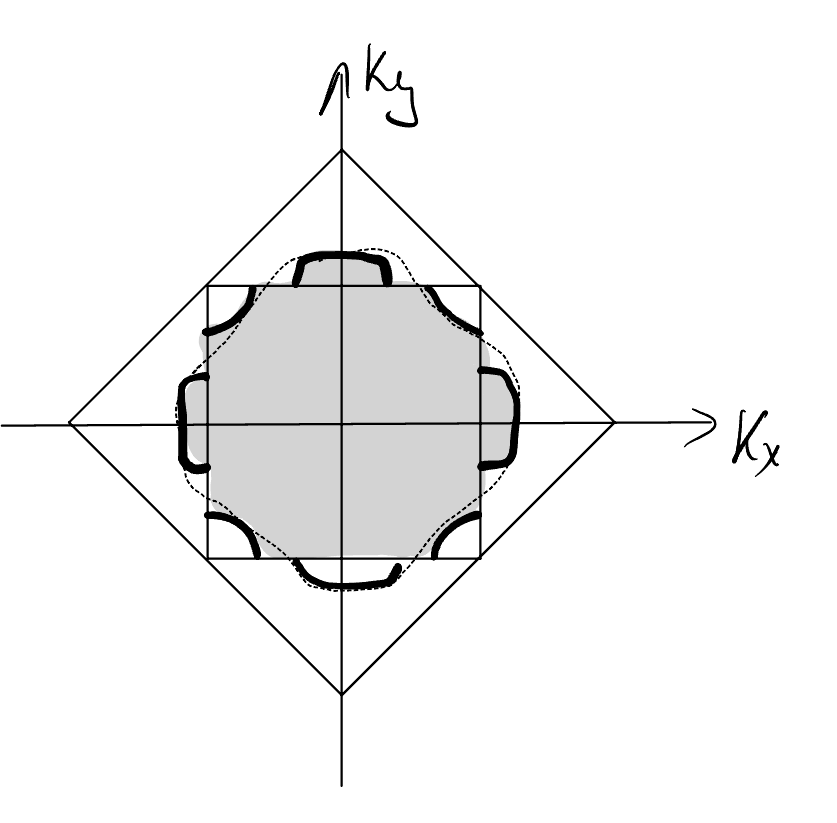
\includegraphics[width=0.2\textwidth]{phys_2_4}
\end{figure}

\textbf{Метод Харрисона построения поверхностей Ферми металлов}

\begin{figure}[h!]
    \centering
    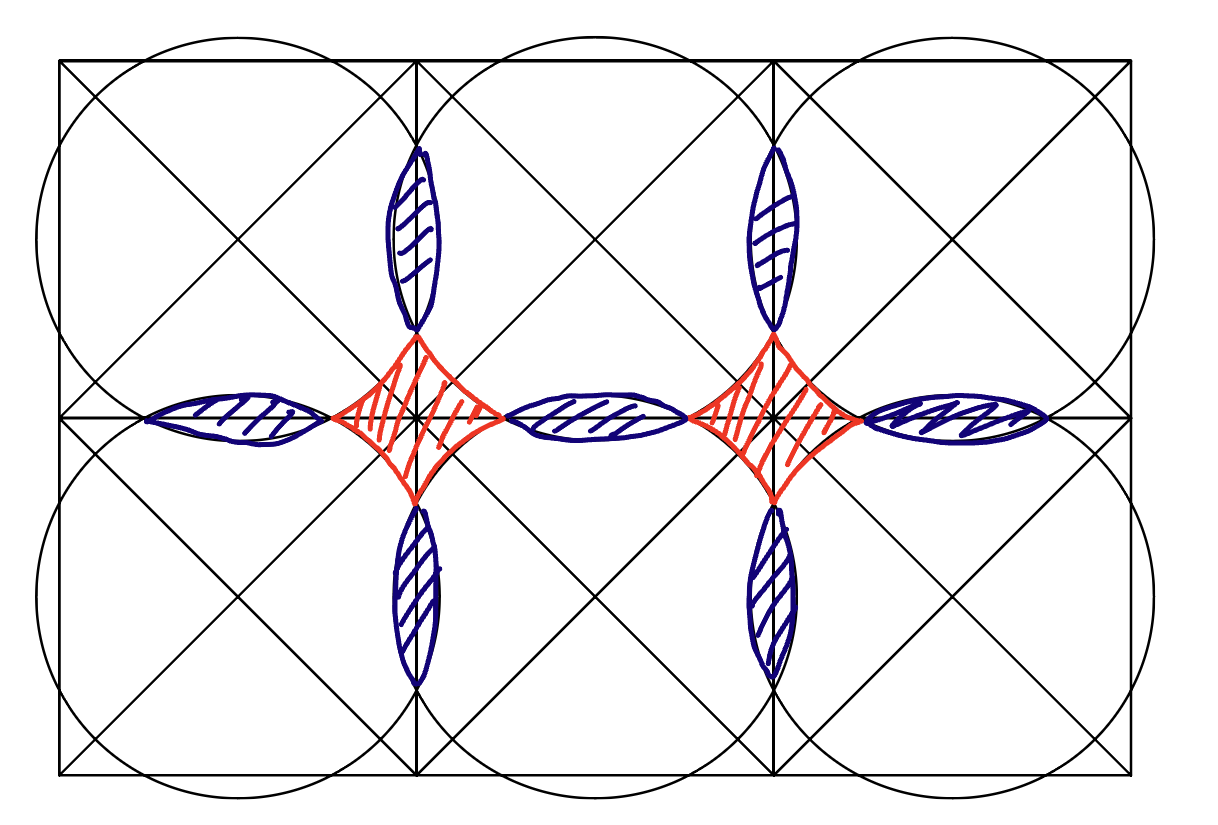
\includegraphics[width=0.4\textwidth]{phys_2_6}
\end{figure}


\begin{enumerate}
    \item Построение мозаики зон Бриллюэна
    \item Расчёт размеров и построение сфер Ферми с центрами из каждого элемента мозаики
    \item Корректировка границ сфер (пересечение с границами зон под прямым углом)
    \item Классификация полученных объёмов по зонам Бриллюэна (вогнутые поверхности --- к сферам $k+1$-й зоне (дырочные); выпуклые --- электронные в $k$-й зоне)
\end{enumerate}


\section{Предположения и следствия метода сильной связи. Заполнение энергетических зон электронами (металлы, полупроводники и диэлектрики, полуметаллы).}

\begin{figure}[h!]
    \centering
    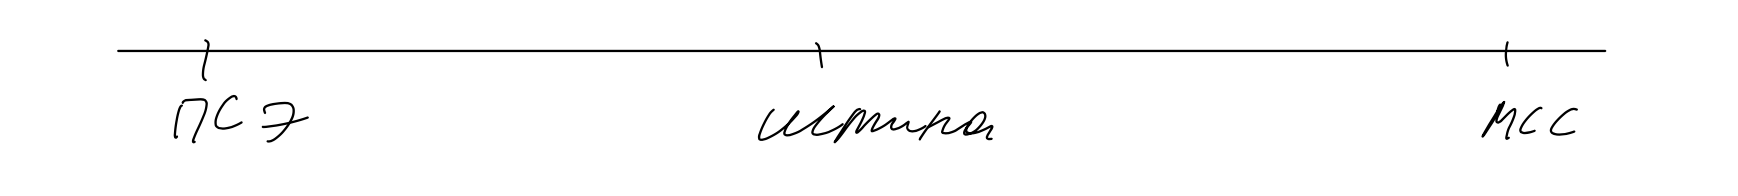
\includegraphics[width=0.8\textwidth]{phys_1_3.png}
\end{figure}

\textbf{Метод сильной связи:} электрон в твёрдом теле ведёт себя так же, как в изолированном атоме.

\begin{figure}[h!]
    \centering
    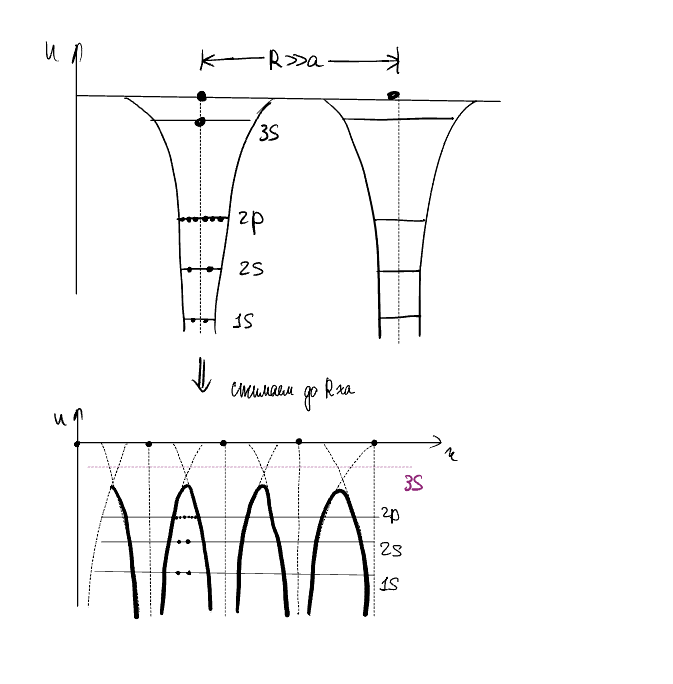
\includegraphics{phys_3_1}
\end{figure}

$\displaystyle -n=1,2,3 \ldots\left(H: E=-\frac{R_y}{n^{2}}\right)$ ($E=E(n, \;l)$ в отсутствие полей)

$\displaystyle -l=0,1,2 \ldots \mathrm{n}-1\left(M_{e}=\hbar \sqrt{l(l+1}\right)$

$\displaystyle -m=-l \ldots 0 \ldots l$ ($(2 l+1)$ значений)

$\displaystyle -s= \pm 1(1 / 2)$ (s-подуровень --- вырожден, $p-$ --- трёхкратно вырожден)

Рассмотрим на примере атома натрия.

При переходе от набора изолированных атомов к кристаллу 3s-подуровень оказывается выше барьера. Поэтому движение электронов этого подуровня по всему кристаллу не ограничено. К снижению потенциальных барьеров привело перекрытие волновых функций.

\begin{wrapfigure}{R}{0.4\textwidth}
    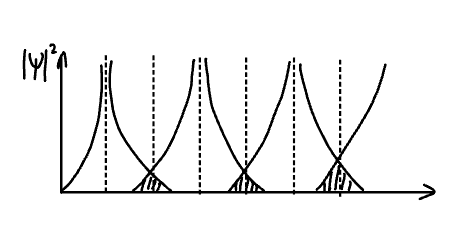
\includegraphics[width=0.4\textwidth]{phys_3_2}
\end{wrapfigure}

Уравнение Шрёдингера $\quad\left\{-\frac{\hbar^{2}}{2 m} \nabla^{2}+U(\bar{r})\right\} \psi(\bar{r})=E \psi(\bar{r}) \quad$ для изолированного атома с номером $g$ будет принимать вид $\left\{-\frac{\hbar^{2}}{2 m} \nabla^{2}+U_g(\bar{r})\right\} \psi_{g}\left(\bar{r}-\overrightarrow{R_{g}}\right)=E_{a} \psi_{g}\left(\bar{r}-\overrightarrow{R_{g}}\right)$ ($\overrightarrow{R_{g}}$ --- радиус-вектор узла решётки).

В качестве предполагаемого вида $\psi(\bar{r})$ выберем линейную комбинацию $\sum \limits_{g} a_{g} \psi_{g}$.

Тогда $\psi(\bar{r})=\sum \limits_{g} a_{g} \psi_{g}=\sum \limits_{g} e^{i k \overrightarrow{R_{g}}} \psi_{g}\left(\bar{r}-\overrightarrow{R_{g}}\right)$. При этом около узла $g$ $\psi(\bar{r}) \approx e^{i k \overrightarrow{R_{g}}} \psi_{g}\left(\bar{r}-\overrightarrow{R_{g}}\right)$

$\sum \limits_{g}\left\{\left[-\frac{\hbar^{2}}{2 m} \nabla^{2}+U_g(\bar{r})\right]+\left[U(\bar{r})-U_{g}(\bar{r})\right]-E\right\} e^{i k \overrightarrow{R_{g}}} \psi_{g}=0 \quad$ (вид, $\quad$ чтобы $\quad$ был $\quad$ известный гамельтониан $\Rightarrow \sum \limits_{g}\left\{\left(E_{a}-E\right)+W(\bar{r})\right\} e^{i k \overrightarrow{R_{g}}} \psi_{g}=0$.

$\displaystyle \int \psi_{g}^{*} \psi_{g} d \bar{r}=S\left(R_{g}-R_{g}{ }^{\prime}\right)$ --- интеграл перекрытия


$\displaystyle \int \psi_{g}^{*} w(\bar{r}) \psi_{g} d \bar{r}=A\left(R_{g}-R_{g}{ }^{\prime}\right)$ --- обменный интеграл 

Тогда $\displaystyle \sum \limits_{g} e^{i k \overrightarrow{R_{g}}}\left\{\left(E_{a}-E\right) S\left(\overrightarrow{R_{g}}-\overrightarrow{{R_{g}}^{\prime}}\right)+A\left(\overrightarrow{R_{g}}-\overrightarrow{R_{g}}\right)\right\}=0$.

И, вводя $\bar{q}=\overrightarrow{R_{g}}-\overrightarrow{R_{g}}:\left(E_{a}-E\right) \sum \limits_{g} e^{i k \bar{q}} S(\bar{q})+\sum \limits_{g} A(\bar{q}) e^{i k \bar{q}}=0$,

\noindent где $E$ периодичная по волновому вектору добавка: $E=E_{a}+\frac{\sum \limits_{g} A(\bar{q}) e^{i k \vec{q}}}{\sum \limits_{g} S(\bar{q}) e^{i k \vec{q}}}$.

В суммы входят сначала слагаемые I-го типа (ближайшие соседа, т.е. I сфера), затем вторая сфера и так далее. В числителе учитывается перекрывание волновых функций соседи, в знаменателе для простоты перекрывание не учитывается:

$
\displaystyle
\sum \limits_{g} S(\bar{q}) e^{i k \bar{q}} \int \psi_{g}^{*} \psi_{g} d \bar{r}+\cdots=1$ (остальные слагаемые не учитываются)

$
\displaystyle
\sum_{g} A(\bar{q}) e^{i k \bar{q}} \int \limits _{\bar{q}=0}^{\bar{q}=0} \psi_{g}^{*} w(\bar{r}) \psi_{g} d \bar{r} * 1+A_{1} \sum_{i k} e^{i \bar{k} \bar{q}}$  (второе слагаемое отвечает за соседей из первой координационной сферы)


\begin{figure}[h!]
    \centering
    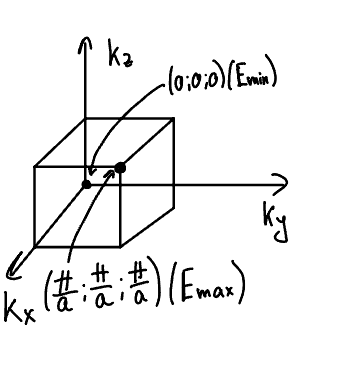
\includegraphics[width=0.2\textwidth]{phys_3_3}
\end{figure}

Конечное уравнение для $E(\bar{k}) = E_a+\underbrace{C}_{<0}+A_1 \sum e^{i\bar{k} \bar{q}}$.  В простой кубической решётке $E(\bar{k}) = E_a+C+A_1 \left( e^{i k_x a} + e^{-i k_x a} + e^{i k_y a} + e^{-i k_y a} + e^{i k_x a} + e^{-i k_z a}\right) = E_a+C+2A_1 \left( \cos k_x a + \cos k_y a + \cos k_z a\right) $

Следствия МСС:

\begin{enumerate}
    \item При образовании кристаллов из изолированных атомов каждый атомный уровень движется вниз и расширяется $\Rightarrow$ образуются зоны.
    
    \begin{figure}[h!]
        \centering
        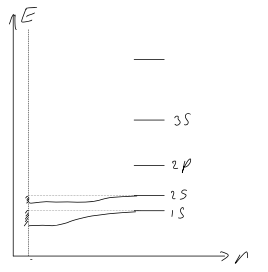
\includegraphics[width=0.4\textwidth]{phys_stripes}
    \end{figure}

    \item Каждая зона ограничена $\mathrm{E}_{\min }$ и $\mathrm{E}_{\max .}$
    
    $$
    \begin{aligned}
    & E_{\min }=E_{a}+C-6|A| \quad (\mathrm{C}<0) \\
    & E_{\max }=E_{a}+C+6|A| .
    \end{aligned}
    $$


    Таким образом, ширина зоны $12 \mathrm{~A}_{1}$ $\left(\Delta \mathrm{E}=12\left|\mathrm{~A}_{1}\right|\right)$


    \item  При движении по энергии вверх (при переходе от нижних уровней к верхним) ширина разрещённых зон растёт (внешние оболочки перекрываются сильнее, чем внутренние). При этом ширина запрещенных зон уменьшается.
    \item Разрешённые и запрещенные зоны чередуются, возможно перекрытие зон.
    \item $E(k)$ --- чётная по $k$.
    \item Качественное изменение внешних условий
    
    $\mathrm{T} \uparrow \rightarrow \mathrm{a} \uparrow \rightarrow\left|\mathrm{A}_{1}\right| \downarrow \rightarrow \Delta \mathrm{E} \downarrow \rightarrow \mathrm{E}_{\mathrm{g} \uparrow}$

    $\mathrm{P} \uparrow \rightarrow \mathrm{a} \downarrow \rightarrow\left|\mathrm{A}_{1}\right| \uparrow \rightarrow \Delta \mathrm{E} \uparrow \rightarrow \mathrm{Eg}_{\mathrm{g}} \downarrow$

    \item Вырождение может честично или полностью сниматься при образовании кристалла из атомов.
    \item Заполнение энергетических зон.
\end{enumerate}







C ростом энергии растёт ширина разрешённых зон, а ширина запрещённых зон уменьшается. Из-за высокого положения уровней в какой-то момент возможно перекрывание. При образовании кристаллов вырождение может частично или даже полностью сниматься. Отсюда качественное понимание, как меняются свойства при изменении внешних условий:

$\mathrm{T} \uparrow \rightarrow \mathrm{a} \uparrow \rightarrow\left|\mathrm{A}_{1}\right| \downarrow \rightarrow \Delta \mathrm{E} \downarrow \rightarrow \mathrm{E}_{\mathrm{g} \uparrow}$

$\mathrm{P} \uparrow \rightarrow \mathrm{a} \downarrow \rightarrow\left|\mathrm{A}_{1}\right| \uparrow \rightarrow \Delta \mathrm{E} \uparrow \rightarrow \mathrm{Eg}_{\mathrm{g}} \downarrow$

\textbf{Заполнение энергетических зон: металлы, диаэлектрики, полупроводники}

\begin{table}[h!]
    \centering
    \resizebox{\textwidth}{!}{\begin{tabular}{|c|c|}
        \hline
        N изолированных атомов & Кристалл из N атомов \\
        \hline
        $N * 2(2 l+1)$ & $2 N(2 l+1)$ (число состояний сохраняется) \\
        \hline
        \multicolumn{2}{|c|}{Число уровней сохраняется+сохраняется степень заполнения состояний}  \\
        \hline
        \end{tabular}}
\end{table}

Если в системе из N атомов уровень был заполнен наполовину, то и в кристалле зона будет заполнена наполовину.

Целиком заполненная зона не даёт вклада в проводимость.

\textbf{Классификация твёрдых тел}

\begin{figure}[h!]
    \centering
    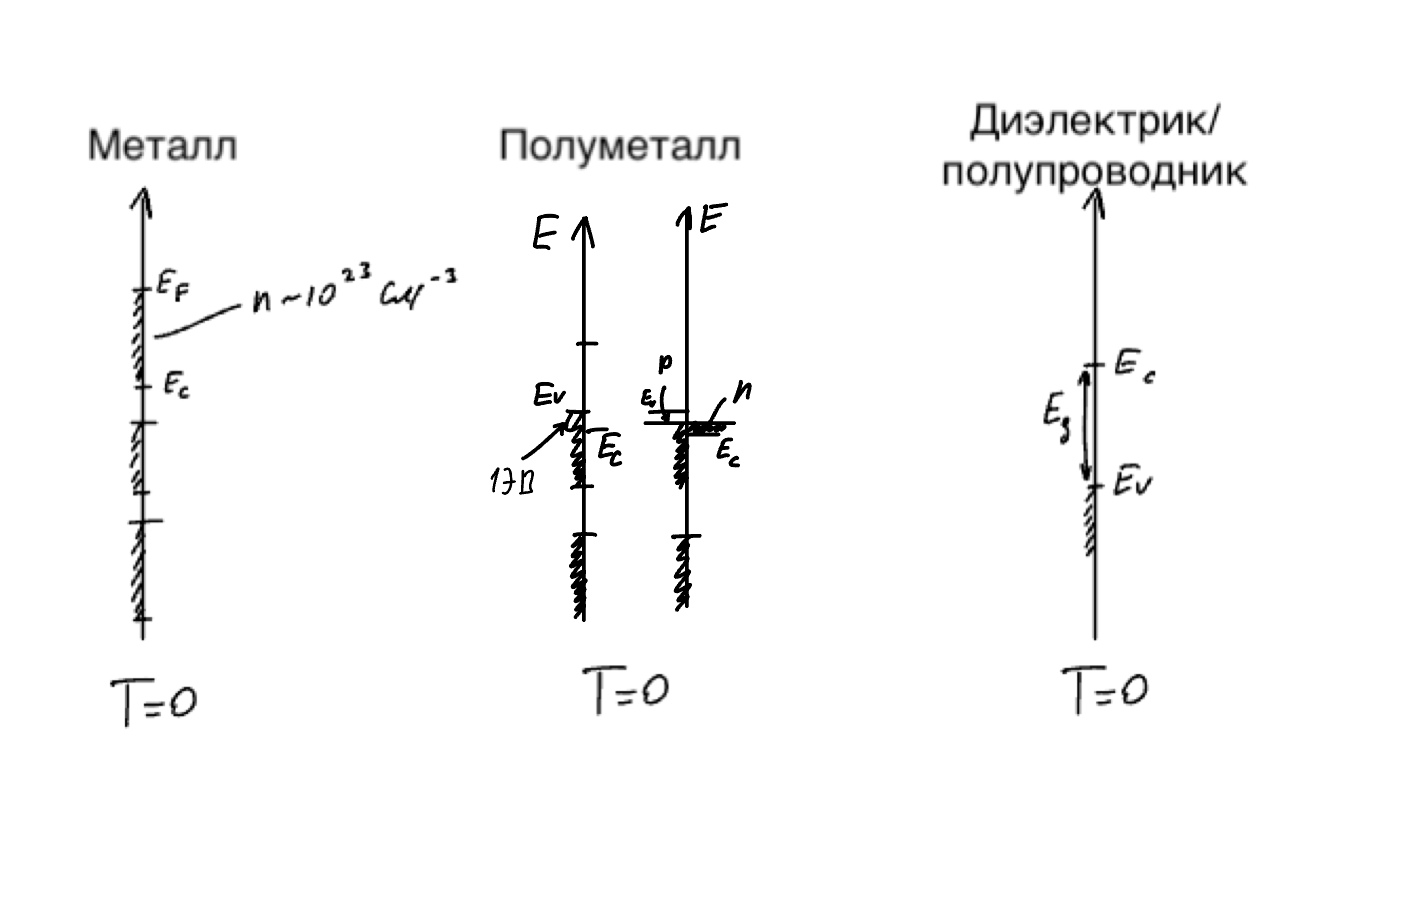
\includegraphics[width=0.8\textwidth]{images/phys_3_4.png}
\end{figure}

Полупроводник отличается от диэлектрика только размером запрещённой зоны (у диэлектрика $E_g > 5$эВ, у полупроводника $E_g < 5$эВ).


\section{Волновая функция электрона в кристалле. Теорема Блоха. Квазиимпульс электрона в кристалле. Зоны Бриллюэна.}

Для одного электрона, движущегося в кристалле, уравнение Шрёдингера имеет вид:
$$
\begin{aligned}
& \left\{-\frac{\hbar^{2}}{2 m} \nabla^{2}+U(\bar{r})\right\} \psi(\bar{r})=E \psi(\bar{r}) \\
& U\left(\bar{r}+\bar{a}_{n}\right)=U(\bar{r}), \quad \bar{a}_{n}=n_{1} \bar{a}_{1}+n_{2} \bar{a}_{2}+n_{3} \overline{a_{3}}
\end{aligned}
$$

\noindent U --- потенциал кристаллической решётки, объединяет в себе взаимодействие с решёткой и взаимодействие с другими электронами, $\bar{a_n}$ --- период кристаллической решётки. 

\textbf{Теорема Блоха:} волновая функция электрона в поле периодичного потенциала (в частности в кристалле) может быть предстравлена в виде произведения плоской волны и функции, обладающей той же периодичностью, что и кристаллическая решётка.

$$
\psi_{n k}=e^{i k r} U_{n k}(r), \quad U_{n k}(\bar{r}+\bar{a})=U_{n k}(\bar{r}) \text { --- блоховская функция }
$$

\noindent $\bar{a}$ --- период кристаллической решётки, $n$ --- номер зоны.

$\psi(\bar{r}+\bar{a})=e^{i \bar{k} \bar{a}} \psi(\bar{r})$ --- условие трансляционной симетрии для волновой функции в кристалле.

%$\psi _{\bar{k}} (\bar{r})=e ^{i \bar{k} \bar{a}} U_{\bar{k}} (\bar{r})$ --- будем искать решения уравнения Шрёдингера в виде $\widehat{H} \psi=\varepsilon \psi$

% $
% \begin{aligned}
% & U_{\bar{k}}(\bar{r})=U_{\hat{k}}(\bar{r}+\bar{a}) \text {--- периодичность функции} \\
% & \widehat{H} \psi_{\bar{k}}(\bar{r})=\hat{H} e^{i \bar{k} \bar{r}} U_{k}(\bar{r})=\hat{H} \varepsilon e^{i \bar{k} \bar{r}} U_{k}(\bar{r}) %\\
% & e^{-i \bar{k} \bar{r}} \widehat{H} e^{i \bar{k} \bar{r}} U_{\bar{k}}(\bar{r})=e^{-i \bar{k} \bar{r}} \hat{H} \varepsilon e^{i \bar{k} \bar{r}} U_{k}(\bar{r}) \\
% & \widehat{H}_{k}\left(U_{\bar{k}}(\bar{r})\right)=\varepsilon(\bar{k}) U_{\bar{k}}(\bar{r})\text { (1) (новая задача) }
% \end{aligned}
% $

% Представление волновой функции : 
% $$\psi _{n\bar{k}} = e ^{i\bar{k}\bar{r}} U_{n \bar{k}} (\bar{r}) $$


\textbf{Квазиимпульс в кристалле}


    
% $\hat{\bar{v}}=\frac{\hat{\bar{p}}}{m}=-i \frac{\hbar}{m} \nabla$

Скорость свободного электрона $ \displaystyle \langle\bar{V}\rangle=\int \limits_V A e^{-i \bar{k} \bar{r}}\left(-i \frac{\hbar}{m} \nabla\right) A e^{i \bar{k} \bar{r}} d r =  \frac{-i\hbar}{m}(i k) \underbrace{\int\limits _V A e^{-i \bar{k} \bar{r}} A e^{i \bar{k} \bar{r}} d r}_1 =\frac{\hbar k}{m}=\frac{p}{m}$

p--- импульс.


Скорость электрона в кристалле $\langle \bar{V} \rangle=\int \limits_V \psi^*(\bar{r}) \hat{\bar{V}} \psi(\bar{r}) d \bar{r}$

$\displaystyle \langle\bar{V}\rangle=\int u_k^*(\bar{r}) e^{-i \bar{k} \bar{r}}\left(-i \frac{\hbar}{m} \nabla\right) U_k(\bar{r}) e^{i \bar{k} \bar{r}} d r=  -\left(i \frac{\hbar}{m}\right)(i k) \int u_k^*(r) e^{-i k r} u_k(r) e^{i k r} d r+  \left(-i \frac{\hbar}{m}\right) \int u_k^*(r) e^{-i k r} e^{i k r} \nabla u_k(r) d r= \frac{\hbar k}{m}-i \frac{\hbar}{m} \int u_k^*(r) \nabla u_k(r) d r \neq \frac{p}{m}$

\bigskip

Для описания поведения электрона в кристалле вводится квазиимпульс $P$ такой, что $\displaystyle V=\frac{dE}{dP}$. Вместе с квазиимпульсом вводится квазиволновой вектор $k=P/\hbar$. Далее кразиимпульс будем обозначать $p$.

\textbf{Свойства квазиимульса:}
\begin{enumerate}
    \item $\displaystyle \frac{dp}{dt}=F=\nabla U$, причём $F$ --- внешняя сила.
    \item При отсутствии внешних сил квазиимпульс сохраняется.
    \item Любое искажение периодичности решётки, приводящее к процессам рассеяния электронов на дефектах, можно представить как наложение локальной внешней силы.
    \item Квазиимпульс дискретен ($\Delta p = 2\pi \hbar /a$).
    \item Квазиимпульс изменяется в пределах зоны Бриллюэна (в то время как импульс свободного электрона может принимать значения $[0; +\infty)$)
\end{enumerate}

Возьмём большой кристалл ($L \gg a$). Внутреннюю область разбиваем на блоки размером $L_x$, $L_y$, $L_z$.
$\psi(x; y; z) = \psi(x +L_x; y; z) = \psi(x; y+L_y; z) = \psi(x; y; z+L_z)$

$\psi(x+L_x)=\psi(x) \Rightarrow U_{k}(x+L_x)e^{ik_{x} (x+L_x)}=U_k(x)e^{ik_{x} x}$

Так как $e^{ik_{x} L_x}=1$, то $k_x L_x=2 \pi n$ ($n$ --- целое). Из этого следует дискретность квазиволнового вектора, так как $p=\hbar k$, то и дискретность квазиимпульса.

\textbf{Зона Бриллюэна} --- отображение ячейки Вигнера-Зейтса в обратном пространстве. В приближении Блоха волновая функция электрона для периодического потенциала решетки полность описывается ее поведением в 1 зоне Бриллюэна. 1я зона Бриллюэна содержит точку $k=0$ (2я зона непосредственно прилегает к 1 и так далее); она может быть построена как объем, ограниченный плоскостями, которые отстоят на равные расстояния от рассматриваемого узла обратной решетки до соседних узлов. Для простой кубической решетки зона Бриллюэна --- кубооктаэдр (14-граник).

\begin{figure}[h!]
    \centering
    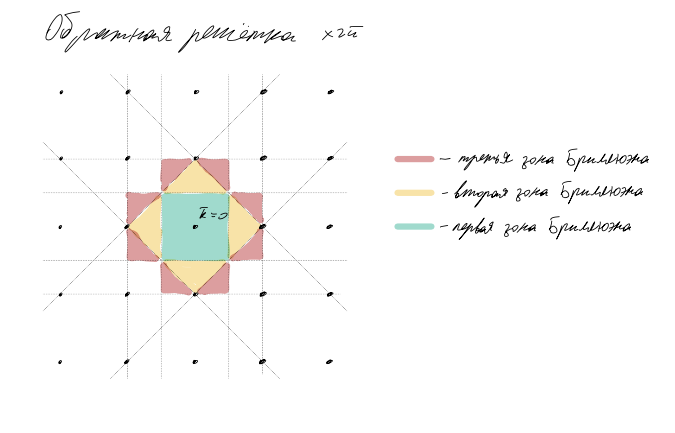
\includegraphics[width=0.8\textwidth]{phys_4_1.png}
\end{figure}

Число разрешённых (возможных) состояний квазиволнового вектора в зон Бриллюэна конечно. Число разрешённых состояний в кристалле с параметром решётки $a$ и периодичностью квазиволнового вектора $2\pi /L$: $\frac{2\pi}{a} / \frac{2\pi}{L} = 2 L/a = 2N$. $N$ --- количество атомов в атомной решётке, 2 из-за возможных ориентаций спина.

Все зоны Бриллюэна имеют одинаковый объём.



\section{Закон дисперсии, изоэнергетическая поверхность, эффективная масса электрона в кристалле}

\textbf{Закон дисперсии} --- зависимость энергии от квазиимпульса в разрешенной зоне ($E(p)$).

\textit{Классификация:}

\begin{enumerate}
    \item Квадратичные ($E \sim p^2$)
    \begin{enumerate}
        \item Квадратичный изотропный $E=\frac{p^2}{2 m^*}$ (изоэнергетическая поверхность --- сфера, $R=\sqrt{2m^*E}$)
        \item Квадратичный анизотропный $E=\frac{p_x^2}{2 m_x}+\frac{p_y^2}{2 m_y}+\frac{p_z^2}{2 m_z}$ (изоэнергетическая поверхность --- трёхосный эллипсоид. Для случая $m_x=m_y$ --- эллипсоид вращения).
    \end{enumerate}
    \item Неквадратичные ($E \nsim p^2$, $m^* \neq const \quad m^* \uparrow \uparrow E$)
    \begin{enumerate}
        \item Закон Кейна (изотропный) $E(1+\frac{E}{E_g})=\frac{p^2}{2m^*}$ (изоэнергетическая поверхность в близи экстремума --- сфера $R=\sqrt{2m^*(0)E(1+E/E_g)}$)
        \item Закон дисперсии в методе сильной связи (для ПКР) $E=E_a+C+2 A_1\left(\cos \left(k_x a\right)+\cos \left(k_y a\right)+\cos \left(k_z a\right)\right)$ (В окрестностях экстремумов выраждается в квадратичный закон $E=|A_1|a^2k^2$, изоэнергетическая поверхность в близи экстремума --- сфера $R=\sqrt{E/(|A_1|a^2)}$)
    \end{enumerate}
\end{enumerate}

\textbf{Эффективная масса электрона}

Введение эффективной массы электрона позволяет описывать его движение в кристалле при помощи законов механики. $\displaystyle \frac{1}{m^*} = \frac{d^2E}{dp^2}$. В близи минимума энергии $m^*>0$, в близи максимума энергии $m^*<0$. 

В трёхмерном случае $m^*$ --- тензор, который можно диагонализировать правильным выбором точки отсчёта.


$$
    \widetilde{m^*}^{-1}=\left(\begin{array}{ccc}
    \frac{\partial^2 E}{\partial p_x^2} & \frac{\partial^2 E}{\partial p_x \partial p_y} & \frac{\partial^2 E}{\partial p_x \partial p_z} \\
    \frac{\partial^2 E}{\partial p_y \partial p_x} & \frac{\partial^2 E}{\partial p_y^2} & \frac{\partial^2 E}{\partial p_y \partial p_z} \\
    \frac{\partial^2 E}{\partial p_z \partial p_x} & \frac{\partial^2 E}{\partial p_z \partial p_y} & \frac{\partial^2 E}{\partial p_z^2}
    \end{array}\right) \rightarrow \left(\begin{array}{ccc} m_1^{-1} & 0 & 0 \\ 0 & m_2^{-1} & 0 \\ 0 & 0 & m_3^{-1} \end{array}\right)
$$

$\bar{F}_\text{внеш} =  \widetilde{m^*}\bar{a}$

\section{$\rm k \cdot p$--метод. Энергетический спектр электрона в однозонном приближении. Правила сумм. Взаимодействие энергетических зон}

\textbf{$\rm k \cdot p$--метод.}

Методы расчёта <<из первых принципов>> не обладают достаточной точностью для расчёта энергетических зон узкощелевых полупроводников так как:

\begin{enumerate}
    \item $E_g$ в данных материалах может быть <0,1эВ (или 0эВ)
    \item Результат получается в численном виде (таблица с числами в пределах зоны Бриллюэна). В УЩПП необходимо знать закон дисперсии в окрестности экстремумов зон ($E_c (k)$ и $E_v (k)$) в аналитическом виде.
\end{enumerate}

Преимущество $\rm k \cdot p$--метода --- при расчёте используются экспериментальные данные, а в результате получается аналитический вид закона дисперсии.

\textbf{Предположения:}

\begin{itemize}
    \item $\psi _{n k_0}(\bar{r})$ --- волновые функции в экстремумах зон
    \item $E_n(\bar{k_0})$ --- энергия краёв зон
    \item Матричные элементы оператора импульса (из эксперимента)
\end{itemize}
 То есть известны решения уравнения Шрёдингера $\displaystyle \left\{\frac{\widehat{\bar{p}^2}}{2 m}+U(\bar{r})\right\} \psi_{n k_0}(\bar{r})=E_n\left(\bar{k}_0\right) \psi_{n k_0}(\bar{r})$. Можно найти $\displaystyle \left\{\frac{\widehat{\bar{p}^2}}{2 m}+U(\bar{r})\right\} \psi_{n k_0}(\bar{r})=E_n\left(\bar{k}_0\right) \psi_{n k}(\bar{r})$ в малых окрестностях экстремумов зон $k_0$. То есть можно найти законы дисперсии.

 \begin{figure}[h!]
    \centering
    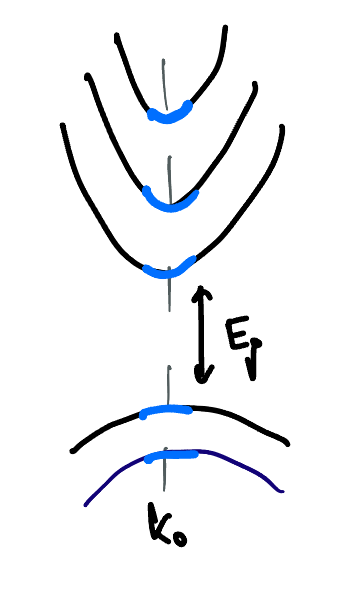
\includegraphics[width=0.2\textwidth]{phys_7_1}
    
 \end{figure}

 \begin{enumerate}
    \item Переход от уравнения для $\psi_{nk}$ к уравнению $U_{nk}$. 
    
    $\psi_{n k}(\bar{r})=U_{n k}(\bar{r}) e^{i \bar{k} \bar{r}}$ 
    
    $\displaystyle \psi_{n k}(\bar{r})=U_{n k}(r) e^{i \bar{k} \bar{r}} \hat{\bar{p}}\left(U_{n k} e^{i \bar{k} \bar{r}}\right)=e^{i \bar{k} \bar{r}} \hat{\bar{p}} \left( U_{n k} \right) + U_{n k} \hat{\bar{p}} \left( e^{i \bar{k} \bar{r}} \right) =e^{i \bar{k} \bar{r}} \hat{\bar{p}} \left( U_{n k} \right)+ \hbar k  e^{i \bar{k} \bar{r}}U_{n k}= e^{i \bar{k} \bar{r}}(\hat{\bar{p}}+\hbar \bar{k}) U_{n k}$
    
    $\hat{\bar{p}} \left( \hat{\bar{p}}\left(u_{n k} e^{i \bar{k} \bar{r}}\right) \right) =\ldots=e^{i \bar{k} \bar{r}}(\hat{\bar{p}}+ \hbar \bar{k})^2 U_{n k}$
    
    $\displaystyle \underbrace{\left\{\frac{(\hat{\bar{p}}+\hbar k)^2}{2 m}+U(\bar{r})\right\}}_{\hat{H}_k} U_{nk}(\bar{r}) =E_n(\bar{k}) U_{n k}(\bar{r})$


    $\hat{\bar{p}} \overset{\psi_{nk} \rightarrow U_{nk}}{\longrightarrow} (\hat{p}+\hbar k)$

    $\left\{\frac{(\hat{\hat{p}}+\hbar k)^2}{2 m}+U(\bar{r})\right\}=\hat{\mu}_k$

    \item Выделение оператора $\hat{H}_{k_0}$ и дополнительного возмущения зависящего от $(k-k_0)$
    
    $\displaystyle \hat{H}_k=\frac{\hat{\bar{p}}^2}{2 m}+\frac{\hbar}{m} \bar{k}\bar{p}+\frac{\hbar^2 k^2}{2 m} +U(\bar{r})$
    
    $\displaystyle \hat{H}_k=\hat{H}_{k_0}+\hat{V}$
    
    $\displaystyle \hat{H}_k=\hat{H}_{k_0}+\frac{\hbar}{m}\left(\bar{k}-\hat{k}_0\right) \hat{\bar{p}}+\frac{\hbar^2}{2 m}\left(\bar{k}-\bar{k}_0\right)$
    
    $\displaystyle \hat{V}=\frac{\hbar}{m}\left(\bar{k}-\bar{k}_0\right) \hat{\bar{p}}+\frac{\hbar^2}{2}\left(\bar{k}-\bar{k}_0\right) $

    $\hat{V}$ --- возмущение.

    $\displaystyle \hat{V}$ возрастает при удалении $\bar{k}$  от $\bar{k}_0$.

    \item Применяем теорию возмущений. Разложение $U_{nk}(\bar{r})$ в ряд по известным $U_{nk_0}(\bar{r})$. Подставляем в уравнение, умножаем на $U^*_{nk_0}$, интегрируем по элементарной ячейке. Переходим к системе уравнений относительно $C_{nn^\prime}$
    
    $\sum_{n^{\prime}} C_{n n^{\prime}}\left[\int U_{n k_0}^* \hat{H}_{k_0} U_{n^{\prime} k_0} d \bar{r}\right. +\frac{\hbar}{m}\left(\bar{k}-\bar{k}_0\right) \int U_{n k_0}^* \hat{\bar{p}} U_{n^{\prime} k_0} d \bar{r}^*\left.+\frac{\hbar^2}{2 m}\left(\bar{k^2}- \bar{k^2}_0\right) \int U_{n k_0}^* U_{n^{\prime} k_0} d r\right]= \sum_{n^{\prime}} C_{n n^{\prime}} E_n(\bar{k}) \underbrace{\int U_{n k_0}^* U_{n^{\prime} k_0} d r}_{\delta_{n n_1}}$

    $\int U_{n k_0}^* \hat{H}_{k_0} U_{n^{\prime} k_0} d \bar{r} = E_n (\bar{k}_0)\delta_{nn^\prime}$
    
    $\left\langle U_{n k_0}|\hat{\bar{p}}| U_{n^{\prime} k_0}\right\rangle=p_{n n^{\prime}}\left(\bar{k}_0\right)$ --- матричный оператор импульса.

    \item Определитель системы должен быть равен <<0>>
    
    $\mathrm{det} \Bigg| \left[\left\{E_1(\bar{k}_0)-E_n(\bar{k})+\frac{\hbar^2}{2 m} \right\} \delta_{n n^{\prime}}+\frac{\hbar}{m}(\bar{k}-\bar{k}_0) p_{n n^{\prime}}(\bar{k}_0)\right]  \Bigg| =0$

    В общем случае $n=\infty$

 \end{enumerate}

Решая определитель можно получить законы дисперсии для $E_n(\bar{k})$. Мешает то, что надо знать много значений оператора импульса и наличие большого количества зон.

\textbf{Однозонное приближение}

1 зона с номером $n$. В идём в конец 3 пункта, $n=n^\prime$. $E(\bar{k}_0) - E(\bar{k}) + \frac{\hbar}{2m}(\bar{k}^2 - \bar{k}^{2}_0) + \frac{\hbar}{m}(\bar{k} - \bar{k}_0)\bar{p}_{nn}(\bar{k}_0)=0$

Воспользовавшись $p_{A n}(k_0)=-\hbar k_0$ получаем $E(\bar{k})=E\left(\bar{k}_0\right)+\frac{\hbar^2\left(\bar{k}-\bar{k}_0\right)^2}{2 m}$.

\textbf{Правила сумм}

Вернёмся в конец пункта 2.

$\mathrm{H}=\hat{H}_{k_0}+\frac{\hbar}{m}\left(\bar{k}-\bar{k}_0\right) \hat{\bar{p}}+\frac{\hbar^2}{2 m}\left(\bar{k}^2-\bar{k}_0^2\right)$

В теории возмущений для невырожденных состояний 

$\left(\hat{H_0}+\hat{U}\right) \psi=E \psi \quad E=E_0+E_1+E_2+\ldots$

$E_1=V_{n n}=\int \psi_n^* \hat{V} \psi_n d r$

$E_L=\sum_{n^{\prime} \neq n} \frac{V_{n n^{\prime}} \cdot V_{n^{\prime} n}}{E_n(0)-E_{n^{\prime}}(0)}$

$E_n(\bar{k})=E_n\left(\bar{k}_0\right)+\underbrace{\frac{\hbar}{m}\left(\bar{k}-\bar{k}_0\right) \int U_n^* \hat{М} U_n d r+\frac{\hbar^2}{2 m}\left(k^*-k_0^2\right) \int U^* U d r}_{E_1} + \underbrace{\frac{\hbar^2}{m^2} \sum_{n^{\prime} \neq n} \frac{\left(k-k_0\right) p_{n n^{\prime}}\left(\bar{k}_0\right) \cdot\left(k-k_0\right) p_{n^{\prime} n}\left(\bar{k}_0\right)}{\left(E_n \bar{k}_0\right)-E_{n^{\prime}}\left(\bar{k}_0\right)}}_{E_2} + E_3+ \ldots$

$\hbar (\bar{k}-\bar{k}_0)=\bar{p}$ --- квазиимпульс.

$E=E_n\left(E_0\right)+\frac{p^2}{2 m^*}$

$\displaystyle 
\left.\begin{array}{l}\frac{1}{m^*}=\frac{1}{m}+\frac{2}{m^2} \sum \frac{p_{n n}\left(\bar{k}_0\right) p_{n^\prime n}\left(k_0\right)}{E_n\left(k_0\right)-E_{n^{\prime}}\left(k_0\right)}+\ldots \\ E_n(\bar{k})=E_n\left(\bar{k}_0\right)+\frac{p^2}{2 m}+\frac{1}{m^2} \sum_{n^\prime \neq n} \frac{\bar{p} \bar{p}_{n^\prime n}\left(k_0\right) \cdot \bar{p} \bar{p}_{n^\prime n }\left(k_0\right)}{E_n\left(k_0\right)-E_{n^\prime}\left(k_0\right)}+\ldots\end{array}\right\} \text{--- правила сумм}$

\textit{Правила сумм} для $E_n(\bar{k})$ и $m^*$:

\begin{enumerate}
    \item Отклонение сумм для $E_n(\bar{k})$ от квадратичного изотропного закона и $m^*$ от $m$ --- следствие учёта наличия других зон.
    \item Вклад других зон --- знакопеременный.
    \item Количественно ряд зависит от $E_n-E_{n^\prime}$ и от величины $p_{nn^\prime}(\bar{k}_0)$.
\end{enumerate}

Если $p_{nn^\prime}(\bar{k}_0)=0$, то зоны не взаимодействуют. Если $p_{nn^\prime}(\bar{k}_0)\neq 0$, то говорят, что зоны взаимодествуют.


\section{Параметры зонной структуры полупроводников. Зонная структура основных полупроводниковых материалов.}

\textbf{Основные параметры зонной структуры:}

\begin{enumerate}
    \item Кристаллическая решётка
    \item Форма зоны Бриллюэна и расположение в ней основных точек симметрии и направлений
    \item Положение экстремумов зон в зоне Бриллюэна, величина $E_g$.
    \item Законы дисперсии и изоэнергетические поверхности в окрестностях экстремумов зон.
\end{enumerate}

\textit{//для справки//}

Для ГЦК решётки 1 зона Бриллюэна --- кубооктаэдр в ней

$\Gamma$ --- центр зоны Бриллюэна

$X$ --- центры квадратных граней (3 штуки)

$L$ --- центры гексогональных граней (4 штуки)

$\Sigma$ --- внутри зоны Бриллюэна в направлении типа $\langle 110 \rangle$ (12 штук)

$\Delta$ --- внутри зоны Бриллюэна в направлении типа $\langle 100 \rangle$ (6 штук)



\textbf{Зонная структура Ge и Si}

\begin{enumerate}
    \item Кристаллическая решётка типа алмаза (2 ГЦК подрешётки, сдвинутые друг относительно друга на $\frac{1}{4}$ пространственной диагонали куба)
    \item Зона Бриллюэна такая же как и у ГЦК решётки Браве --- 14-гранник
    \item Ge: минимум зоны проводимости в точках $L$ (4 точки на зону Бриллюэна). максимум валентной зоны в точке $\Gamma$ (1 точка)
    
    $E_g \approx 0,67$~эВ при $T=300$~К

    Si: минимум зоны проводимости в точках $\Delta$ (6 штук на зону Бриллюэна), максимум валентной зоны в точке $\Gamma$ (1 точка)
    
    $E_g \approx 1,1$~эВ при $T=300$~К

    \begin{figure}[h!]
        \centering
        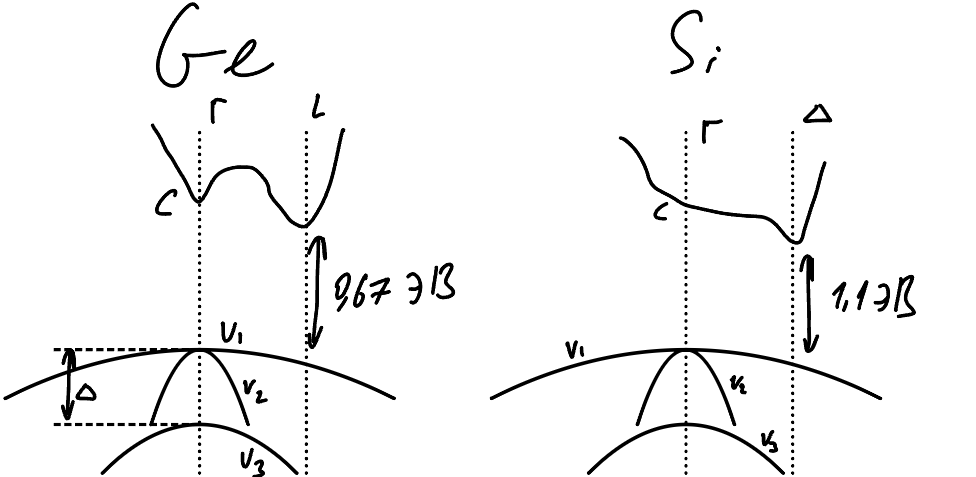
\includegraphics[width=0.5\textwidth]{phys_8_1}
    \end{figure}

    \item Зона проводимости: $\displaystyle E(\bar{k}) = \frac{\hbar^2 k_\perp ^2}{2m_t^*} + \frac{\hbar^2 k_\parallel ^2}{2m_l^*}$
    
    $k_\perp ^2 = k_x ^2 + k_y ^2$, $k^2_\parallel = k^2 _z$

    Ge: $k_\parallel \parallel \langle 111 \rangle$

    Si: $k_\parallel \parallel \langle 100 \rangle$

    Изоэнергетические поверхности --- эллипсоиды вращения.

    \item Валентная зона: $\displaystyle E_{1;2}=-\frac{\hbar^2}{2m}\left[ Ak^2 \pm \left( B^2k^4 + c^2(k_x^2k_y^2+ k_y^2k_z^2 + k_x^2k_x^2) \right)^0,5 \right]$, (A, B, C --- безразмерные константы). Изоэнергетические поверхности --- гофрированные сферы.
    
    $E_3 (\bar{k})=-\frac{\hbar^2 \bar{k}^2}{2m^*_3}$, $m^*_3=\frac{m}{A}$. Изоэнергетические поверхности --- сферы.
\end{enumerate}





\textbf{Зонная структура $A^3B^5$}

A: In, Ga, Al...

B: Sb, As, P, N...

Общая (наиболее распространённа)я ситуация

\begin{enumerate}
    \item Кристаллическая решётка типа сфалерита (цинковой обманки)
    \item Зона Бриллюэна --- кубооктаэдр
    \item Закон дисперсии Кейна
\end{enumerate}

\begin{figure}[h!]
    \centering
    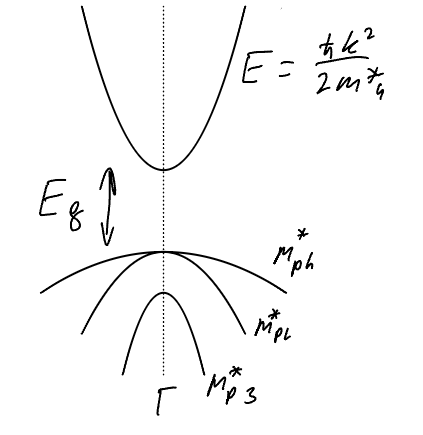
\includegraphics[width=0.4\textwidth]{phys_8_2}
\end{figure}

Отклонение от этой системы:

\begin{itemize}
    \item GaN, InN, AlN кристаллизуются в решётки вюрцита (ГПУ)
    \item Наличие у ряда полупроводников дополнительных экстремумов в зоне проводимости
\end{itemize}

\begin{figure}[h!]
    \centering
    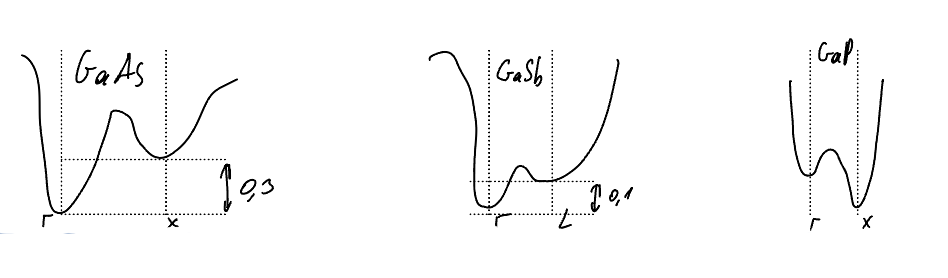
\includegraphics[width=0.8\textwidth]{phys_8_3}
\end{figure}

\begin{figure}[h!]
    \centering
    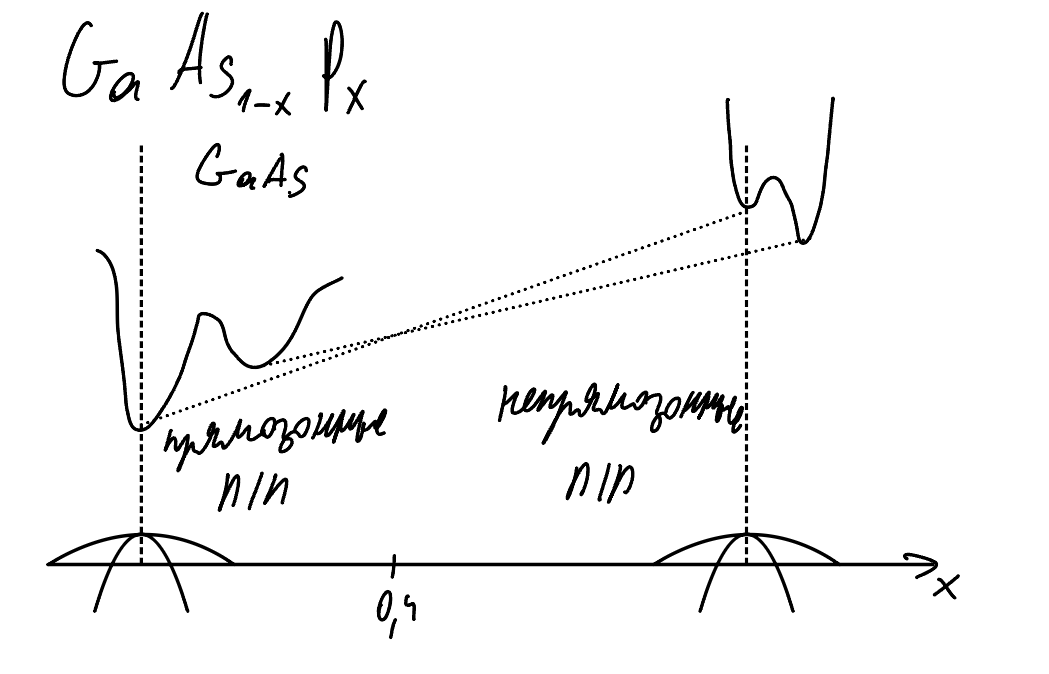
\includegraphics[width=0.7\textwidth]{phys_8_4}
\end{figure}

Прямозонные используются в оптике.


\textbf{Зонная структура $A^2B^6$}

A: Zn, Cd, Hg...

B: O, Se, S, Te...

\begin{enumerate}
    \item Кристаллическая решётка типа сфалерита или вюрцита
    \item Зона Бриллюэна --- кубооктаэдр
    \item Выполняется закон Кейна
\end{enumerate}

Особенности полупроводников на основе Hg:

\begin{enumerate}
    \item При низких температурах существуют свободные носители заряда (как в металлах)
    \item Инверсная зонная структура ($E_g<0$ в законе Кейна)
\end{enumerate}

\begin{figure}[h!]
    \centering
    \subfigure{
    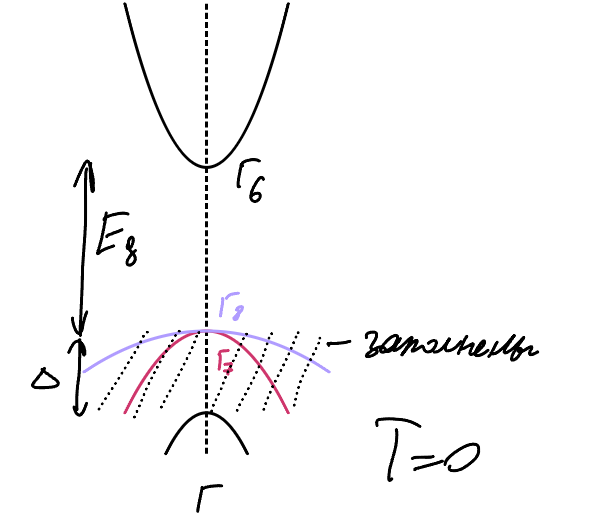
\includegraphics[width=0.4\textwidth]{phys_8_5}}
    \subfigure{
    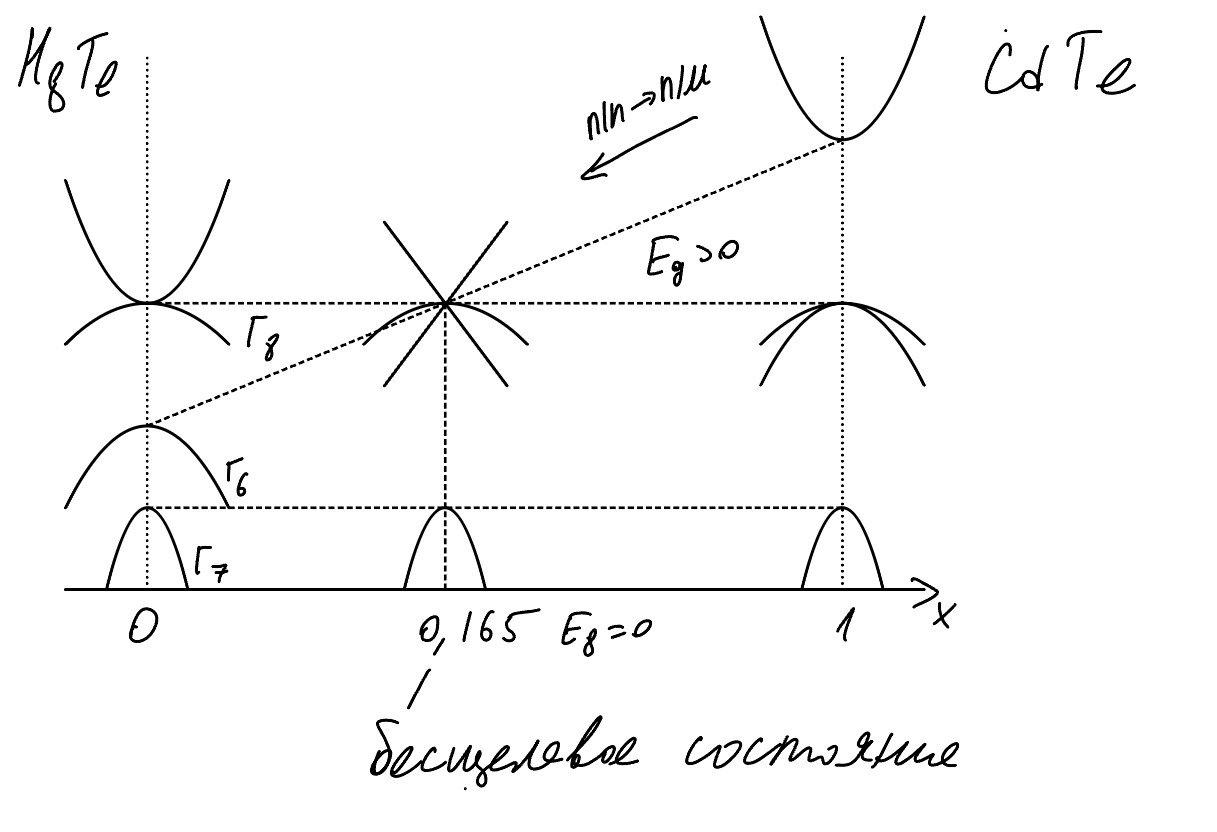
\includegraphics[width=0.5\textwidth]{phys_8_6}}
\end{figure}


\textbf{Зонная структура $A^4B^6$}

A: Sn, Ge, Pb...

B: O, S, Se, Te...

\textit{Кристаллическая структура}

\begin{enumerate}
    \item Кубические модификации (решётки типа NaCl). Зона Бриллюэна --- кубооктаэдр
    \item Ромбическая решётка (деформация куба вдоль $\langle 111 \rangle$) (CdTe)
    \item Орторомбическая (деформация куба вдоль $\langle 110 \rangle$) (PbTe)
\end{enumerate}


\vspace{2cm}

\begin{figure}[h!]
    \centering
    %
    \subfigure{
        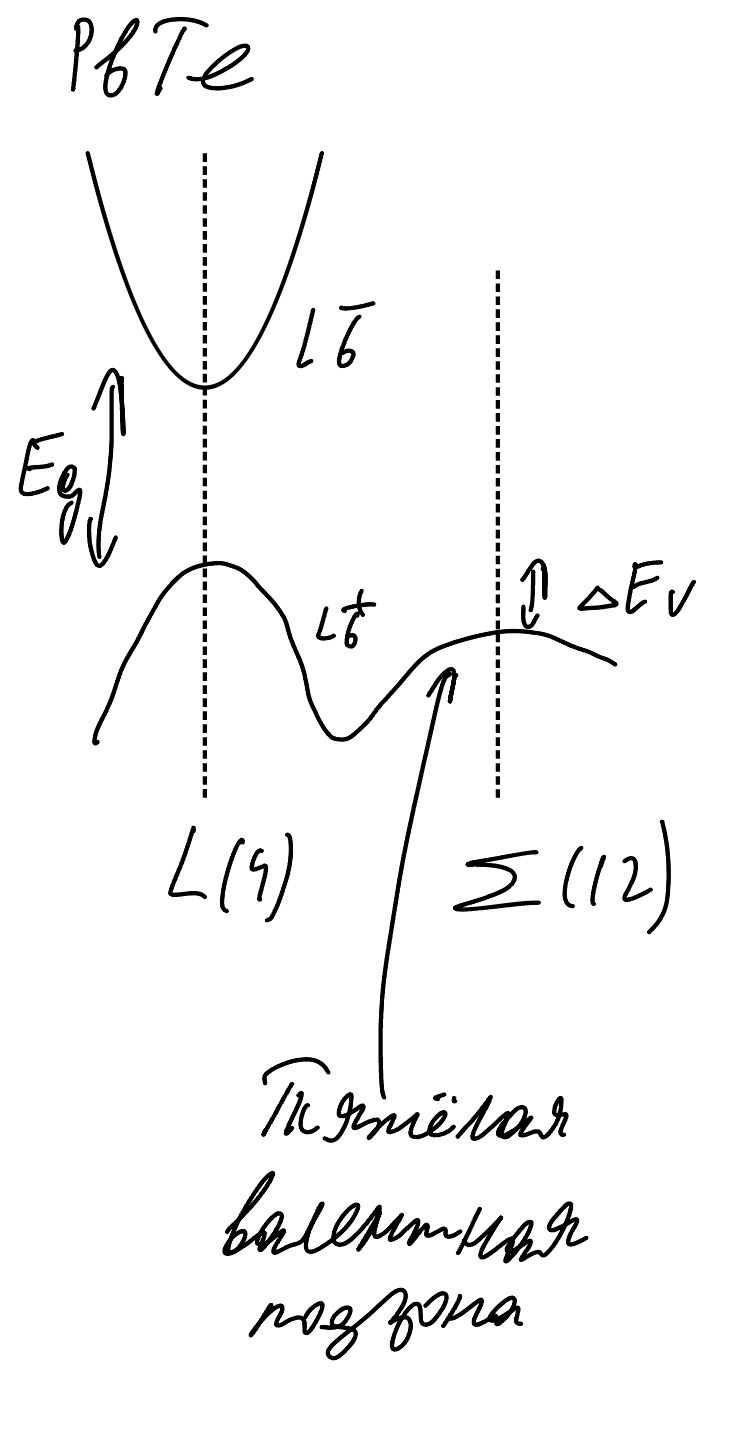
\includegraphics[width=0.2\textwidth]{phys_8_7}}
    \subfigure{
    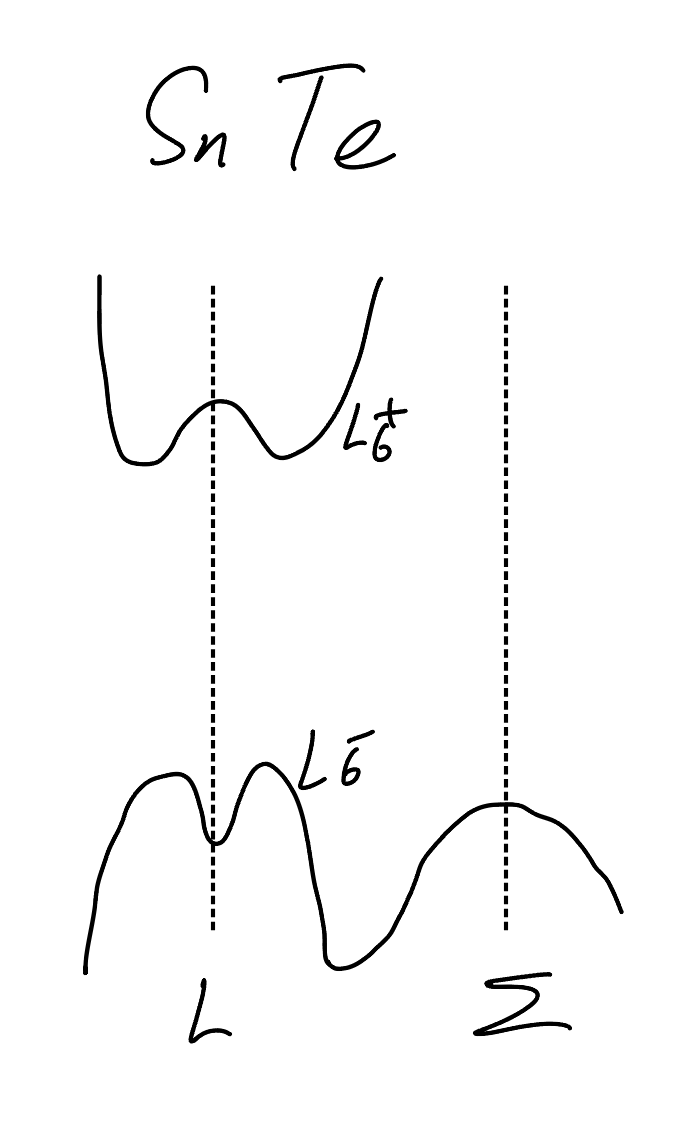
\includegraphics[width=0.2\textwidth]{phys_8_8}}
\end{figure}



\vfill

\textbf{Модель инверсии зон Диммака}

\begin{figure}[h!]
    \centering
    \subfigure{
    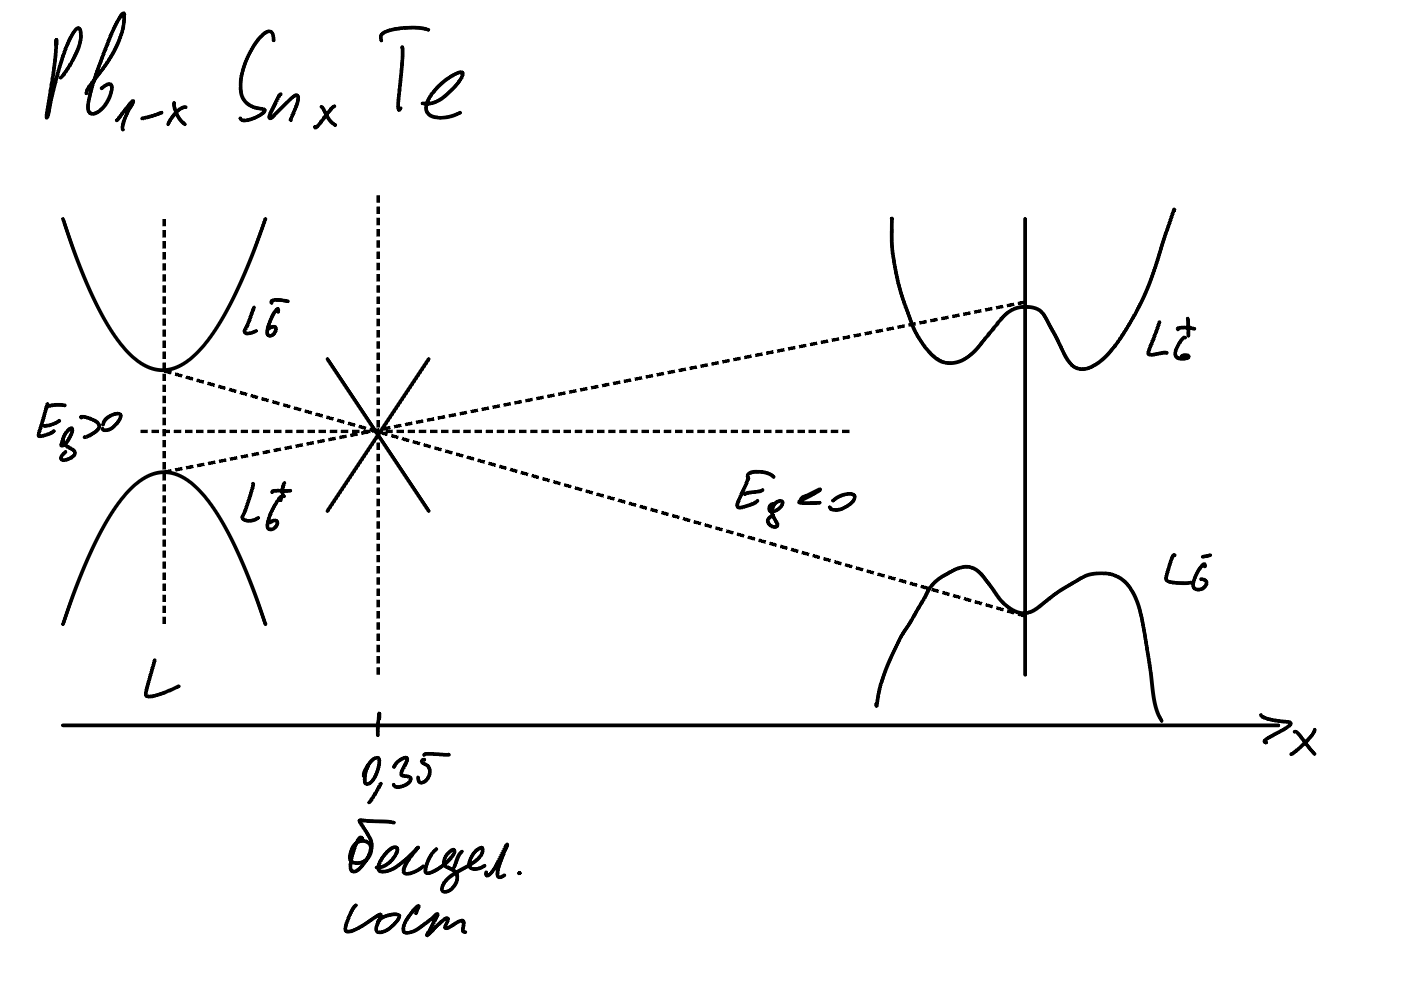
\includegraphics[width=0.45\textwidth]{phys_8_9}}
    \subfigure{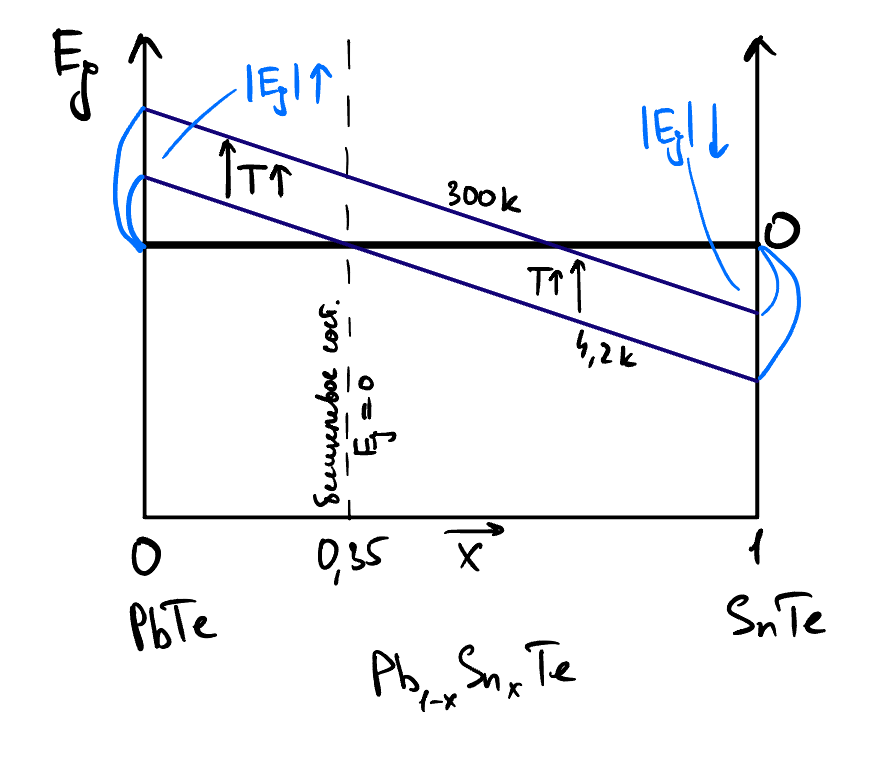
\includegraphics[width=0.45\textwidth]{phys_8_9.2}}

\end{figure}

\begin{figure}[h!]
    \centering\subfigure{
    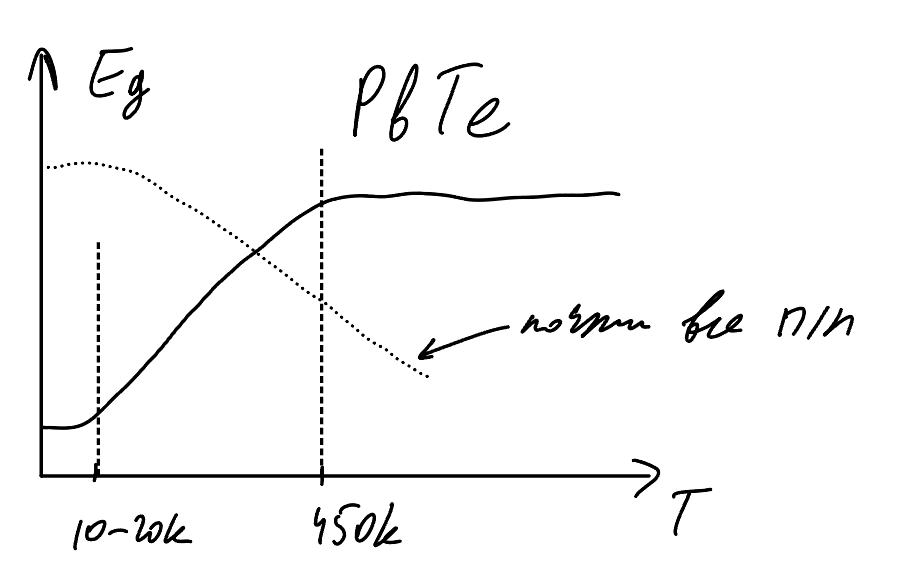
\includegraphics[width=0.45\textwidth]{phys_8_10}}
    \subfigure{
    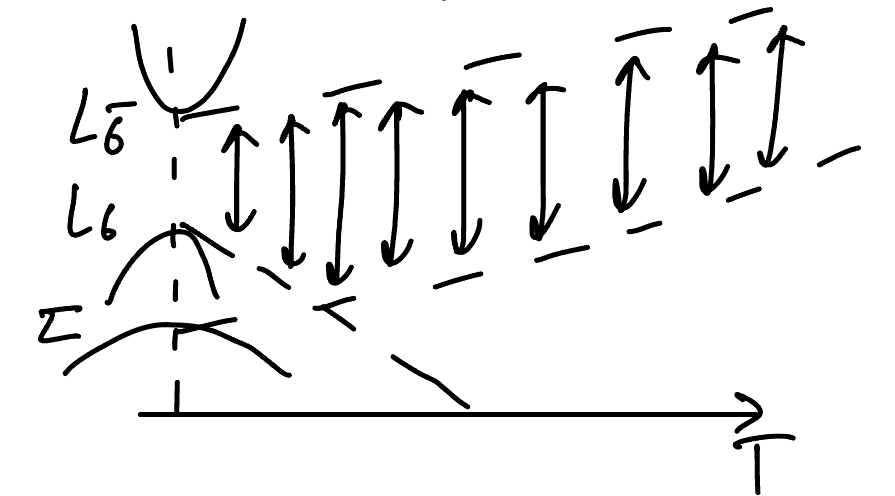
\includegraphics[width=0.45\textwidth]{phys_8_11}}
\end{figure}

Справа от весщелевого состояния $E_g \downarrow \uparrow T$, слева от бесщелевого сотояния $E_g \uparrow \uparrow T$.

Для полупроводников на основе свинца наблюдается рост с насыщением запрещённой зоны от температуры (для большинства других полупроводников с ростом температуры запрещённая зона уменьшается). С ростом температуры края зон $L{6}$ и $L_{\bar{6}}$ расходятся (увеличение запрещённой зоны), а край зоны $\Sigma$ движется вверх (приблизительно с такой же скорость, что и $L_6$). С некоторого момента зона $\Sigma$ оказывается выше $L{6}$ (выход на насыщение).

До точки $x\leq 0,3$ можно использовать модифицированный закон Кейна ($\displaystyle E\left(1+\frac{E}{E_g}\right)=\frac{\hbar^2 k_\perp^2}{2 m_t^*(0)}+\frac{\hbar^2 k_\parallel^2}{2 m_l^*(0)}$, 2 параметра $m_t$ и $m_l$).

Далее лучше закон дисперсии Диммака ($\left(\frac{E_g}{2}+\frac{p_\perp^2}{2 m_t^{-}}+\frac{p_\parallel^2}{2 m_t^{-}}-E\right)\left(-\frac{E_g}{2}-\frac{p_\perp^2}{2 m_t^{+}}-\frac{p_\parallel^2}{2 m_t ^+}-E\right)=E_\perp \frac{p_\perp^2}{2 m}+E_\parallel \frac{p_\parallel^2}{2 m}$, $m_t^{ \pm}$, $m_l^{ \pm}$, $E_\perp$, $E_\parallel$ ---  6 параметров, определяются только экспериментально).


\begin{figure}[h!]
    \centering
    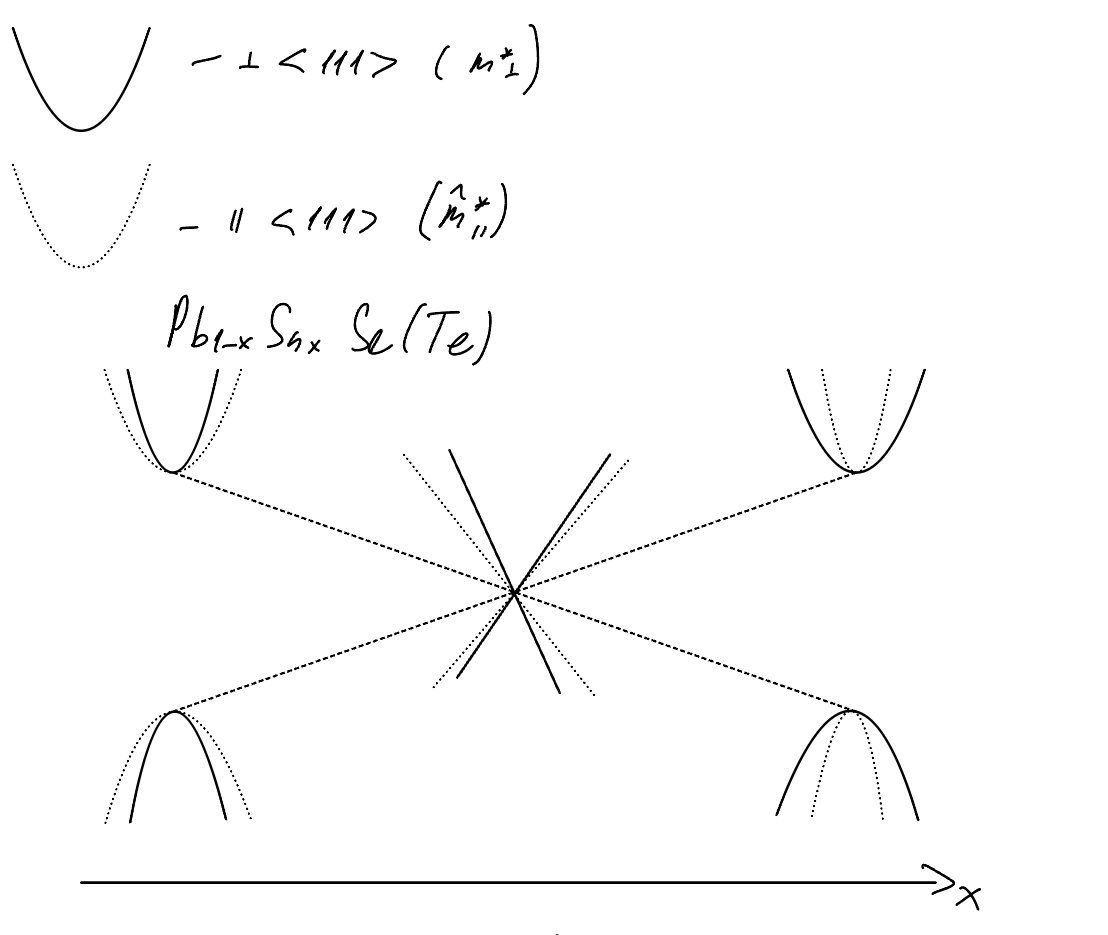
\includegraphics[width=0.6\textwidth]{phys_8_12}
\end{figure}

\section{Прямой и инверсный спектры Кейна для полупроводников $A^3B^5$ и $A^2B^6$.}

\textbf{Зонная структура $A^3B^5$}

A: In, Ga, Al...

B: Sb, As, P, N...

Общая (наиболее распространённа)я ситуация

\begin{enumerate}
    \item Кристаллическая решётка типа сфалерита (цинковой обманки)
    \item Зона Бриллюэна --- кубооктаэдр
    \item Закон дисперсии Кейна:

    $$\left\{ \begin{array}{c}
        E_c=E_g+\frac{1}{2} E_g \left( \sqrt{1+\frac{8k^2P^2}{3E_g^2}} -1  \right) \\
        E_{v_1} = -\frac{\hbar^2 k^2}{2m}\\
        E_{v_2} = -\frac{E_g}{2}\left( \sqrt{1+\frac{8k^2P^2}{3E_g}} -1 \right)\\
        E_{v_3} = -\Delta - \frac{P^2k^2}{3(E_g+\Delta)}
    \end{array} \right.$$
    
    $\Delta$ --- энергия спинорбитального взаимодествия, $P=\frac{\hbar}{m} \int U^*_c \hat{\bar{p}} U_{v_2} d\bar{r}$ --- матричный элемент оператора импульса ($\hat{\bar{p}}=-i\hbar \nabla$), $U_c$, $U_{v_2}$ --- блоховские амплитуды.
    
    Неквадратичный закон для электронов и лёгких дырок (зоны проводимости и лёгких дырок зеркальны ($m_c^*=m_{v_2}^*$)).
    
    При выборе начала отсчёта на уровне Ферми закон превращается в $E\left(1+\frac{E}{E_g}\right)=\frac{2 k^2 p^2}{3 E_g} \leftrightarrow \frac{\hbar^2 k^2}{2 m^*}$. В узкощелевых полупроводниках необходимо учитывать вклад $1+\frac{E}{E_g}$, эффективная циклотронная масса  $m^*_c(E)=m^*(0)(1+\frac{2E}{E_g})$.
\end{enumerate}

\begin{figure}[h!]
    \centering
    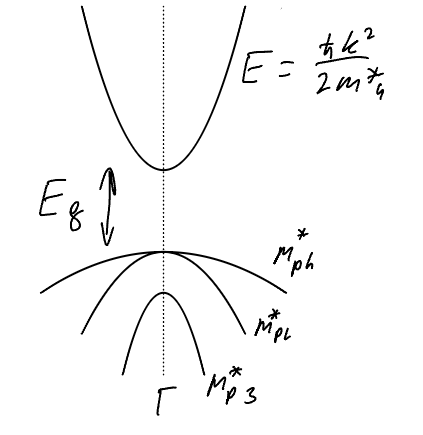
\includegraphics[width=0.4\textwidth]{phys_8_2}
\end{figure}

Отклонение от этой системы:

\begin{itemize}
    \item GaN, InN, AlN кристаллизуются в решётки вюрцита (ГПУ)
    \item Наличие у ряда полупроводников дополнительных экстремумов в зоне проводимости
\end{itemize}

\begin{figure}[h!]
    \centering
    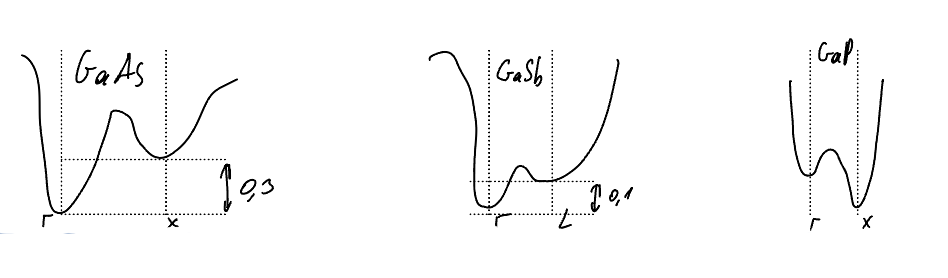
\includegraphics[width=0.8\textwidth]{phys_8_3}
\end{figure}

\begin{figure}[h!]
    \centering
    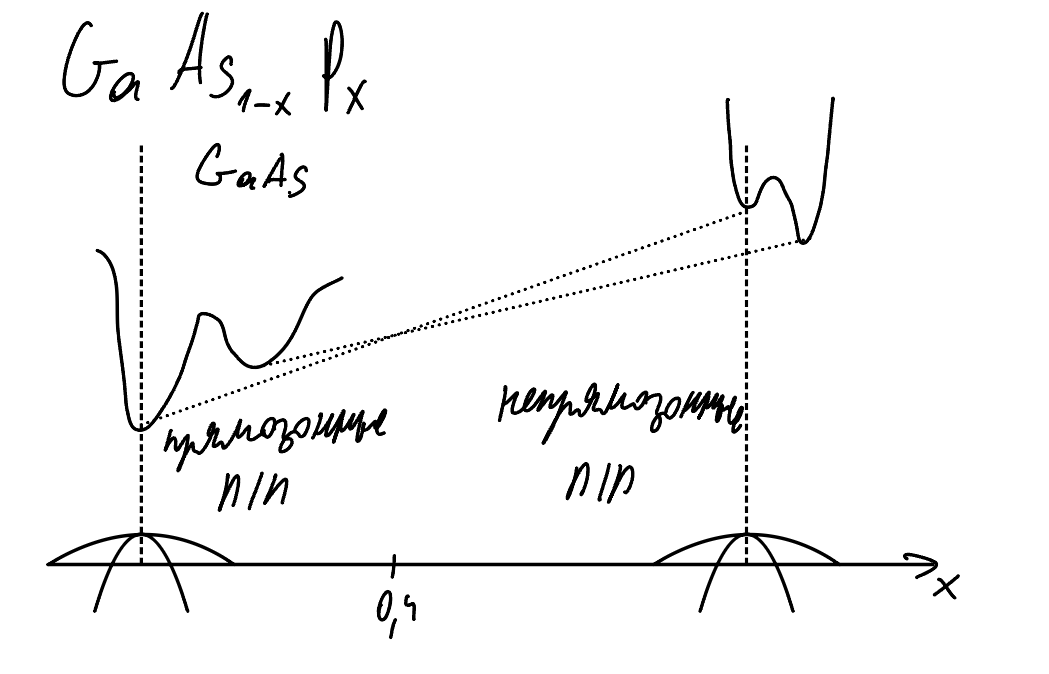
\includegraphics[width=0.7\textwidth]{phys_8_4}
\end{figure}

Прямозонные используются в оптике.


\textbf{Зонная структура $A^2B^6$}

A: Zn, Cd, Hg...

B: O, Se, S, Te...

\begin{enumerate}
    \item Кристаллическая решётка типа сфалерита или вюрцита
    \item Зона Бриллюэна --- кубооктаэдр
    \item Выполняется закон Кейна
\end{enumerate}

Особенности полупроводников на основе Hg:

\begin{enumerate}
    \item При низких температурах существуют свободные носители заряда (как в металлах)
    \item Инверсная зонная структура ($E_g<0$ в законе Кейна)
\end{enumerate}

\begin{figure}[h!]
    \centering
    \subfigure{
    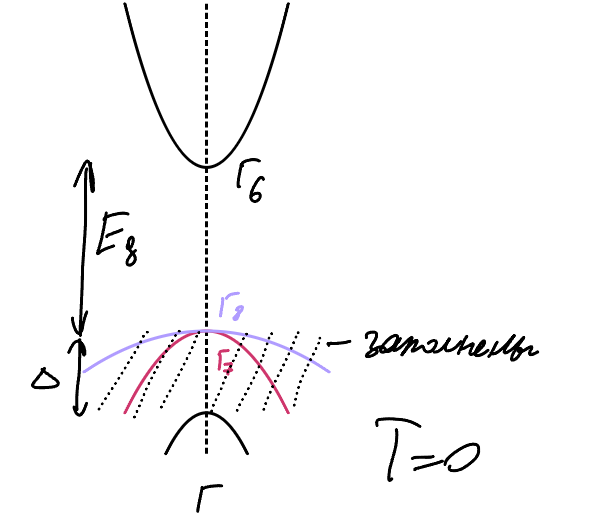
\includegraphics[width=0.4\textwidth]{phys_8_5}}
    \subfigure{
    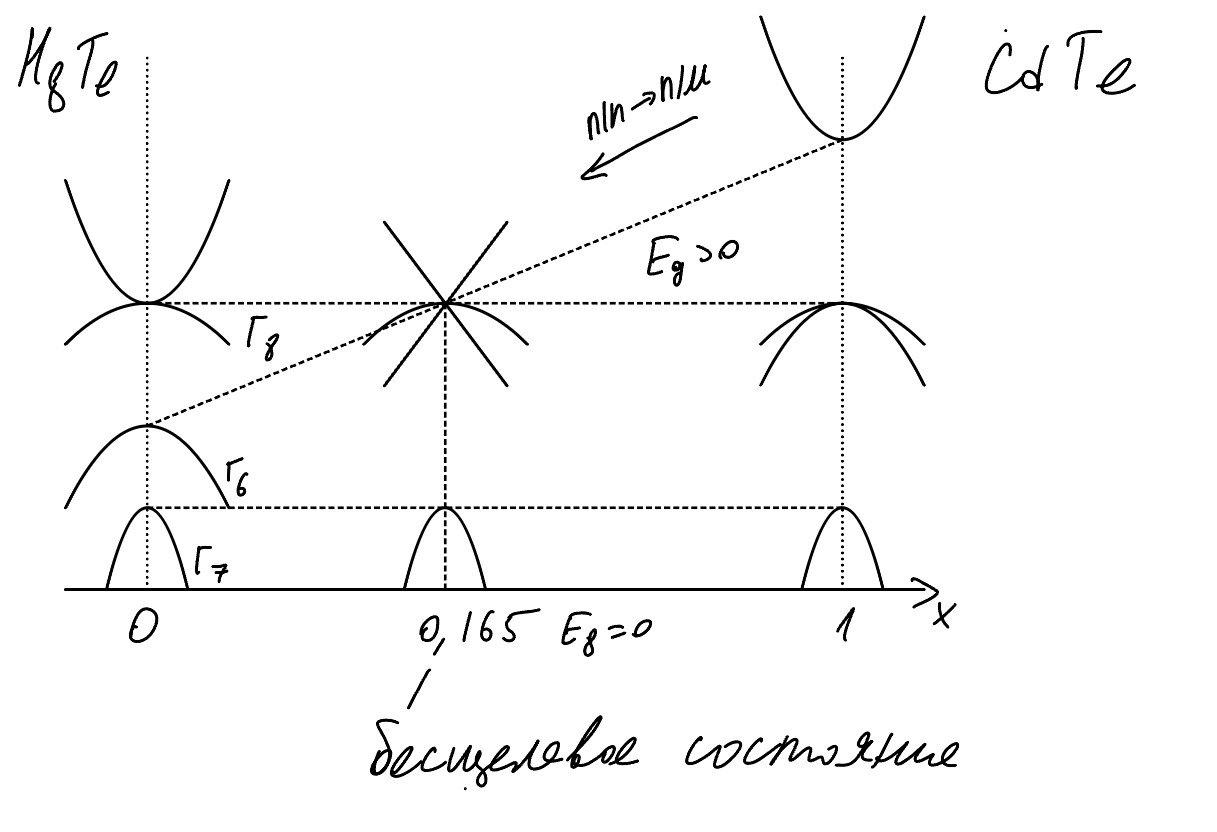
\includegraphics[width=0.5\textwidth]{phys_8_6}}
\end{figure}


$\displaystyle E=\frac{E_g}{2}\left(\sqrt{1+\frac{8 k^2 p^2}{3 E_g^2}}-1\right) \underset{E_g=0}{\longrightarrow} \quad E=\sqrt{\frac{2}{3}} pk$ --- Линейный закон дисперсии (как у графена. Обладает нулевой запрещённой зоной).

\section{Энергетические уровни дефектов в полупроводниках. Водородоподобная модель примеси. Примесные зоны.}

\textbf{Собственная проводимость.}

Собственный полупроводник --- полупроводник без дефектов и примесей.

При $T=0$ проводимость нулевая. При повышении температуры появляются свободные электроны (возникает проводимость $\sigma = e \mu n$). На место ушедшего электрона может придти электрон из соседней связи. Разорванная связь --- дырка тоже вносит вклад в проводимость. Концентрация электронов и дырок одинакова $\sigma = e \mu n + e \mu p$. Механизм проводимости --- по незаполненным связям.

\begin{figure}[h!]
    \centering
    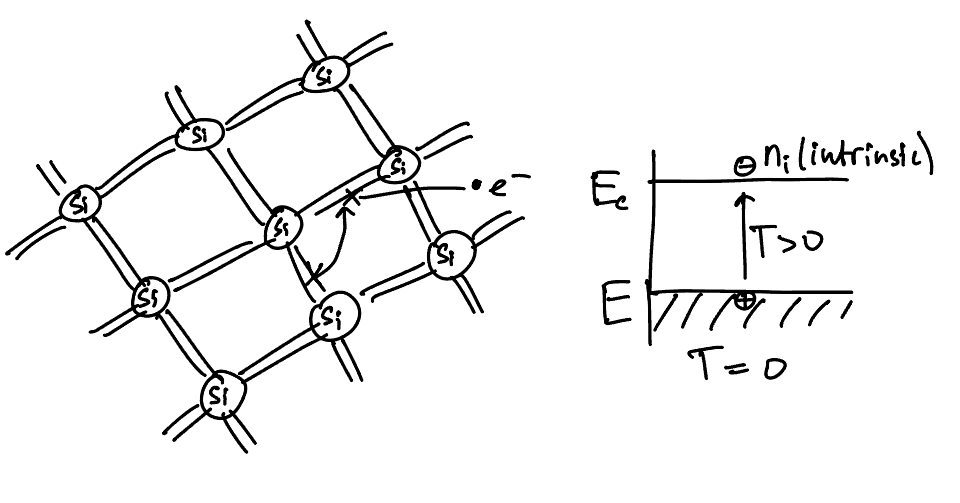
\includegraphics[width=0.5\textwidth]{intrinsic}
\end{figure}

\textbf{Примесная проводимость}

\textit{Донорный полупроводник (n-тип)}

\begin{figure}[h!]
    \centering
    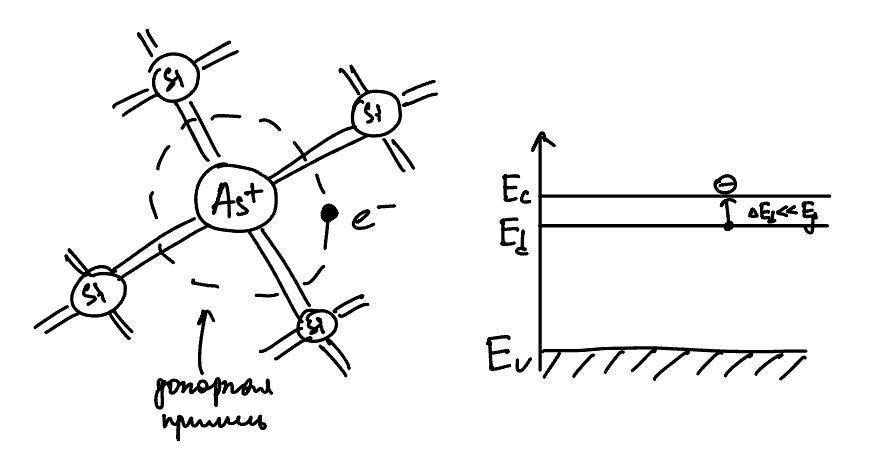
\includegraphics[width=0.5\textwidth]{Donor}
\end{figure}

При $T=0$ электрон связан с атомом примеси и не вносит вклад в проводимость. С ростом температуры всё больше ёлетронов покидают атом примеси и начинают движение по решётке. В этом случае проводимость только электронная.

\textit{Акцепторный полупроводник (p-тип)}

\begin{figure}[h!]
    \centering
    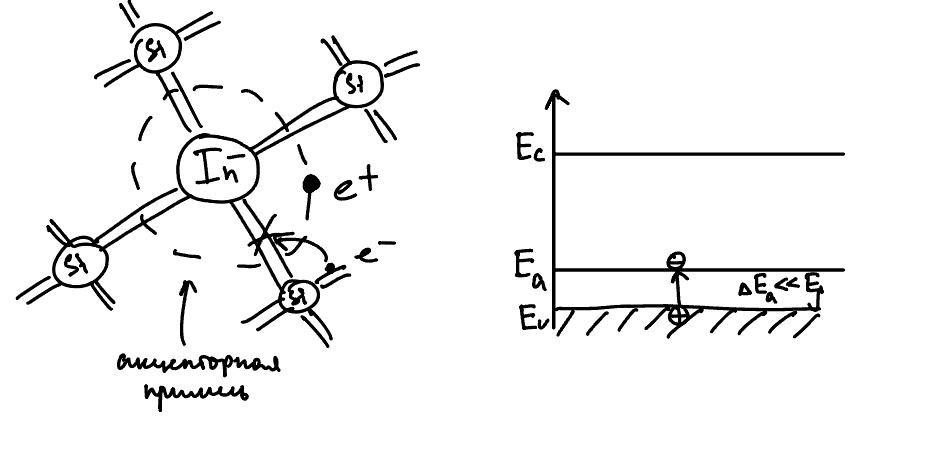
\includegraphics[width=0.5\textwidth]{Acceptor}
\end{figure}

При лигировании примесью с меньшим количеством валентных электронов, чем у основного атома одна связь остаётся незаполненной. На эту связь могут перемещаться электроны с другой (перемещая незаполненную связь по кристаллу) --- осуществляется дырочная проводимость.

\textbf{Примесные зоны. Классификация по степени лигирования.}

\begin{figure}[h!]
    \centering
    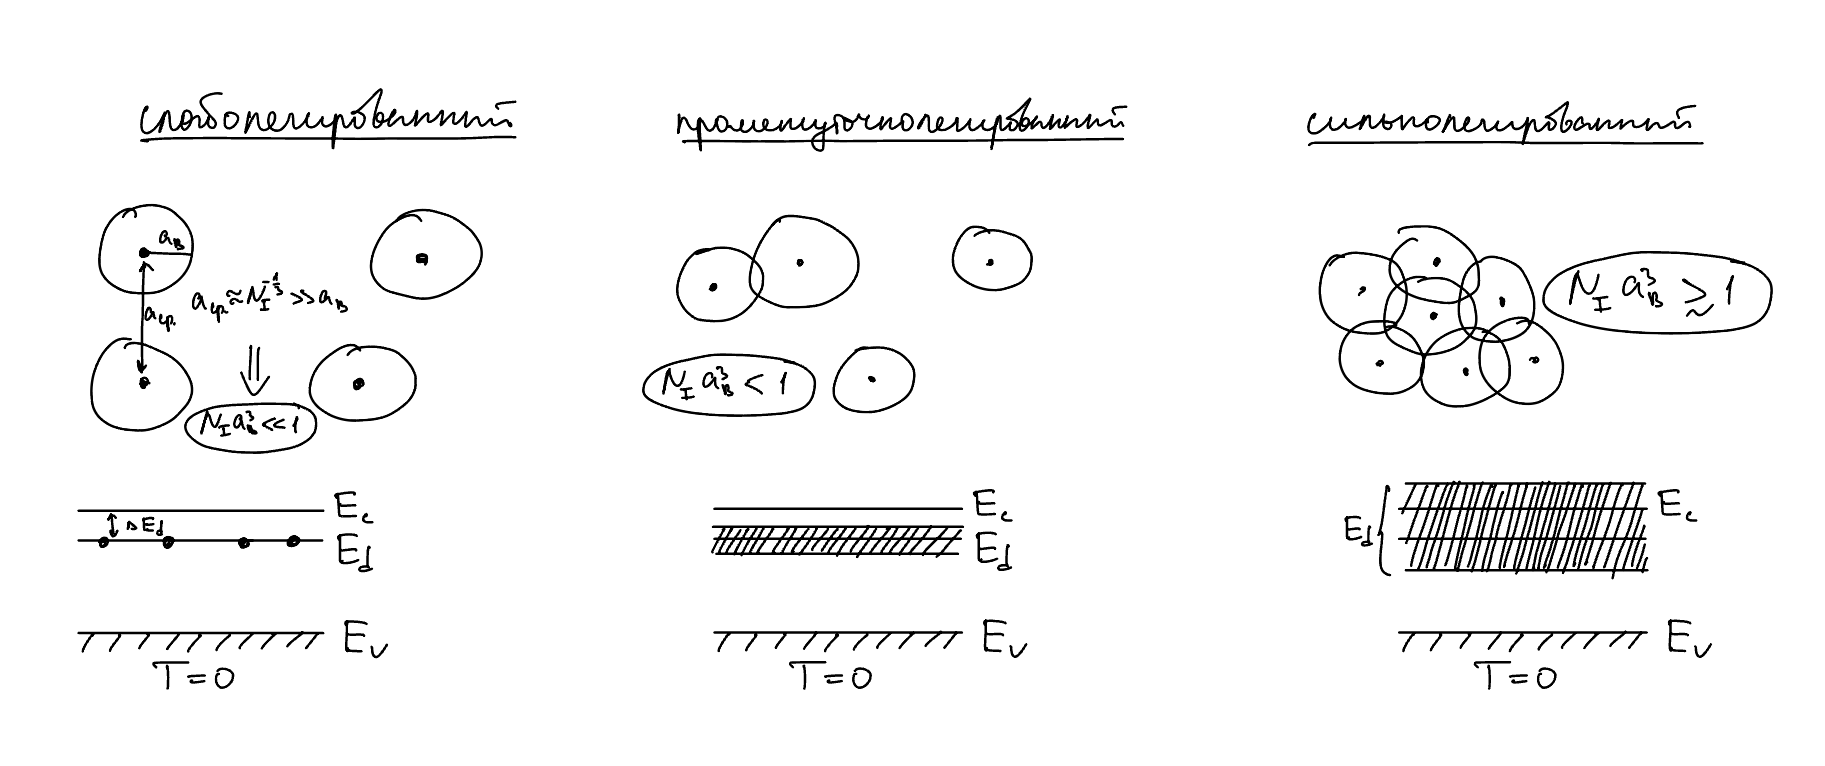
\includegraphics[width=0.95\textwidth]{prim}
\end{figure}

\begin{enumerate}
    \item Слабое лигирование. Среднее расстояние между примесями много больше боровского радиуса. Примеси не взаимодействуют.
    \item Среднее лигирование. Среднее расстояние порядка боровского радиуса, примеси взаимодействую. Перекрытие волновых функций электронов соседних примесей приводит к размытию уровней в зоны.
    \item Волновые функции электронов примесей сильно перерываются, примесная зона может достигать зоны проводимости и перекрываться с ней. Сильнолигированный полупроводник похлж на металл.
\end{enumerate}

Появление дефектов --- появление локальных уровней на фоне зонной структуры полупроводника. Нахождение уравнений дефектов --- решение уравнения Шрёдингера с потенциалом дефекта $V(\bar{\epsilon})$

$$
\left\{\frac{-\hbar^2}{2 m} \nabla^2+U(\bar{r})+V(\bar{r})\right\} \Psi(\bar{r})=E \psi(\bar{r})
$$

$\psi(\bar{r})$ --- волновая функция в окрестности дефекта, $\Psi(\bar{r})=\sum_{\bar{n}^{\prime} ; \bar{k^{\prime}}} C_{n^{\prime}}\left(\bar{k}^{\prime}\right) \psi_{n^{\prime} k^{\prime}}(\bar{r})$, $\bar{n}^{\prime}$ --- номер зоны, $\bar{k^{\prime}}$ --- точки в зоне Бриллюэна.

Задача не имеет общего решения. Выделяется самый простой возможный случай, в котором можно получить конечное решение: водородоподобная модель.

$$\Psi(\bar{v}) \sim \psi_{n, \bar{k}_0}(\bar{r})$$

\noindent $k_0$ --- точка экстремума зоны Бриллюэна.

$V(\bar{r})=\frac{e^2}{4 \pi \varepsilon \varepsilon_0 r}$

$$
\left\{\begin{array}{l}
\Delta E_d=\frac{13,6}{\varepsilon^2}\left(\frac{m^*}{m}\right) \frac{1}{n^2} \\
a_B=0,53 \frac{\varepsilon}{z}\left(\frac{m}{m^*}\right) n^2
\end{array}\right.
$$


\begin{enumerate}
    \item Случай <<мелких>> уровней $V(\bar{r})$ --- дальнодействующий потенциал. $\Delta x \Delta p \geq \hbar \Rightarrow \Delta x \Delta k \geq 1$, $\Delta x = a_B \gg a \Rightarrow \Delta k \ll 1/a$ (подходит для описания примесных уровней $Si$, $Ge$, $A^3B^5$, $A^2B^6$)
    
    \begin{figure}[h!]
        \centering
    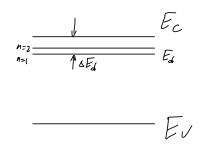
\includegraphics[width=0.3\textwidth]{phys_10_1}
    \end{figure}

    \item Альтернативный случай --- <<глубокие>> уровни. В этом случае учитываются многие энергетические зоны и все точки зоны Бриллюэна. Реализуется при: $V(\bar{r})$ --- короткодействующий, $\Delta E_t \approx E_g$. $|Delta x \leq a \Rightarrow \Delta k \sim \Delta k_\text{З.Бр.}$
    \item Резонансные уровни --- уровни расположение на фоне разрешённых зон: возможны переходы электронов с уровня в зону и обратно из-за этого уширение уровня дефектов ($\Delta E \Delta t \geq \hbar$). Резонансные уровни могут быть как мелкими так и глубокими.
\end{enumerate}

\begin{figure}[h!]
    \centering
    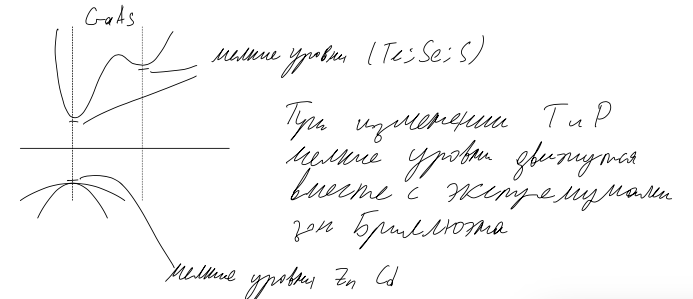
\includegraphics[width=0.7\textwidth]{phys_10_2}
\end{figure}

Глубокие уровни образованы всеми точками зон Бриллюэна, они не могут следовать за какой-то конкретной.

\begin{figure}[h!]
    \centering
    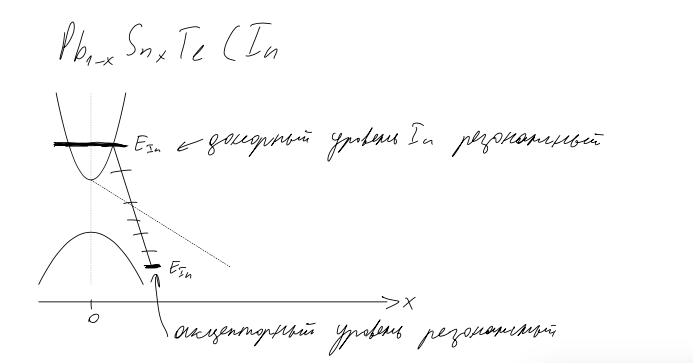
\includegraphics[width=0.7\textwidth]{phys_10_3}
\end{figure}

\section{Уравнение электронейтральности. Статистика носителей заряда в полупроводнике с одним типом примеси.}

Из расчёта известно $n=N_c F_{1/2}(\eta)$, $p=N_v F_{1/2}(\eta - \Delta\varepsilon)$.

\noindent где $F_{1/2}$ --- интеграл Ферми, $\frac{E-E_{c}}{kT}=\varepsilon$ --- энергия электронов относительно дна зоны проводимости, $\frac{E_g}{kT}=\Delta \varepsilon$, $\frac{F-E}{kT}=\eta$, $F$ --- уровень Ферми, $N_{с}$ $N_{v}$ --- функции плотности состояний в зоне проводимости и в валентной зоне. Но не известно значение уровня Ферми. Цель введения закона электронейтральности --- расчет $F(T)$.

Суть (физический смысл): кристалл в целом электронейтрален, хотя состоит из заряженных частиц. $\sum \limits_i N_{-} = \sum \limits_i N_{+}$.

\begin{figure}[h!]
    \centering
    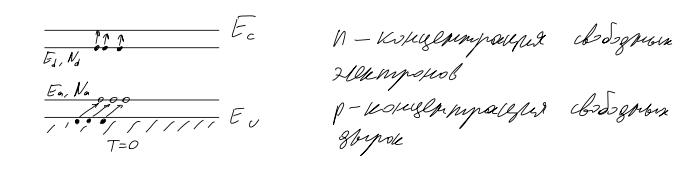
\includegraphics[width=0.9\textwidth]{phys_11_1}
\end{figure}

$N_d$ --- концентрация атомов донорной примеси
$N_a$ --- концентрация атомов акцепторной примеси
$n_d$ --- концентрация электронов на донорном уровне ($E_d$)
$p_d$ --- концентрация дырок на донорном уровне ($E_d$)
$n_a$ --- концентрация электронов на акцепторном уровне ($E_a$)
$p_a$ --- концентрация дырок на акцепторном уровне ($E_a$)
$N_d^+$ --- концентрация ионов донорной примеси
$N_a^-$ --- концентрация ионов акцепторной примеси

$$
\left\{\begin{array} { l } 
{ N _ { d } ^ { + } = p _ { d } } \\
{ N _ { a } ^ { - } = n _ { a } }
\end{array} \quad \left\{\begin{array}{l}
n_d+p_d=N_d \\
n_a+p_a=N_a
\end{array}\right.\right.
$$

Каждый примесный уровень может быть занят либо электроном, либо дыркой ($N_a^-=N_a-p_a$, $N_d^+=N_d-n_d$)

Уравнение электронейтральности: $n+N_a-p_a=p+N_d-n_d$ (можно обобщить для нескольких типов примеси $n+\sum n_d-p-\sum p_a=\sum N_d-\sum N_a$).

\textbf{Статистика полупроводника с одним типом примеси}

Из уравнения электронейтральности следует, что $n=N_d-n_d+p=p_d+p$.

Предположения:

\begin{itemize}
    \item невырожденный полупроводник $n=N_ce^\eta$, $p=N_ve^{-\eta-\Delta\varepsilon}$
    \item Мелкие примеси $\Delta E_d \ll E_g$ (это позволит разбить шкалу температур на характерные уровни)
\end{itemize}

\begin{figure}[h!]
    \centering
    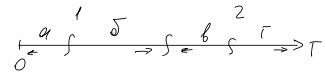
\includegraphics[width=0.5\textwidth]{phys_11_3}
\end{figure}

1 --- область низких температур, в которой происходит ионизация только атомов примеси.
2 --- область высоких температур, в которой происходит ионизация атомов основного вещества.

1. Ионизация только примеси $\Rightarrow p=0 \Rightarrow n=p_d$.

$$\displaystyle p_d=\frac{N_d}{ge^{\frac{F-E_d}{kt}}+1} = \frac{N_d}{g e^{g+\varepsilon_d}+1}$$

%\vspace{0.5cm}

$$\displaystyle \frac{F-E_c}{kT} = \eta, \; \frac{E_c-E_d}{kT}=\frac{\Delta E_d}{kT} = \varepsilon_d, \; n=N_c e^\eta, \; e^\eta = \frac{n}{N_c}$$

$$n=\frac{N_{d}}{g \frac{n}{N_c} e^{\varepsilon_d}+1}$$

$$n^2+\underbrace{\frac{N_c}{g} e^{-\varepsilon d}}_a n \underbrace{-\frac{N_c N_d}{g} e^{-\varepsilon_d}}_c=0$$

$$x^2+ax+c=0$$

$$x=\frac{a}{2}\left( \pm \sqrt{1-\frac{4 c}{a^2}}-1\right)$$

$$
n=\frac{N_c}{2 g} e^{-\varepsilon_d}\left[ \pm \sqrt{1+\frac{4 g N_d}{N_c} e^{\varepsilon_d}}-1\right]
$$

\vspace{2cm}

а) $\displaystyle \frac{4gN_d}{N_c} e^{\varepsilon _d} \gg 1, \; \varepsilon_d \sim \frac{1}{T}, \; N_c \sim T^{3/2}$

\vspace{0.5cm}

Случай низких температур в области 1

$$
n \approx \frac{N_c}{2 g} e^{-\varepsilon_d} \sqrt{\frac{4 g N_d}{N_c} e^{\varepsilon_d}}=\sqrt{\frac{N_c N_d}{g}}e^{-\frac{-\varepsilon_d}{2}} = \sqrt{\frac{N_c N_d}{g}}e^{-\frac{E_c - E_d}{2kT}}
$$

Рост $n$ с увеличением $T$ --- 1а область примесной ионизации.

$$F(T) = \frac{E_c+E_d}{2} + \frac{kT}{2} \ln \frac{N_d}{g N_c}$$
\vspace{2cm}

б) $\displaystyle \frac{4 g N_d}{N_c} e^{\varepsilon_d} \ll 1 \quad\left(\sqrt{1+x} \approx 1+\frac{x}{2} \quad x<1\right)$

\vspace{0.5cm}

$$
n \approx \frac{N_c}{2 g} e^{-\varepsilon_d}\left\{1+\frac{2g N_d}{N_c} e^{\varepsilon_d}-1\right\}
$$

б --- область истощения (насыщения примеси)

$$
n=N_c e^{\frac{F-E_c}{k T}}=N_d
$$

$$
F(T)=E_c-k T \ln \frac{N_d}{N_c}
$$

\vspace{2cm}

2. $\displaystyle n=\frac{n_i^2}{n}+N_d$

\vspace{0.5cm}

$$
n^2-N_d n-n_i^2=0
$$

$$
n=\frac{N_d}{2} \pm \sqrt{\frac{N_d^2}{4}+n_i^2}
$$

\vspace{2cm}
в) $\displaystyle \frac{N_d^2}{4} \gg n_i^2, \; n=\frac{N_d}{2}+\frac{N_d}{2}=N_d$ --- всё ещё область истощения примеси.

\vspace{2cm}
г) $\displaystyle \frac{N_d^2}{4}<<n_i^2, n \rightarrow n_i(T)$ --- интервал собственной ионизации. Поведение аналогично собственному полупроводнику.
\vspace{0.5cm}

\begin{figure}[h!]
    \centering
    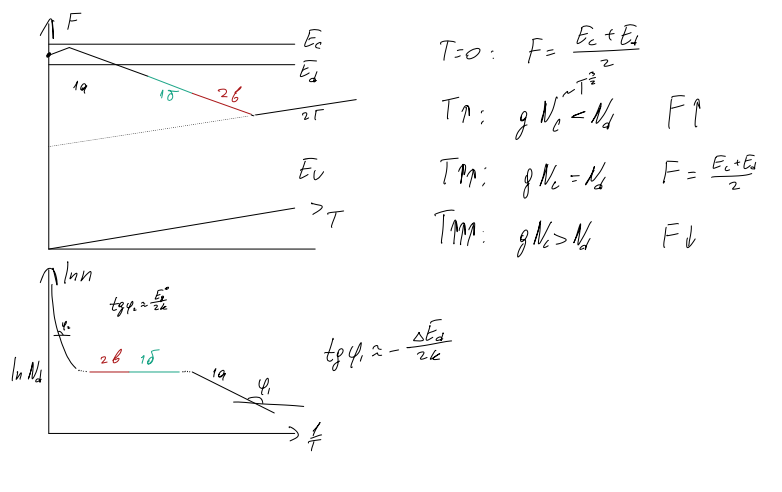
\includegraphics[width=0.85\textwidth]{phys_11_4}
\end{figure}


\begin{figure}[h!]
    \centering
    \subfigure{
    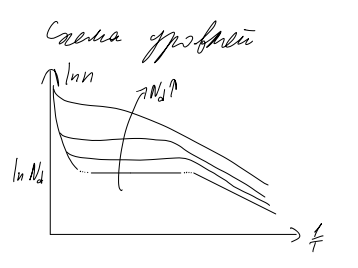
\includegraphics[width=0.4\textwidth]{phys_11_5}}
    \subfigure{
    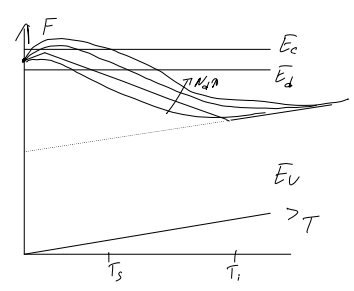
\includegraphics[width=0.5\textwidth]{phys_11_6}}
\end{figure}

$T_s$, $T_i$ --- нижняя и верхняя температура истощения.
\clearpage

\section{Неравновесные носители заряда (время жизни, механизмы рекомбинации). Уравнение непрерывности и примеры его использования.}

Неравновесные носители заряда возникают из-за:

\begin{enumerate}
    \item Внешних воздействий 
    \begin{enumerate}
        \item Облучение квантами электромагнитного излучения
        \item Облучение быстрыми частицами (электроны, нейтроны, $\gamma$-излучение)
        \item Приложение электрического поля 
        \item Ток в p-n-переходе
    \end{enumerate}
    \item Внутренних воздействий
    \begin{enumerate}
        \item Изменение температуры
    \end{enumerate}
\end{enumerate}

% \textbf{Неравновесная функция распределения}

% $$
% n(T)=\int f_n(E ; T) N_c(E) d E \approx \int \frac{N_c(E)}{e^{\frac{E-F_n}{kT}}+1} d E=N_c F_{1/2}\left(\eta_n\right)
% $$

% $$
% p(T)=\int f_p(E ; T) N_v(E) d E \approx \int \frac{N_v(E)}{e^{\frac{E-F_p}{kT}}+1} d E=N_v F_{1/2}\left(-\eta_p - \Delta \varepsilon \right)
% $$

% $f_n$, $f_p$ --- в общем виде не известны
% $F_n$, $F_p$ --- квазиуровни Ферми
% $\eta_n$, $\eta_p$ --- приведённые безразмерные квазиуровни Ферми


\textbf{Время жизни}


Простая механическая модель: 1 тип электронов l механизмов рекомбинации. $W_{nl}=S_{nl}P_l \langle V_{nl} \rangle$ ($\left[ \frac{1}{\text{см}} \right] = \left[ \text{см}^2 \text{см}^{-3} \frac{\text{см}}{\text{с}} \right]$) --- вероятность рекомбинации электронов по механизму l.

$S_{nl}$ --- эффективное сечение процесса рекомбинации электронов по механизму l.

$\frac{1}{W_{nl}}=\tau_{nl}$ --- среднее время жизни электрона при рекомбинации по механизму l.

$W_n=\sum \limits_l W_{nl} \quad \frac{1}{\tau_n} = \sum \limits_l \frac{1}{\tau_{nl}}$ 

\textbf{Основные механизмы рекомбинации}

1) По типу переходов 

а) Межзонная рекомбинация 

\begin{figure}[h!]
    \centering
    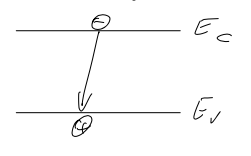
\includegraphics[width=0.3\textwidth]{phys_12_1}
\end{figure}

б) Рекомбинация через рекомбинационные уровни

\begin{figure}[h!]
    \centering
    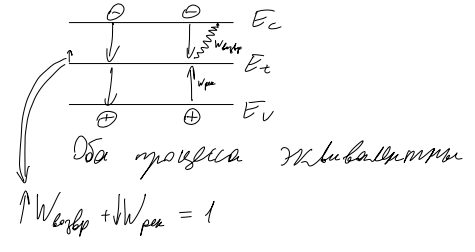
\includegraphics[width=0.3\textwidth]{phys_12_2}
\end{figure}

в) Экситонная рекомбинация

г) Поверхностная рекомбинация

\pagebreak
2) По виду выделяемой энергии

а) Межзонная рекомбинация (излучательная)
\begin{figure}[h!]
    \centering
    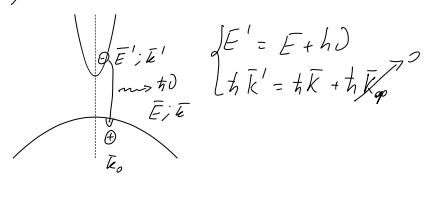
\includegraphics[width=0.3\textwidth]{phys_12_3}
\end{figure}


б) Безизлучательная рекомбинация 

\begin{figure}[h!]
    \centering
    \includegraphics[width=0.3\textwidth]{phys_12_4}
\end{figure}

-- Фононная (вся энергия идёт на создание фонона)

\begin{figure}[h!]
    \centering
    \includegraphics[width=0.3\textwidth]{phys_12_5}
\end{figure}

-- Ударная (Оже) рекомбинация

\begin{figure}[h!]
    \centering
    \includegraphics[width=0.3\textwidth]{phys_12_6}
\end{figure}

\textbf{Уравнение непрерывности и примере его использования}

В выделенном объеме концентрация носителей заряда может меняться за счет генерации, рекомбинации, диффузии и дрейфа.

$$
\frac{d n}{d t}=\overbrace{g_{n E}-r_{n E}}^{G_n}+\overbrace{g_{n I}-r_{n I}}^{-R_n}+\frac{1}{e} \text { div } \bar{j}_n(r)
$$

$$
\frac{d p}{d t}=\overbrace{g_{p E}-r_{p E}}^{G_p}+\overbrace{g_{p I}-r_{p I}}^{-R_p}-\frac{1}{e} \text { div } \bar{j}_p(r)
$$

$g$ --- скорость генерации носителей заряда
$r$ --- скорость рекомбинации носителей заряда
$G_{n,p}$ --- эффективная скорость генерации
$R_{n,p}$ --- эффективная скорость рекомбинации
$E$ --- внешние
$I$ --- внитренние

\textit{Рекомбинация при монополярной генерации (линейная рекомбинация)}

Предположения:

\begin{enumerate}
    \item Выключаем генерацию в момент времени t=0
    \item Полупроводник однородный ($n(\bar{r})=const, \; \bar{E}=0$)
    \item $\Delta \ll n_0$ --- условие низкоуровневого возбуждения (инжекции)
    \item Генерация примесная
\end{enumerate}

$$
\frac{d n}{d t}= \overbrace{G_n}^{0}-R_n+\overbrace{\frac{1}{e} \mathrm{div}\bar{j}_n}^0 \Rightarrow \frac{d n}{d t}=-W_n \Delta n=-\frac{\Delta n}{\tau_\text{ж}}
$$

$$
\Delta n(t)=\Delta n(0) e^{-\frac{t}{\tau_\text{ж}}}, \quad n=n_0+\Delta n
$$

$\tau_\text{ж}$ --- время за которое значение $\Delta n$ уменьшится в $e$ раз.


\begin{figure}[h!]
    \centering
    \subfigure{
    \includegraphics[width=0.6\textwidth]{phys_12_7}}
    \subfigure{
        \includegraphics[width=0.3\textwidth]{phys_12_8}}
\end{figure}


\textit{Рекомбинация при биполярной генерации (квадратичная рекомбинация)}

Предположения:

\begin{enumerate}
    \item Выключаем генерацию в момент времени t=0
    \item Полупроводник однородный ($\bar{E}=0$)
    \item Межзонная генерация ($\Delta n = \Delta p$)
    \item Уровень возбуждения любой
\end{enumerate}

$\frac{d n}{d t}=\frac{d p}{d t}=-R_n=-\gamma\left(n p-n_0 p_0\right)$, $\gamma$ --- коэффициент межзонной рекомбинации.

$\left.\begin{array}{l}n=n_0+\Delta n \\ p=p_0+\Delta p\end{array}\right\} \rightarrow-\gamma\left(n p-n_0 p_0\right)$

$\displaystyle \frac{d n}{d t}=-\gamma\left(n_0 p_0+n_0 \Delta p+p_0 \Delta n+\Delta n \Delta p-n_0 p_0\right)$ 

$\displaystyle \frac{d n}{d t}=-\gamma\left(n_0 \Delta p+p_0 \Delta n+\Delta n \Delta p\right)$

\vspace{0.5cm}

а) Низкий уровень инжекции ($\Delta n, \Delta p \ll n_0, p_0$)

-- p-тип ($p_0\gg n_0$), $\frac{d(\Delta n)}{d t}=-r p_0 \Delta n \sim \Delta n$

$\Delta n(t)=\Delta n(0) e^{-\frac{t}{\tau_n}}, \tau = \frac{1}{\gamma p_0}$

-- n-тип ($n_0\gg p_0$), $\frac{d(\Delta n)}{d t}=-r n_0 \Delta p \sim \Delta p$

$\Delta p(t)=\Delta p(0) e^{-\frac{t}{\tau_p}}, \tau=\frac{1}{\gamma n_0}$

Времена жизни в процессах определяется концентрацией неосновных носителей заряда.

б) Высокий уровень инжекции ($\Delta n, \Delta p \gg n_0, p_0$)

$\frac{d(\Delta n)}{d t}=\frac{d(\Delta n)}{d t}=-\gamma(\Delta n)^2 \sim(\Delta n)^2$ --- квадратичная рекомбинация.

$\frac{d(\Delta n)}{(\Delta n)^2}=-\frac{d t}{\gamma} \rightarrow \frac{1}{\Delta n}=\gamma t+C$. Граничное условие $t=0, \Delta n=\Delta n(0) \Rightarrow C=\frac{1}{n(0)}$

$\Delta n(t)=\frac{\Delta n(0)}{1+\gamma \Delta n(0) t}$

Не можем вывести всего один параметр ($\tau_n$ --- время жизни), который характеризует весь процесс.

Мнгновенное время жизни (обобщение $\tau_n$).

$$
\frac{d n}{d t}=-\frac{\Delta n(t)}{\tau_n(t)} \rightarrow \tau_n=-\frac{\Delta n(t)}{\frac{d n}{d t}}
$$


\begin{figure}[h!]
    \centering
    \subfigure{
    \includegraphics[width=0.3\textwidth]{phys_12_9}}
    \subfigure{
        \includegraphics[width=0.3\textwidth]{phys_12_10}}
        \subfigure{
        \includegraphics[width=0.3\textwidth]{phys_12_11}}
\end{figure}

\textit{Релаксация избыточной концентрации при конечном внешнем возбуждении}

Предположения:

\begin{enumerate}
    \item Включаем генерацию в момент времени t=0
    \item Полупроводник однородный ($\bar{E}=0$)
    \item Генерация монополярная
    \item Низкий уровень возбуждения
\end{enumerate}

$\frac{d n}{d t}=G_n-R_n$,  $R_n=\frac{\Delta n}{\tau _n}$

$$\frac{d(\Delta n)}{\Delta n-G_n \tau_n}=-\frac{d t}{\tau_n}$$

$$\ln \left(\Delta n-G_n \tau_n\right)=-\frac{t}{\tau_n}+C$$

$$\Delta n-G_n \tau_n=B e^{-\frac{t}{\tau_n}}$$

Граничные условия $t=0, \; \Delta n(t)=0 \Rightarrow -G_n\tau_n$

$$\Delta n(t)=G_n \tau_n\left[1-e^{-\frac{t}{\tau_n}}\right]$$

$$t \rightarrow \infty \quad \Delta n(t)=G_n \tau_n=\Delta n_\text{стац}$$

\begin{figure}[h!]
    \centering
    \includegraphics[width=0.8\textwidth]{phys_12_12}
\end{figure}

Прямоугольный импульс внешнего напряжения $\rightarrow$ искажённый импульс с наростаниями и спадами (фотоприёмники).

Большое время жизни $\Rightarrow$ большая амплитуда (хорошо), но затягивание спада (плохо).

\section{Контакт металл-полупроводник (контактная разность потенциалов, энергетические диаграммы, вольтамперная характеристика).}

\textbf{Полупроводник n-типа. $\Phi_\text{м}<\Phi_\text{п}$}

\begin{figure}[h!]
    \centering
    \includegraphics[width=0.9\textwidth]{phys_13_1}
\end{figure}

$$
\frac{d E}{d x}=\frac{\rho}{\varepsilon \varepsilon_0} \rightarrow \frac{d E}{d x}<0 \quad E>0
$$


$$
E=-\frac{d \varphi}{d x} \rightarrow \frac{d \varphi}{d x}<0 \quad \varphi>0
$$

$$
U=-e \varphi \rightarrow U<0
$$

\textbf{Полупроводник n-типа. $\Phi_\text{м}>\Phi_\text{п}$}


\begin{figure}[h!]
    \centering
    \includegraphics[width=0.9\textwidth]{phys_13_2}
\end{figure}

$$
E=\frac{e n_0}{\varepsilon \varepsilon_0}\left(L_0-x\right) \quad \varphi(x)=-\frac{e n_0}{2 \varepsilon \varepsilon_0}\left(L_0-x\right)
$$

Граничное условие: $x=0, \varphi(x)=-\varphi_k$

$$
-\varphi_k=-\frac{e n_0}{2 \varepsilon \varepsilon_0}\left(L_0\right)^2
$$

$\displaystyle L_0=\sqrt{\frac{2 \varepsilon \varepsilon_0 \varphi_k}{e n_0}}$ --- в сильном поле $e\varphi \gg kT$


Можно сравнить с $l_D$ в слабом поле $e\varphi \ll kT$ 

$$
l_D=\sqrt{\frac{\varepsilon \varepsilon_0 k T}{e^2 n_0}}
$$

При $T=300$~K $\varphi_k=1$~B, $\frac{L_0}{l_D}=10$


Для полупроводника p-типа аналогично (на рисунках показан уровень ферми такого полупроводника штрихом ($F_p$)).

\textbf{Энергетические диаграммы контакта металл-полупроводник во внешнем поле}

Рассмотрим контакт металл-полупроводник n-типа (с обеднённым слоем)

\begin{figure}[h!]
    \centering
    \subfigure{
    \includegraphics[width=0.6\textwidth]{phys_13_3}}
    \subfigure{
        \includegraphics[width=0.3\textwidth]{phys_13_5}}
\end{figure}

Изменится изгиб зон и толщина слоя ОПЗ (уменьшится при $U>0$, увеличится при $U<0$).

Напряжение приложено в прямом направление если металл +, а полупроводник -.

Токи при контакте: $$
j_{\text{ТП}}=A T^2 e^{-\frac{\Phi_\text{м}}{k T}}, \;
j_{\text{ТМ}}=A T^2 e^{-\frac{\Phi_\text{м} + e(\varphi_k+U)}{k T}}
$$

$$
j=j_{\text{ТП}}-j_{\text{ТМ}}=\underbrace{A T^2 e^{-\frac{\Phi_\text{м}}{k T}}}_{j_s}\left(e^{\frac{e U}{k T}}-1\right)
$$


$j_s$ --- ток насыщения.

\textbf{ВАХ}

\begin{figure}[h!]
    \centering
    \includegraphics[width=0.4\textwidth]{phys_13_4}
\end{figure}

Электроннодефецитный контакт металл-полупроводник --- диод Шоттки. Электронноизбыточный --- омический контакт (невыпрямляющий) применяется для исследования свойств полупроводников.

\section{Электронно-дырочный переход (энергетические диаграммы, идеальная ВАХ, ток насыщения).}

Предположения:

\begin{enumerate}
    \item Резкий p-n переход (концентрация примеси меняется скачком).
    \item Невырожденный полупроводник.
    \item Температура соответствует области истощения примеси.
    \item Использован один и тот же полупроводник, но с разными примесями.
\end{enumerate}

\begin{figure}[h!]
    \centering
    \includegraphics[width=0.85\textwidth]{phys_14_1}
\end{figure}

$\Phi_p > \Phi_n \Rightarrow j_\text{Tp}<j_\text{Tn}$

В обоих случаях заряд создают ионы примеси.

$\displaystyle e \varphi_k=\varphi_p-\varphi_n=\left(x+E_c-F\right)-\left(x+E_c-F\right)=F_n-F_p= \left(E_c-k T \ln \frac{N_c}{N_d}\right)-\left(E_v+k T \ln \frac{N_N}{N_a}\right)=-k T \ln \frac{n_i^2}{N_c N_v} -k T \ln \frac{N_c}{N_d}-k T \ln \frac{N_v}{N_a}=k T \ln \frac{N_c N_v}{n_i^2} \cdot \frac{N_d}{N_c} \cdot \frac{N_a}{N_v}= k T \ln \frac{N_d N_a}{n_i^2}$


$\displaystyle \varphi_k=\frac{k T}{e} \ln \frac{N_d N_a}{n_i^2} \quad e \varphi_k \leq E_g \quad \varphi_k \sim 1 B$

$$
n_i^2=N_c N_v e^{-\frac{E_g}{k T}} \rightarrow E_g=-k T \ln \frac{n_i^2}{N_c N_v}
$$


\textbf{Энергетические диаграммы p-n-перехода во внешнем поле}

\begin{figure}[h!]
    \centering
    \subfigure{
    \includegraphics[width=0.6\textwidth]{phys_14_2}}
    \subfigure{
    \includegraphics[width=0.3\textwidth]{phys_14_3}}
\end{figure}

\textbf{ВАХ}

$j_D$, $j_E$ --- Диффузионный ток и дрейфовый (дрейфовый ток не преодолевает энергетический барьер) соответственно.

$$
j=\underbrace{\left(\bar{j}_{D_p}+\bar{j}_{E_p}\right)}_0 + \underbrace{\left(\bar{j}_{D_n}+\bar{j}_{E_n}\right)}_0=0
$$

$$
j_E=j_{E_n}+j_{E_p}, \quad j_D=j_{D_n}+j_{D_p}
$$

\begin{figure}[h!]
    \centering
    \includegraphics[width=0.4\textwidth]{phys_14_4}
\end{figure}

$$
j=j_s\left(e^{\frac{eU}{k T}}-1\right)
$$

$j_s=j_{E_s}+j_{E_p}$ --- токи неосновных носителей заряда.

Образование $j_s$:

\begin{enumerate}
    \item Неосновные носители заряда диффундируют к оптимизации
    \item Мгновенный переброс через ОПЗ
\end{enumerate}

\textbf{Токи через p-n-переход.}

Дрейфовые токи преодолевают потенциальный барьер. При этом дрейфовые и диффузионные токи попарно компенсируют друг друга.

Ток насыщения: $j_s=j_{E_n}+j_{E_p}=e n_i^2\left(\frac{L_n}{p_p \tau_n}+\frac{L_e}{n_n \tau_p}\right) \sim n_i^2 \sim e^{-E_{j / k T}}=j_s\left(E_g, T\right)$, $E_g \uparrow \downarrow i_s$, $T \uparrow \uparrow j_s$.


\textbf{Отличия реальной ВАХ от идеальной.}

\begin{enumerate}
    \item Появление линейного участка при больших напряжениях.
    \item Около 0 появляются искажения из-за генерации/рекомбинации в ОПЗ.
    \item Пробой p-n-перехода при больших обратных напряжениях.
\end{enumerate}


\begin{figure}[h!]
    \centering
    \includegraphics[width=0.4\textwidth]{real_vah}
\end{figure}


\section{Поверхностные состояния. Поверхностная проводимость. Эффект поля.}


Свойства полупроводника (электропроводность, рекомбинационные явления, оптические свойства и т.д.) сильно зависят от состояния поверхности (состав атмосферы, обработка). Причина зависимости --- поверхностные уровни (локализованные состояния, подобные уровням дефектов).

Причины возникновения поверхностных уровней:

1) На поверхности нарушается периодичность потенциала

\begin{figure}[h!]
    \centering
    \includegraphics[width=0.8\textwidth]{phys_15_1}
\end{figure}

(Для атомов на поверхности уравнение Шрёдингера имеет другие решения по отношению к атомам в объёме).

2) На поверхности не образуются парные ковалентные связи. Из-за этого появляются локализованные поверхностные состояния.

\begin{figure}[h!]
    \centering
    \includegraphics[width=0.4\textwidth]{phys_15_2}
\end{figure}

3) Дефекты на поверхности (результаты обработки, чужеродные атомы атмосферы, жидкости).

Все причины приводят к появлению заряда на поверхности, он приводит к появлению заряда под поверхностью, из-за этого в приповерхностном слое появляется поле. Поле приводит к изгибу зон на глубине порядка $L_D=\sqrt{\frac{\varepsilon \varepsilon_0 k T}{e^2 n_0}}$.

\begin{figure}[h!]
    \centering
    \subfigure{
    \includegraphics[width=0.45\textwidth]{phys_15_3}}
    \subfigure{
    \includegraphics[width=0.45\textwidth]{phys_15_4}}
\end{figure}

При толщине образца сопоставимой с глубиной проникновения поля свойства образца координально меняются (полупроводник n-типа начинает вести себя как полупроводник p-типа).


\textit{//для справки//}

\textbf{Решение уравнения Пуассона в ОПЗ}

Вычислим $\varphi(x)$, $E(x)$, $U(x)$, $Q_{ss}$, $Q_{sp}$.

Предположения:

\begin{enumerate}
    \item Невырожденный полупроводник
    \item Область истощения примеси
\end{enumerate}

$$
\frac{d^2 \varphi}{d x^2}=-\frac{\rho(x)}{\varepsilon \varepsilon_0}
$$

$$
\rho(x)=-e\left(n-p+N_a^{-}-N_d^{+}\right)=-e\left[n_0\left(e^{\frac{e \varphi}{k T}}-1\right)-p_0\left(e^{-\frac{e \varphi}{k T}}-1\right)\right]
$$


$$
n=N_c e^{\frac{F-\left(E_c-e \varphi\right)}{k T}}=n_0 e^{\frac{e \varphi}{k T}}
$$

$$
p=N_v e^{\frac{\left(E_v-e \varphi \right)-F}{k T}}=p_0 e^{-\frac{e \varphi}{k T}}
$$

$$
\frac{d^2 \varphi}{d x^2}=\frac{e}{\varepsilon \varepsilon_0}\left[n_0\left(e^{\frac{e \varphi}{k T}}-1\right)-p_0\left(e^{-\frac{e \varphi}{k T}}-1\right)\right]
$$

$$
\frac{e}{k T} \frac{d^2 \varphi}{d x^2}=\frac{e n_i}{k T}  \frac{e}{\varepsilon \varepsilon_0}\left[\frac{n_0}{n_i}\left(e^{\frac{e \varphi}{k T}}-1\right)-\frac{p_0}{n_i}\left(e^{-\frac{e \varphi}{k T}}-1\right)\right]
$$

Замена $Y=\frac{e\varphi}{kT}$, $\frac{n_0}{n_i}=\lambda$, $\frac{p_0}{n_i}=\frac{n_i}{n_0}=\lambda^{-1}$

$$
\frac{d^2 Y}{d x^2}=L_{D}^{-2}\left[\lambda\left(e^Y-1\right)-\lambda^{-1}\left(e^{-Y}-1\right)\right] \qquad \mid \cdot 2 \frac{d y}{d x}
$$

$$
2 \frac{d^2 Y}{d x^2} \frac{d Y}{d x}=\frac{d}{d x}\left(\frac{d Y}{d x}\right)^2=2 L_{D}^{-2}\left[\lambda\left(e^Y-1\right)-\lambda^{-1}\left(e^{-Y}-1\right)\right] \frac{d Y}{d x}
$$

Интегрируем и извлекаем квадратный корень.

$$
\frac{d Y}{d x}=\sqrt{2} L_{D}^{-1} F(\lambda ; Y)
$$

$$
F(\lambda ; Y)=\left[\lambda\left(e^Y-1\right)+\lambda^{-1}\left(e^{-Y}-1\right)+\left(\lambda^{-1}-\lambda\right) Y\right]^{\frac{1}{2}}
$$

$$
\frac{d y}{\sqrt{2} L_D^{-1} F(\lambda ; y)}=d x
$$

$$
x(Y)=\frac{L_D}{\sqrt{2}} \int \frac{d Y}{F(\lambda; Y)}
$$


$x(Y)=\frac{L_D}{\sqrt{2}} \int \frac{d Y}{F(\lambda; Y)}$ --- общее решение, можно получить только числено.

$\displaystyle Q_{s p}=\int_0^{\infty} \rho(x) d x=-\varepsilon \varepsilon_0 \int \frac{d^2 \varphi}{d x^2} d x=\varepsilon \varepsilon_0 \frac{k T}{e} \int \frac{d^2 Y}{d x^2} d x=-\left.\varepsilon \varepsilon_0 \frac{k T}{e} \frac{d Y}{d x}\right|_{0 ; Y=Y_s} ^{\infty}=0-\left(-\varepsilon \varepsilon_0 \frac{k T}{e} \sqrt{2} L_{D}^{-1} F\left(\lambda ; Y_s\right)\right)=\sqrt{2} e n_i L_D F\left(\lambda ; Y_s\right)
$


$$
\left|Q_{s p}\right|=\left|Q_{s s}\right| \rightarrow \sqrt{2} e n_i L_{D} F\left(\lambda ; Y_s\right)=\frac{e N_s}{g_s e^{\frac{E_s-F}{kT}}+1}=en_a
$$

$n_a$ --- количество электронов на акцепторном уровне.


\textbf{Поверхностная проводимость}

\begin{enumerate}
    \item Эффект поверхностной проводимости: изменение проводимости тонких пластин при изменении состояния поверхности ($Y_s$ --- поверхностный потенциал)
    \item Количественная характеристика эффекта --- удельная проводимость $\Delta G=G_s$
\end{enumerate}

$\Delta G = G_s = e \mu _n \Delta N + e \mu _p \Delta P$, $\Delta N$, $\Delta P$ --- поверхностные избытки электронов и дырок. $[\Delta N]=[\Delta P]=\text{см}^{-2}$

$$
\Delta N=\int_0^{\infty}\left[n(x)-n_0\right] d x, \quad \Delta P=\int_0^{\infty}\left[p(x)-p_0\right] d x
$$

$$
\Delta N=\int_0^{\infty}\left[n(x)-n_0\right] d x=n_0 \int_0^{\infty}\left(e^{\frac{e \varphi}{k T}}-1\right) \frac{d x}{d Y} d Y= n_0 \frac{L _D}{\sqrt{2}} \int \frac{e^Y-1}{F(\lambda ; Y)} d Y
$$

$$
\Delta P=\int_0^{\infty}\left[p(x)-p_0\right] d x=p_0 \int_0^{\infty}\left(e^{-\frac{e \varphi}{k T}}-1\right) \frac{d x}{d Y} d Y =p_0 \frac{L _D}{\sqrt{2}} \int_0^{\infty} \frac{e^{-Y}-1}{F(\lambda ; Y)} d Y
$$

Поверхностные интегралы можно вычислить численно или по таблица.


\textbf{$G_s (Y_s)$}

\begin{figure}[h!]
    \centering
    \includegraphics[width=0.6\textwidth]{G(Y)}
\end{figure}

\begin{enumerate}
    \item $Y_s=0$ (Плоские зоны), $G_s=0$.
    \item $Y_s>0$, $G_s \approx e \nu_n \Delta N \sim e^{Y_s}$. Рост $G_s>0$, режим обогащения.
    \item $Y_s \leq 0$, $G_s \approx e \nu_n \Delta N \sim e^{-Y_s}$. Обеднение, $G_s<0$ и уменьшение до $Y_{min}$.
    \item $Y_s < 0$, $G_s \approx e \nu_p \Delta P \sim e^{Y_s}$. Скорость наростания неосновных носителей заряда больше, чем скорость убывания основных, образуется инверсный слой $G_s \uparrow$.
\end{enumerate}



\textbf{Эффект поля (влияние поля на $G_s$)}

Эффект поля --- влияние внешнего электрического поля на величину поверхностной
проводимости.

\begin{figure}[h!]
    \centering
    \includegraphics[width=0.9\textwidth]{phys_15_5}
\end{figure}


\textit{Моделдь полевого транзистора}

\begin{enumerate}
    \item Плавная регулеровка $Y_s$: замер ОПЗ, $G_s$, изгиба зон
    \item С таким эффектом можно определить поверхностный потенциал $Y_s$
\end{enumerate}

\textit{Алгоритм определения $Y_s$}

\begin{enumerate}
    \item Расчёт $G_s(Y_s)$ ($\mu_n$, $\mu_p$, $n_0$, $p_0$)
    \item Измерить (экспериментально) эффект поля
\end{enumerate}

\begin{figure}[h!]
    \centering
    \includegraphics[width=0.6\textwidth]{phys_15_6}
\end{figure}

$Y_\text{эксперимент}-Y_\text{теор}=Y_s$ --- расчёт поверхностных состояний.

\section{Классификация кинетических явлений. Электропроводность. Эффективная масса проводимости. Температурные зависимости подвижности носителей заряда в полупроводниках.}

\textbf{Классификация}

По физическому смыслу:

\begin{enumerate}
    \item $\bar{E}$ --- электропроводность
    \item $\nabla T$ --- теплопроводность
    \item $\bar{E} ; \bar{B}$ --- гальвано-магнитные эййекты (эффект Холла, магнитосопротивление)
    \item $\nabla T \leftrightarrow \bar{E}$ --- термоэлектрические эффекты (эффект Зеебека, эффект Пельтье)
\end{enumerate}

По характеру протекания:

\begin{enumerate}
    \item Условия: изотермические, адиабатические
    \item Однородность (степень): характер распределения примеси, структура.
    \item Распределение векторов сил ($\perp$, $\parallel$, $\varphi$)
    \item Первичные и вторичные эффекты
    \item Дополнительные внешние воздействия (свет, облучение)
\end{enumerate}

\pagebreak
\textbf{Электропроводность}

$$E \neq 0 \quad \nabla F=\nabla T=\bar{B}=0 \quad \Rightarrow j=e^2 \mathcal{K}_{11} \bar{E}=\sigma \bar{E}$$

$$\sigma=e^2 \mathcal{K}_{11}=e^2 \frac{n}{m^*} \langle E \tau \rangle = e^2 \frac{n}{m^*} \langle \tau \rangle = en\left(\frac{e \langle \tau \rangle}{m ^*}\right)=en\mu$$

$r=\frac{e\langle\tau\rangle}{m^*}$ --- подвижность.


1) Неворожденный полупроводник $E=\frac{p^2}{2 m^*}$, $\sigma=\frac{e^2 n}{m^*}\langle\tau\rangle = \frac{e^2 n}{m^*}(k T)^p \tau_0 \frac{\Gamma\left(p+\frac{5}{2}\right)}{\Gamma\left(\frac{5}{2}\right)}$

2) Вырожденный полупроводник $\sigma=\frac{e^2 n}{m^*}\langle\tau\rangle = \frac{e^2 n}{m^*} \tau(F)$

\begin{figure}[h!]
    \centering
    \includegraphics[width=0.3\textwidth]{phys_16_1}
\end{figure}




I) Анизотропный квадратичный зако дисперсии $E=\frac{P_x^2}{2 m_1}+\frac{P_y^2}{2 m_2}+\frac{P_z^2}{2 m_3}$, $\sigma=\frac{e^2 n}{\tilde{m}^*}\langle\tau\rangle$
\begin{figure}[h!]
    \centering
    \includegraphics[width=0.3\textwidth]{phys_16_2}
\end{figure}


II) Многодолинный полупроводник ($Si$, $M=6$ --- число эквивалентных подзон).
\begin{figure}[h!]
    \centering
    \includegraphics[width=0.3\textwidth]{phys_16_3}
\end{figure}

$\displaystyle \sum_{i=1}^6 \frac{1}{m_i^*}=2\underbrace{\left(\begin{array}{ccc}\frac{1}{m_t} & 0 & 0 \\ 0 & \frac{1}{m_{t}} & 0 \\ 0 & 0 & \frac{1}{m_l}\end{array}\right)}_{1; 4}+2\underbrace{\left(\begin{array}{ccc}\frac{1}{m_l} & 0 & 0 \\ 0 & \frac{1}{m_t} & 0 \\ 0 & 0 & \frac{1}{m_t}\end{array}\right)}_{2; 5}+2\underbrace{\left(\begin{array}{ccc}\frac{1}{m_t} & 0 & 0 \\ 0 & \frac{1}{m_l} & 0 \\ 0 & 0 & \frac{1}{m_t}\end{array}\right)}_{3; 6}= 2\left(\frac{2}{m_t}+\frac{1}{m_2}\right)$

$\displaystyle \widetilde{\sigma}=\sum_{i=1}^6 \widetilde{\sigma_i}=e^2\left\langle\tau \right\rangle n_j \sum_{i=1}^6 \frac{1}{m_i^*}=e^2\langle\tau\rangle n_j 2 \cdot 3\left(\frac{2}{m_t}+\frac{1}{m_l}\right) \cdot \frac{1}{3} =e^2\langle \tau \rangle n \frac{1}{m_c^*} \text{--- скалярная электропроводность.}$ Результат справедлив для большинства кубических многодолинных полупроводников ($Ge$, $A^3B^5$).

$m_c^*$ --- эффективная масса проводимости ($\frac{1}{m_c^*}= \frac{1}{3} \left( \frac{2}{m_t}+\frac{1}{m_l} \right) $).
$n_j$ --- концентрация носителей заряда в каждой долине.
$n=6n_j$ --- общая концентрация носителей заряда.

$Si$ --- самый простой пример многодолинного полупроводника (поверхности постоянных энергий вытянуты вдоль осей).

\textbf{Температурная зависимость подвижности}

$$\mu = \frac{e}{m_c^*} \langle \tau \rangle = \left\{ \begin{array}{cc}
    \frac{e}{m_c^*} \tau_0(T)(k T)^p \frac{\Gamma\left(p+\frac{5}{2}\right)}{\Gamma\left(\frac{5}{2}\right)} & \text{невырожденный}\\
    \frac{e}{m_c^*} \tau(F)=\frac{e}{m_c^*} \tau_0(T) F^p & \text{вырожденный}
\end{array} \right.$$

$\tau (E) = \tau_0 (T)E^p$

$$
p=\left\{\begin{array}{cl}
-\frac{1}{2} & \text{точечные дефекты, дислокации, аккустические фононы}^* \\
0 & \text{нейтральные атомы примеси} \\
\frac{1}{2} & \text{оптические фононы}^* \\
\frac{3}{2} & \text{ионы примеси} 
\end{array}\right.
$$

$^*$ для фононов $\tau_0 \sim T^{-1}$

\begin{table}[h!]
    \centering
    \begin{tabular}{cc}
     Вырожденный  & Невырожденный \\ \hline \hline 
    \multicolumn{2}{c}{Рассеяние на ионах примеси} \\ 
    $\mu \sim T^{\frac{3}{2}}$ & $\mu \sim T^{0}$ \\ 
    \multicolumn{2}{c}{Рассеяние на точечных дифектах и дислокациях} \\ 
    $\mu \sim T^{-\frac{1}{2}}$ & $\mu \sim T^{0}$ \\ 
    \multicolumn{2}{c}{Рассеяние на атомах примеси} \\  
    $\mu \sim T^{0}$ & $\mu \sim T^{0}$ \\ 
    \multicolumn{2}{c}{Рассеяние на аккустических фононах} \\ 
    $\mu \sim T^{-\frac{3}{2}}$ & $\mu \sim T^{-1}$ \\  
    \multicolumn{2}{c}{Рассеяние на оптических фононах} \\ 
    $\mu \sim T^{-\frac{1}{2}}$ & $\mu \sim T^{-1}$ \\ \hline 
    \end{tabular}
\end{table}

\begin{figure}[h!]
    \centering
    \includegraphics[width=0.9\textwidth]{phys_16_4}
\end{figure}

\clearpage
\begin{figure}[h!]
    \textit{//для справки//}

    Температурная зависимость электропроводности.
    \centering
    \includegraphics[width=0.8\textwidth]{phys_16_5}
\end{figure}

\pagebreak

\section{Оптические характеристики полупроводников. Определение параметров полупроводников по спектрам оптического поглощения.}

$I_0$ --- интенсивность светового излучения (количество квантов на единицу площади в единицу времени).

\textit{Отражение и пропускание}

\begin{figure}[h!]
    \centering
    \includegraphics[width=0.4\textwidth]{phys_17_1}
\end{figure}

$R=\frac{I_R}{I_0}$, $T=\frac{I_T}{I_0}$

\textit{Поглощение}

\begin{figure}[h!]
    \centering
    \includegraphics[width=0.4\textwidth]{phys_17_2}
\end{figure}

$dI = -\alpha I dx$, $I=I_0 e^{-\alpha x}$

$R(\lambda; \nu; \hbar \nu)$ --- спектр отражения
$T(\lambda; \nu; \hbar \nu)$ --- спектр пропускания
$\alpha(\lambda; \nu; \hbar \nu)$ --- спектр поглощения

$\alpha$ --- главный коэффициент (все остальные можно выразить через него).

\textbf{Определение параметров полупроводников по спектрам оптического поглощения.}

\textit{Собственное поглощение}

Реализуется в полупроводниках с прямозонной структурой, у которых экстремумы валентной зоны расположены в одной точке зоны Бриллюэна.

\begin{figure}[h!]
    \centering
    \includegraphics[width=0.4\textwidth]{phys_17_3}
\end{figure}

$$E^\prime = E + h\nu$$

$$\hbar k^\prime = \hbar k + \hbar k_p$$ 

\noindent $k_p$ --- волновой вектор фотона. $k_p \ll \Delta k_\text{З.Бр.}$, можно принебречь им в законе сохранения энергии.

$\alpha = A (h \nu -E_g)^m$, нужно построить зависимость в линейном виде и найти энергию запрещённой зоны (так определяют зависимость $E_g(T)$).

\begin{figure}[h!]
    \centering
    \subfigure{
    \includegraphics[width=0.6\textwidth]{phys_17_4}}
    \subfigure{
    \includegraphics[width=0.3\textwidth]{phys_17_5}}
\end{figure}


\textit{Собственное поглощение. Непрямые переходы.}

Реализуется в непрямой зонной структуре. Требуется участие частицы с волновым вектором, стравнимым с зоной Бриллюэна.

\begin{figure}[h!]
    \centering
    \includegraphics[width=0.9\textwidth]{phys_17_6}
\end{figure}

$$E^\prime = E + h\nu \pm E_p$$

$$\hbar \bar{k}^\prime = \hbar \bar{k} + \underbrace{\hbar \bar{k}_\text{фотона}}_{=0}+\hbar \bar{k}_p$$

$$N_p ^0 = \frac{1}{e^{\frac{E_g}{kT}}-1}$$


$$\alpha (h\nu) = \underbrace{\Delta_1 f_1(N_p)(h\nu - E_g - E_p)^2}_\text{с испусканием фононов} + \underbrace{A_2f_2(N_p) (h\nu - E_g + E_p)^2}_\text{с поглощением фононов}$$

$E_p$ --- энергия фонона на краю зоны Бриллюэна.

\begin{figure}[h!]
    \centering
    \includegraphics[width=0.4\textwidth]{phys_17_7}
\end{figure}

При понижении температуры исчезает ветвь, отвечающая за испускание с поглощением.

\textit{Осцилляции межзонного магнитосопротивления.}

Осцилляции межзонного магнитосопротивления позволяют с высокой точностью определить энергию запрещённой зоны.

$B \gg 0$, $B \parallel z$

\begin{figure}[h!]
    \centering
    \includegraphics[width=0.4\textwidth]{phys_17_8}
\end{figure}


\textit{Циклотронный резонанс.}

Позволяет точно определить циклотронную массу.

$m^*_c=\frac{eB}{\omega_\text{рез}}$

\begin{figure}[h!]
    \centering
    \includegraphics[width=0.4\textwidth]{phys_17_9}
\end{figure}

\textit{Примесное поглощение.}

При высокой чувствительности измерительного оборудования на спектре поглощения можно наблюдать пики примесного поглощения, по которым можно определить энергию донорного уровня и положение возбуждённых уровней (из тонкой структуры).

\begin{figure}[h!]
    \centering
    \includegraphics[width=0.8\textwidth]{phys_17_10}
\end{figure}

\textit{Поглощение свободных носителей заряда.}

\begin{enumerate}
    \item Только непрямые переходы.
    \item Участие фононови дефектов решётки.
\end{enumerate}

Даёт информацию об основном механизме рассеяния.

$$\alpha \sim \frac{1}{(h\nu)^{2+p}}$$

\begin{figure}[h!]
    \centering
    \includegraphics[width=0.8\textwidth]{phys_17_11}
\end{figure}

$$
p=\left\{\begin{array}{cl}
-\frac{1}{2} & \text{точечные дефекты, дислокации, аккустические фононы} \\
0 & \text{нейтральные атомы примеси} \\
\frac{1}{2} & \text{оптические фононы} \\
\frac{3}{2} & \text{ионы примеси} 
\end{array}\right.
$$

\include{super_conductors}


\section{Спиновый и орбитальный магнитные моменты атомов. Влияние кристаллического поля на магнетизм атомов. Магнитные моменты атомов переходных и редкоземельных элементов}


Рассмотрим электрон, который движется по окружности.
Поле, которое создаёт этот электрон выглядит как поле диполя. Такая система аналогична витку с током, где сила тока равна заряду, делённому на период вращения: $I =\frac{eV}{2\pi r}$.

\begin{figure}[h!]
    \centering
    \includegraphics[width=0.6\textwidth]{ph23.1.jpg}
\end{figure}

Формула дипольного момента кольца с током: 
$\vec{m}=\frac{I \vec{S}}{c}$
($\quad\vec{m}$-- величина дипольного момента)


Согласно классической электродинамике, магнитный момент m кольца с током, охватывающего площадь S, равен (в системе СГС): 
$$
\vec{m}=\frac{1}{c}\left(\pi  r^2\right)  \frac{V}{2 \pi r} e=\frac{e}{2 c} V r  \frac{m_e}{m_e}=L  \frac{E}{2 c m_e}
$$

\textbf{$\Vec{L}$ – oрбитальный момент} количества движения электрона. Если учесть, что орбитальный (механический) момент электрона может принимать лишь дискретные значения, кратные постоянной Планка, то и значения магнитного момента электрона m могут быть только дискретными и магнитный момент электрона кратен магнетону Бора. Следовательно, $\mu_B$ играет роль элементарного магнитного момента --- <<кванта>> магнитного момента электрона.

$$
\begin{gathered}
\vec{m}=L * \frac{E}{2 c m_e} \\
\vec{L} \Longrightarrow\left\{\begin{array}{c}
|\vec{L}|=\hbar \sqrt{L(L+1)} \\
L_z=\hbar(L, \quad L-1, L-2, \quad \ldots-L) \\
\frac{e \hbar}{2 m_e c} \sqrt{L(L+1)}
\end{array}\right. \\
\vec{m} \Longrightarrow \frac{e \hbar}{2 m_e c}(L, L-1, L-2, \ldots-L) \\
\mu_B=\frac{e \hbar}{2 m_e c} \\
\mu_B=\frac{e \hbar}{2 m_e c} \approx 10^{-20}[\mathrm{emu}] \\
\mu_B=0,927 * 10^{-20} \mathrm{emu}[\mathrm{CГC}] \\
\mu_B=0,927 * 10^{-23} \frac{\text { Дж }}{\text { Тл }}[\mathrm{CH}]
\end{gathered}
$$


Схема возможных ориентаций орбитального момента:
\begin{figure}[h!]
    \centering
    \includegraphics[width=0.8\textwidth]{ph23.3.jpg}
\end{figure}

\textbf{Спиновый магнитный момент} $\Vec{S}$ 
Полный магнитный момент $\Vec{J}$ электрона равен сумме векторов орбитального магнитного момента электрона и спинового магнитного момента.
(Нас интересует только та часть магнитного момента, которая сонаправлена с вектором J.)

\begin{figure}[h!]
    \centering
    \includegraphics[width=0.6\textwidth]{ph23.2.jpg}
\end{figure}
$$
m_J=\mu_B|\vec{L}| * \cos \alpha+2 \mu_B|\vec{S}| * \cos \beta
$$
по теореме косинусов:
$$
\begin{aligned}
&|\vec{S}|=|\vec{L}|^2+|\vec{J}|^2-2|\vec{L}||\vec{J}| \cos \alpha \\
& \Rightarrow \cos \alpha= \frac{|\vec{L}|^2+|\vec{J}|^2-|\vec{S}|^2}{2|\vec{L}||\vec{J}|} \\
& \Rightarrow \cos \beta=\frac{-|\vec{L}|^2+|\vec{J}|^2+|\vec{S}|^2}{2|\vec{L}||\vec{J}|}
\end{aligned}
$$
$$
\begin{aligned}
& m_J=\mu_B\left(\frac{|\vec{L}|^2+|\vec{J}|^2+|\vec{S}|^2}{2|\vec{J}|}+2 \frac{-|\vec{L}|^2+|\vec{J}|^2+|\vec{S}|^2}{2|\vec{J}|}\right) * \frac{|\vec{J}|}{|\vec{J}|}=\mu_B\left(\frac{-|\vec{L}|^2+|\vec{J}|^2+|\vec{S}|^2}{2|\vec{J}|^2}\right)|\vec{J}| ; \\
& g=1+\frac{J(J+1)+S(S+1-L(L+1)}{2 J(J+1)} \\
& \left(\frac{-|\vec{L}|^2+|\vec{J}|^2+|\vec{S}|^2}{2|\vec{J}|^2}\right)-g-\text { фактор (фактор Ланде) } \\
& \text { T. e. } m_J=\mu_B  g |\vec{J}| \Rightarrow \vec{m}=\mu_B  g  \vec{J} \\
& \left\{\begin{array}{c}
|\vec{m}|=-\mu_B  g  \sqrt{J(J+1)} \\
m_z=\mu_B  g (J, J-1, \ldots-J)
\end{array}\right. \\
&
\end{aligned}
$$
3d-элементы проявляют чисто спиновый магнитный момент: L=0, $S\neq0$,  g=2

Это связано, с тем, что орбитальный момент заморожен в результате воздействия кристаллического поля.
d-металлы обладают большим радиусом d оболочки $\Rightarrow$ d-электроны не заэкранированы, следовательно, они подвергаются воздействию кристаллического поля: как бы «прикрепляются» к решётке. Таким образом, орбитальный момент «заморожен». Реализуется чисто спиновый механизм взаимодействия. 
\begin{figure}[h!]
    \centering
    \includegraphics[width=1\textwidth]{ph23.4.jpg}
\end{figure}

РЗЭ --  4f электроны не взаимодействуют с кристаллическим полем, так как 4f электроны хорошо экранированы. $J=L+S$, $S\neq0$, $L\neq0$, 
$g=\frac{3}{2}+\frac{S(S+1)-L(L+1)}{2J(J+1)}$   (эта формула для g-фактора работает для всех РЗЭ, кроме Sm и Eu).


\section{Парамагнетизм. Функции Ланжевена и Бриллюэна. Закон Кюри-Вейсса.}

\textbf{Парамагнетики} --- вещества, которые намагничиваются во внешнем магнитном поле в направлении внешнего магнитного поля $ J \uparrow \uparrow H $ и имеют положительную магнитную восприимчивость $(\xi \ll 1)$, магнитная проницаемость незначительно отличается от 1  $ (\mu > \approx 1) $.


Рассмотрим классическую теорию парамагнетизма Ланжевена. Пусть имеется идеальный газ магнитных диполей с магнитными моментами $ \mu_0 $ и с концентрацией N. При этом взаимодействие между диполями явно не учитывается, но считается, что диполи участвуют в тепловом движении и при столкновениях направления магнитных моментов меняются. Если такой газ магнитных диполей находится в магнитном поле, то каждая диполь обладает потенциальной энергией: $U = - \mu_0 H \cos{(\theta)} $, где  $\theta$ -- угол между $ \mu_0 $ и H. 
\begin{figure}[h!]
    \centering
    \includegraphics[width=0.4\textwidth]{ph24.1.jpg}
\end{figure}


Допустим, что для распределения диполей по энергии выполняется статистика Больцмана. Тогда вероятность того, что диполь направлен под углом $\theta$ к направлению поля пропорциональна: 
$e^{-\frac{U}{k T}}=e^{\frac{\mu_0 \mathrm{H} \cos \theta}{k T}}=e^{a \cos \theta}$, где $\mathrm{a}=\frac{\mu_0 \mathrm{H}} {\mathrm{kT}}$

Обозначим вероятность того, что диполь составляет с полем угол в интервале $\theta$ и $\theta + d \theta$, как $p(\theta)$. Для намагниченности М, т.е. магнитного момента единицы объема имеем: 
$$ \begin{aligned}
& M = \mu_0 N \int_0^\pi \cos{\theta p(\theta) d \theta} \\
& M=\mu_o N\left(\frac{e^a+e^{-a}}{e^a-e^{-a}}-\frac{1}{a}\right)=\mu_o N\left(\mathrm{coth} a-\frac{1}{a}\right)=\mu_o N L(a)
\end{aligned}
$$
\noindent где $L(a)$ - \textbf{функция Ланжевена}. 


При $a\rightarrow \infty$, что соответствует случаю, когда магнитная энергия много больше тепловой, $L(a)\rightarrow1 \text{ и } M=\mu_{0} N$, т.е. все диполи направлены по полю. При комнатной температуре такое условие реально не достижимо, так как при магнитном моменте в $\mu_B$ необходимо очень сильное поле (порядка $10^6$ Э, но при 1К $\frac{\mu_{В} N} {kT} \sim 1$ уже при  $10^4 $ Э)


При условии $a\ll 1$, L(а) можно разложить в ряд: 
$$ L(a)=\mathrm{coth} a-\frac{1}{a}=\frac{1}{a}+\frac{a}{3}-\frac{a^3}{45}+\ldots-\frac{1}{a} \approx \frac{a}{3} $$

Тогда для намагниченности получим: $ M = \frac{\mu_0 N a}{3} = \frac{\mu_0^2 N H }{3kT} $, и для восприимчивости имеем: $ \chi = \frac{\mu_0^2 N H }{3kT} = \frac{C}{T} $. Эта температурная зависимость называется \textbf{законом Кюри}, а коэффициент С – постоянной Кюри. 
\begin{figure}[h!]
    \centering
    \includegraphics[width=0.4\textwidth]{ph24.2.jpg}
\end{figure}

Точка Кюри --- температура фазового перехода II рода, связанного со скачкообразным изменением свойств вещества. При температуре ниже точки Кюри ферромагнетики обладают спонтанной намагниченностью. Выше точки Кюри ферромагнетик оказывается разрушает его самопроизвольную намагниченность, в результате ферромагнетик становится парамагнетиком.


Так как на самом деле для магнитных атомов имеет место пространственное квантование, то необходимо рассматривать не непрерывное распределение магнитных диполей по направлению в пространстве, а возможные дискретные ориентации, определяемые условием пространственного квантования. Можно считать, что как и в классическом случае, справедливо статистическое распределение Больцмана.


Энергия атома в магнитном поле определяется теперь магнитными квантовыми числами $M_J$: $$U = - g_J \mu_B M_J H $$


Для вычисления намагниченности производится суммирование по всем возможным значениям $M_J$:
$$
\begin{aligned}
    & M=g_J \mu_B N \frac{\sum \limits_{M_J=-J}^{M_J=+J} M_J e^{\frac{g_{J} \mu_B M_J H}{k T}}}{\sum \limits_{M_J=-J}^{M_J=+J} e^{\frac{g_J \mu_B M_J H}{k T}}}=g_J \mu_B J N\left(\frac{2 J+1}{2 J} \mathrm{coth} \frac{2 J+1}{2 J} a-\frac{1}{2 J} \mathrm{coth} \frac{1}{2 J} a\right)= \\
    & =g_J \mu_B J N B_J(a)
\end{aligned}$$ 

\noindent где $a = \frac{g_J \mu_B J H}{kT}$, $\quad B_J(a)$ --- функция Бриллюэна.

В сильных полях и при низких температурах $a\rightarrow \infty, coth \rightarrow 1, B_J(a)\rightarrow 1$. Таким образом, при полном насыщении $M = g_J \mu_B J N $, то есть величина намагниченности отличается от полученной при классическом рассмотрении ($M=g_J \mu_B N \sqrt{J(J+1)}$).


При $a \ll 1$ функцию Бриллюэна можно разложить в ряд:
$$
B_J(a)=\frac{J+1}{3 J} a-\frac{\left[(J+1)^2+J^2\right](J+1)}{90 J^3} a^3+\ldots \ldots \ldots
$$
Оставив только первый член, то для восприимчивости получим: $$
\chi=\frac{\mathrm{g}_{\mathrm{J}}^2 \mu_{\mathrm{B}}^2 \mathrm{J}(\mathrm{J}+1) \mathrm{N}}{3 k T}
$$
что совпадает с выражением для восприимчивости при классическом рассмотрении.

Вейсс предположил, что на магнитный момент каждого атома действует некое
молекулярное поле $Н_{Е}$, пропорциональное намагниченности, т.е.
$$
H_E=\lambda M,
$$
где $\lambda$ - коэффициент молекулярного поля. Далее считается, что формула для
намагниченности в магнитном поле, полученная для невзаимодействующих
магнитных диполей, применима и в этом случае, но при учете того, что на
диполи действует не только внешнее, но и молекулярное поле  $Н_{Е}$. Тогда выражение для намагниченности примет вид:

$$
M=\mu_0 N L(a), \quad
a=\frac{\mu_0(H+\lambda M)}{k T}
 \Rightarrow
M=\frac{k T}{\mu_0 \lambda} a-\frac{H}{\lambda}
$$
Найдем теперь магнитную восприимчивость выше температуры Кюри:
$$
\chi=\frac{\partial M}{\partial H}=\mu_0 N L^{\prime}(a) \frac{\partial a}{\partial H}.
$$
$$
\frac{\partial a}{\partial H}=\frac{\mu_0}{k T}+\frac{\lambda \mu_0}{k T} \cdot \frac{\partial M}{\partial H}=\frac{\mu_0}{k T}+\frac{\lambda \mu_0}{k T} \chi.
$$
$$
\begin{aligned}
& \frac{\partial M}{\partial a}=\mu_0 N L^{\prime}(a) \approx \frac{1}{3} \mu_0 N, \\
& \frac{\partial M}{\partial a}=\frac{k T}{\lambda \mu_0}.
\end{aligned}
$$
(При высоких температурах $a \ll 1$ и в разложении $L(a)$ можно ограничиться первым членом $a / 3$ ) Тогда, получим
$$
\chi=\frac{\mu_0^2 N}{3 k\left(T-\frac{\mu_0^2 \lambda N}{3 k}\right)}
$$
Температура Кюри:
$$
T_C=\frac{\mu_0^2 \lambda N}{3 k}.
$$

$$
\chi=\frac{\mu_0^2 N}{3 k\left(T-T_C\right)}=\frac{C}{T-T_C}.
$$
Полученная зависимость --- \textbf{закон Кюри-Вейсса}. $C=\frac{\mu_0^2 N}{3 k}$ - постоянная Кюри.
\begin{figure}[h!]
\centering
    \includegraphics[width=0.8\textwidth]{ph24.3.jpg}
\end{figure}


\section{Парамагнетизм электронов проводимости}
Если рассматривать электроны проводимости в металлах в классическом представлении, как газ свободных частиц, то мы получили бы, что металлы должны обладать большой парамагнитной восприимчивостью, подчиняюшейся закону Кюри. На самом деле магнитная восприимчивость металлов не столь велика и слабо зависит от температуры, Объясняется это тем, что электроны проводимости в металле подчиняются статистике Ферми- Дирака, что кардинальным образом меняет подход к рассмотрению их магнитных свойств.
Плотность состояний свободных электронов в металле $\mathrm{G}$, как функция энергии электронов Е дается формулой
$$
G(E)=\frac{1}{2 \pi^2}\left(\frac{2 m}{\eta^2}\right)^{3 / 2} E^{1 / 2}
$$
Будем считать, что температура близка к $0 \mathrm{~K}$, все состояния с энергией меньше энергии Ферми $\mathrm{F}_{\mathrm{F}}$ заполнены и
$$
E_F=\frac{\eta^2}{2 m}\left(3 \pi^2 N\right)^{2 / 3}
$$
где $\mathrm{N}$ - число электронов в единице объема
\begin{figure}[h!]
    \centering
    \includegraphics[width=1\textwidth]{ph25.1.jpg}
\end{figure}
При отсутствии поля сумма проекций спинов всех электронов на любую ось равна нулю и суммарная намагниченность равна нулю. При приложении поля у всех электронов со спином по полю энергия понизится на величину $\mu_{\mathrm{B}} \mathrm{H}$, а у электронов со спином против поля на такую же величину повысится. Так как уровень Ферми для всех электронов должен быть один и тот же, $ \frac{1}{2} G(E_F) \mu_{B} H$ 
(считаем $\mu_{\mathrm{B}} \mathrm{H}<<\mathrm{E}_{\mathrm{F}}$ ) электронов из левой части перейдет в правую  и таким образом электронов с магнитным моментом по полю станет больше на $\Delta \mathrm{n}$. Очевидно, что
$$
\Delta n=G\left(E_F\right) \mu_B H
$$
Тогда для намагниченности
$$
M=\mu_B \Delta n=G\left(E_F\right) \mu_B^2 H \quad
\Rightarrow \quad
M=\frac{3 \mu_B^2 N H}{2 E_F}
$$
Таким образом парамагнитная восприимчивость электронов проводимости в металле
$$
\chi_n^{\text{эл}}=\frac{3 \mu_B^2 N}{2 E_F}
$$
Как видно, $\chi_n^{\text{эл}}$ не зависит от температуры и значительно меньше по сравнению с восприимчивостью, если бы она следовала закону Кюри, так как в знаменателе вместо тепловой энергии кТ стоит величина на два-три порядка большая.

\section{Ферромагнетизм. Основные характеристики магнитного состояния ферромагнетика. Приближение молекулярного поля. Зонный ферромагнетизм. Доменная структура. Магнитный гистерезис.}
\textbf{Ферромагнетизм} – появление спонтанной намагниченности при температуре
ниже температуры Кюри вследствие упорядочения магнитных моментов, при котором
большая их часть параллельна друг другу. Вещества, в которых возникает ферромагнитное
упорядочение магнитных моментов, называются ферромагнетиками. Иными словами, ферромагнетик — такое вещество, которое
(при температуре ниже точки Кюри) способно обладать намагниченностью в отсутствии
внешнего магнитного поля.


Ферромагнитным материалам присуще явление \textbf{гистерезиса} – отставание изменения магнитной индукции В от изменения напряженности магнитного поля Н. Он обусловлен необратимыми изменениями энергетического состояния под действием внешнего поля Н. 
\begin{figure}[h!]
    \centering
    \includegraphics[width=0.8\textwidth]{ph26.1.jpg}
\end{figure}

Причины магнитного
гистерезиса : 1) задержки в движении доменных границ, обусловленные
дефектностью материала; 2) необратимые вращения намагниченности; 3) процессы
образования зародышей доменов с намагниченностью направленной более
благоприятно относительно направления поля.


При циклическом изменении поля от точки А индукция описывает
симметричную петлю гистерезиса АВСDКА. Отрезок ОВ соответствует остаточной
индукции (намагниченности), отрезок ОС – коэрцитивной силе. $H_C$ – коэерцитивная сила, это поле, которое нужно приложить к образцу, чтобы
размагнитить его остаточную намагниченность/ напряженность внешнего поля
необходимая для полного размагничивания образца.


Если снимать
симметричные петли гистерезиса при возрастающей амплитуде поля, то
вершины этих петель ложатся на кривую ОА, которая называется основной или
нормальной кривой намагничивания. Симметричная петля гистерезиса, в которой
достигается техническое насыщение, называется предельной петлей гистерезиса. Все
петли гистерезиса, лежащие внутри предельной петли, называются частными
петлями гистерезиса. 


\textbf{Приближение молекулярного поля ферромагнетиков}


Вейсс предположил, что на магнитный момент каждого атома действует некое молекулярное поле $ H_{E} $, пропорциональное намагниченности, т.е.
$$
H_E=\lambda M,
$$
где $\lambda$ - коэффициент молекулярного поля. Далее считается, что формула для
намагниченности в магнитном поле, полученная для невзаимодействующих
магнитных диполей, применима и в этом случае, но при учете того, что на
диполи действует не только внешнее, но и молекулярное поле $ H_{E} $. Тогда выражение для намагниченности примет вид:

$$
M=\mu_0 N L(a), \quad
a=\frac{\mu_0(H+\lambda M)}{k T}
 \Rightarrow
M=\frac{k T}{\mu_0 \lambda} a-\frac{H}{\lambda}
$$
Найдем теперь магнитную восприимчивость выше температуры Кюри:
$$
\chi=\frac{\partial M}{\partial H}=\mu_0 N L^{\prime}(a) \frac{\partial a}{\partial H}.
$$
$$
\frac{\partial a}{\partial H}=\frac{\mu_0}{k T}+\frac{\lambda \mu_0}{k T} \cdot \frac{\partial M}{\partial H}=\frac{\mu_0}{k T}+\frac{\lambda \mu_0}{k T} \chi.
$$
$$
\begin{aligned}
& \frac{\partial M}{\partial a}=\mu_0 N L^{\prime}(a) \approx \frac{1}{3} \mu_0 N, \\
& \frac{\partial M}{\partial a}=\frac{k T}{\lambda \mu_0}.
\end{aligned}
$$
(При высоких температурах $a<<1$ и в разложении L(a) можно ограничиться первым членом $a / 3$ ) Тогда, получим
$$
\chi=\frac{\mu_0^2 N}{3 k\left(T-\frac{\mu_0^2 \lambda N}{3 k}\right)}
$$
Температура Кюри:
$$
T_C=\frac{\mu_0^2 \lambda N}{3 k}.
$$

$$
\chi=\frac{\mu_0^2 N}{3 k\left(T-T_C\right)}=\frac{C}{T-T_C}.
$$
Полученная зависимость --- \textbf{закон Кюри-Вейсса} для магнитной восприимчивости ферромагнетика. $C=\frac{\mu_0^2 N}{3 k}$ - постоянная Кюри.
\begin{figure}[h!]
\centering
    \includegraphics[width=0.8\textwidth]{ph24.3.jpg}
\end{figure}

\textbf{Зонный ферромагнитизм} --- магнетизм металлов и сплавов, интерпретируемый в рамках
моделей, основанных на зонной теории. Такие вещества называются зонными магнетиками; их типичные представители - переходные металлы (Fe, Со, Ni, Cr, Мn), их сплавы и соединения.Различают слабые и сильные зонные ферромагнетики. Слабыми называют зонные ферромагнетики, в которых спонтанное расщепление подзон меньше, чем энергетическая ширина зоны. Они характеризуются небольшим спонтанным моментом и стильной высокополевой восприимчивостью, связанной с тем, что с ростом поля продолжается перераспределение электронов между подзонами. В сильных ферромагнетиках все электроны находятся в одной подзоне и магнитная восприимчивость близка к нулю. В магнитное поле энергии электронов с противоположно ориентированными спинами различаются. Энергетическая зона разбивается на две подзоны, в одной из которых направление спинов совпадает с направлением приложенного поля, а в другой спиновые моменты ориентированы противоположно полю.


Плотность состояний свободных электронов в металле $\mathrm{G(E)}$ -- функция энергии электронов Е.

\begin{figure}[h!]
    \centering
    \includegraphics[width=1\textwidth]{ph25.1.jpg}
\end{figure}
 При приложении поля у всех электронов со спином по полю энергия понизится на величину $\mu_{\mathrm{B}} \mathrm{H}$, а у электронов со спином против поля на такую же величину повысится. Так как уровень Ферми для всех электронов должен быть один и тот же, $ \frac{1}{2} G(E_F) \mu_{B} H$ 
(считаем $\mu_{\mathrm{B}} \mathrm{H}<<\mathrm{E}_{\mathrm{F}}$ ) электронов из левой части перейдет в правую  и таким образом электронов с магнитным моментом по полю станет больше на $\Delta \mathrm{n}$. Очевидно, что
$$
\Delta n=G\left(E_F\right) \mu_B H
$$
Тогда для намагниченности
$$
M=G\left(E_F\right) \mu_B^2 H
$$
Таким образом парамагнитная восприимчивость
$$
\chi_p=G\left(E_F\right) \mu_B^2
$$
В системе невзаимодействуюших электронов фазовые переходы отсутствуют. Упет взапмодействия электронов приводнт к возникновению фазового перехода. Положите.тное обменное взаимодействие между электронами с обменным интегралом $I$ стремится выстроить все спины парадлельно, что влняет на магнитнуго воспрнимчивость парамагнетнка Паули:
$$
\chi_{\mathrm{exp}}=\frac{\chi_p}{1-\lambda \chi_p},
$$
где $\lambda=I / \mu_{\mathrm{B}}^2$ - параметр обменного взаимодействия. Из формулы (2.67) видно, что восприимчивость обменно-усиленного парамагнетнка возрастаст по мере возрастання $\lambda_{\chi_p}$. Прн выполнсннн устовня $\lambda \chi_0=1$ восприимчнвость стремнтся к бесконечностн, т. е. обменное взаимодействие приводит к самопронзвольному ферромагнитному упорндочснию. С учетом (2.66) условне возннкновсния ферромагнетнзма в снстеме коплективнзированных электронов с магнитнымн моментами $\mu_e=1 \mu_{\mathbb{B}}$, которое носит название критерня Стонера, имеет вид
$$
I G\left(E_{\mathrm{F}}\right) \geq 1
$$
\textbf{Доменная структура}
Магнитные моменты соседних атомов ферромагнетиков ориентированны параллельно,
однако в кристалле достаточно большой величины все магнитные моменты не могут быть
ориентированны параллельно. В противном случае вокруг кристалла появится магнитное
поле и энергия системы возрастет. Для снижения энергии системы кристалл разбивается на
домены - области спонтанной намагниченности, причем разбиение производится таким
образом, чтобы внешнее магнитное поле отсутствовало.
\begin{figure}[h!]
    \centering
    \includegraphics[width=0.4\textwidth]{ph26.2.jpg}
\end{figure}
При помещении ферромагнетика во внешнее магнитное поле векторы намагниченности
каких-либо доменов окажутся совпавшими или близкими к совпадению с вектором
напряжённости внешнего магнитного поля. Энергия таких доменов будет минимальной,
тогда как энергия всех остальных доменов повысится. Для того чтобы понизить энергию
системы благоприятно ориентированные домены растут. При этом увеличивается
намагниченность (М) и, следовательно, возрастает индукция (В).


На начальном участке кривой намагничивания увеличение напряженности внешнего поля ведет к незначительному росту индукции, причем при отключении внешнего поля индукция снижается до нуля. Этот участок принято называть участком обратимого намагничивания или областью Релея (I).

На втором участке незначительное изменение напряженности внешнего поля ведет к заметным изменениям индукции. Этот участок принято называть участком резкого роста индукции или областью скачков Баркгаузена (II).

На третьем участке кривой намагничивания зависимость индукции от напряженности внешнего поля вновь ослабевает. Этот участок называют участком замедленного намагничивания или область намагничивания за счет процессов вращения (III).

На четвертом участке индукция растет пропорционально напряженности магнитного поля. Этот участок называют участком насыщения или областью парапроцесса (IV).
\begin{figure}[h!]
    \centering
    \includegraphics[width=0.4\textwidth]{ph26.3.jpg}
\end{figure}






\section{Природа магнетизма в твердых телах. Обменное взаимодействие. Типы магнитного упорядочения (ферромагнетизм, антиферромагнетизм, ферримагнетизм)}
В твердых телах с большим содержанием переходных элементов группы железа
или редких земель взаимодействие между атомами, обладающими магнитными
моментами, приводит к возникновению при температуре, характерной для каждого
вещества, магнитного упорядочения, т.е. наличию определенного дальнего порядка
в направлениях магнитных моментов атомов.
Причины происхождения магнитного момента атома:


\begin{enumerate}
    \item Спин электронов
    \item Орбитальный момент электронов связан с их вращением вокруг ядра
    \item Изменение орбитального момента при наложении внешнего магнитного поля.
\end{enumerate}


\textbf{ Обменное взаимодействие} --– квантовомеханический эффект, взаимодействие тождественных частиц, приводящее к зависимости значения энергии системы частиц от её полного спина. О.В. эффективно проявляется, когда «перекрываются» волновые функции отдельных частиц системы, т.е. когда существуют области пространства, в которых с заметной вероятностью может находиться частица в различных состояниях движения. 


Из принципа тождественности следует, что О.В. возникает в системе одинаковых частиц даже в случае, если прямыми силовыми взаимодействиями частиц можно пренебречь. Эффективно оно начинает проявляться, когда среднее расстояние между частицами сравнимо с длиной волны де Бройля, соответствующей средней скорости частиц.


Характер О.В. различен для фермионов и бозонов. Волновая функция бозонов (целый спин) – симметрична, а фермионов (полуцелый спин) – антисимметрична. Для фермионов О.В. – следствие принципа Паули, препятствующего сближению тождественных частиц с одинаковым направлением спинов. Оно проявляется в
отталкивании их друг от друга на расстояниях порядка или меньше длины волны де Бройля. В системе тождественных бозонов О.В. проявляется во взаимном притяжении частиц.


Пример О.В. для двухатомной молекулы:


$\Psi\left(\mathrm{r}_1, \mathrm{r}_2\right)=-\Psi\left(\mathrm{r}_2, \mathrm{r}_1\right)$ если спины параллельны (ФМ)


$\Psi\left(\mathrm{r}_1, \mathrm{r}_2\right)=\Psi\left(\mathrm{r}_2, \mathrm{r}_1\right)$ если спины антипараллельны (АФМ)


Если при разной взаимной ориентации спинов волновая функция разная, то $\mathrm{E}_{\uparrow \uparrow} \neq \mathrm{E}_{\uparrow \downarrow}$ $\mathrm{E}_{\uparrow \downarrow}^{\mathrm{T}}-$ синглет, $\mathrm{E}_{\uparrow \uparrow}^{\mathrm{S}}{- \text {триплет }}$
$$
\begin{gathered}
 \hat{\bar{S_1}} \text { и } \hat{\bar{S_2}}-\text { квантовые вектора } \\
 \hat{\bar{S}}= \hat{\bar{S_1}} +  \hat{\bar{S_2}} ; \quad S=\frac{1}{2}, \quad S-1 ; 0 \\
|\hat{\bar{S}}|^2=\left| \hat{\bar{S_1}}\right|^2+2\left( \hat{\bar{S_1}},  \hat{\bar{S_2}}\right)+\left| \hat{\bar{S_2}}\right|^2 \\
\mathrm{~S}(\mathrm{~S}+1)=2 \mathrm{~S}(\mathrm{~S}+1)+2\left( \hat{\bar{S_1}},  \hat{\bar{S_2}}\right) \\
\left( \hat{\bar{S_1}}, \hat{\bar{S_2}}\right)=\frac{S(S+1)}{2}-\frac{S}{4}
\end{gathered}
$$


Синглет: $\mathrm{S}=0,\left( \hat{\bar{S_1}}, \hat{\bar{S_2}}\right)=-\frac{3}{4}$


Триплет: $\mathrm{S}=1,\left( \hat{\bar{S_1}},  \hat{\bar{S_2}}\right)=\frac{1}{4}$
$$
\begin{aligned}
& E_{\uparrow \uparrow}=E_0+ \frac{1}{4} \mathrm{~J} \\
& E_{\uparrow \downarrow}=E_0- \frac{3}{4} \mathrm{~J}
\end{aligned}
$$


$\mathrm{J}=\mathrm{E}_{\uparrow \uparrow}-\mathrm{E}_{\uparrow \downarrow}-$ обменный интеграл


Базовая энергия: $E_0=\frac{3 E_{\uparrow \uparrow}+E_{\uparrow \downarrow}}{4}$


$\mathrm{E}=\mathrm{E}_0+J\left( \hat{\bar{S_1}}, \hat{\bar{S_2}}\right)-$ обмен Гейзенберга


\textbf{ Типы магнитного упорядочения:}
$$
\begin{array}{|l|l|l|l|}
\hline & \text { Знак } \chi & |\chi| & \mu \\
\hline \text { Диамагнетизм } & - & 10^{-8}-10^{-4} & <1 \\
\hline \text { Парамагнетизм } & + & 10^{-6}-10^{-3} & >1 \\
\hline \text { Ферромагнетизм } & +, \chi(\mathrm{H}) & 10^2-10^4 & \mu(\mathrm{H})>>1 \\
\hline \text { Антиферромагнетизм } & +, \chi(\mathrm{H}) & 10^{-4}-10^{-2} & \mu(\mathrm{H})>>1 \\
\hline \text { Ферримагнетизм } & +, \chi(\mathrm{H}) & 10^1-10^3 & >1 \\
\hline
\end{array}
$$
 (H - напряжённость магнитного поля, $\chi$ - магнитная восприимчивость, $\mu$ - магнитная проницаемость)
\begin{figure}[h!]
    \centering
    \includegraphics[width=0.8\textwidth]{ph27.1.jpg}
\end{figure}

\textbf{Ферромагнетик} – доменная структура у всех атомов одинаковый магнитный момент


\textbf{Антиферромагнетик} – магнитные моменты ориентированы антипараллельно 


\textbf{Ферримагнетик} – магнитные моменты соседних атомов ориентированы антипараллельно и имеют разную величину


\textbf{Парамагнетик} – векторы магнитных моментов разориентированы









\section{Размерное квантование в двумерных системах.  Энергетический спектр, плотность состояний, концентрация двумерных электронов. Примеры двумерных структур.}

\textbf{Размерное квантование в двумерных системах.}
Основная идея базируется на основе волновых свойств электрона.
Ограничение размера требует размещения целого числа полуволн в
пределах структуры.
\begin{figure} [h!]
    \centering
    \includegraphics[width=0.7\textwidth]{2023_05_21_66a3dfca5be088b7d6b7g-01}
\end{figure}

В результате энергетический спектр становится дискретным

$$
U(x, y, z)=\left\{\begin{array}{cc}
0, & 0 \leq z \leq L_{z} \\
U_{0,} & z<0, z>L_{z}
\end{array}\right\}
$$

\begin{figure}[h!]
    \centering
    \includegraphics[width=0.5\textwidth]{2023_05_21_66a3dfca5be088b7d6b7g-02}
\end{figure}


Нет зависимости потенциальной энергии от х, у в явном виде, поэтому:

$$
\psi(x, y, z)=\exp \left(i\left(k_{x} x+k_{y} y\right)\right) \psi_{z}(z)
$$

$k_{x}, k_{y}$ - компоненты волнового вектора вдоль $\mathrm{x}, \mathrm{y}$

Оператор Гамильтона и уравнение Шредигера
$$
\begin{aligned}
\hat{H}= & -\frac{\hbar^{2}}{2 m_{e}}\left(\frac{\partial^{2}}{\partial x^{2}}+\frac{\partial^{2}}{\partial y^{2}}+\frac{\partial^{2}}{\partial z^{2}}\right)+U(x, y, z) \\
& \hat{H} \psi(x, y, z)=E \psi(x, y, z)
\end{aligned}
$$

Подстановка волновой функции в уравнение даёт

$$
\frac{d^{2} \psi_{z}}{d z^{2}}+\frac{2 m_{e}}{\hbar^{2}}\left(E-\frac{\hbar^{2}}{2 m}\left(k_{x}^{2}+k_{y}^{2}\right)-U(z)\right) \psi_{z}=0
$$
\textbf{Потенциальный ящик с бесконечными стенками $
U_{0} \rightarrow \infty$}

Волновая функция должна быть равна нулю в области с бесконечной потенциальной энергией:

$$
\psi_{z}=\left\{\begin{array}{c}
c_{m s} \sin \left(k_{z} z\right)+c_{m c} \cos \left(k_{z} z\right), \quad 0 \leq z \leq L_{z} \\
0, \quad z<0, z>L_{z}
\end{array}\right.
$$

Граничное условие при z=0 даёт $c_{m c}=0$. 

Граничное условие при $z=L_{z}$ даёт:
$
k_{z}=\frac{\pi n}{L_{z}}, n=1,2,3 \ldots
$

Условие нормировки даёт: $\quad c_{m s}=\sqrt{\frac{2}{L_{z}}}$
Тогда решение:
$$
\begin{gathered}
\psi_{z}=\left\{\begin{array}{c}
\sqrt{\frac{2}{L_{z}}} \sin \left(\frac{\pi n z}{L_{z}}\right), \quad 0 \leq z \leq L_{z} \\
0, z<0, z>L_{z}
\end{array}\right. \\
E-\frac{\hbar^{2}}{2 m_{e}}\left(k_{x}^{2}+k_{y}^{2}\right)=\frac{\hbar^{2} k_{z}^{2}}{2 m_{e}} \quad \\
\text{Энергетический спектр: }E=\frac{\hbar^{2}}{2 m_{e}}\left(k_{x}^{2}+k_{y}^{2}\right)+\frac{\pi^{2} \hbar^{2} n^{2}}{2 m_{e} L_{z}^{2}}, n=1,2,3 \ldots
\end{gathered}
$$
\begin{figure} [h!]
    \centering
    \includegraphics[width=0.7\textwidth]{2023_05_21_66a3dfca5be088b7d6b7g-05}
\end{figure}


\textbf{Решения внутри ящика $E<U_{0}$}
$$
\psi_{z}=\left\{\begin{array}{c}
c_{l} \exp \left(\frac{\sqrt{2 m\left(U_{0}-E\right)}}{\hbar} z\right), \quad z<0 \\
c_{m s} \sin \left(\frac{\sqrt{2 m E}}{\hbar} z\right)+c_{m c} \cos \left(\frac{\sqrt{2 m E}}{\hbar} z\right), 0 \leq z \leq L_{z} \\
c_{r} \exp \left(-\frac{\sqrt{2 m\left(U_{0}-E\right)}}{\hbar} z\right), \quad z>L_{z}
\end{array}\right\}
$$

Непрерывность волновой функции и её производной при z=0 и z= $L_{z}$ даёт систему линейных однородных уравнений относительно коэфициентов $c$ :

$$
\begin{aligned}
&c_{l}=c_{m c} \\
&c_{l} \sqrt{2 m \frac{\left(U_{0}-E\right)}{\hbar}}=c_{m s} \frac{\sqrt{2 m E}}{\hbar} \\
&c_{m s} \sin \left(\frac{\sqrt{2 m E}}{\hbar} L_{z}\right)+c_{m c} \cos \left(\frac{\sqrt{2 m E}}{\hbar} L_{z}\right)=c_{r} \exp \left(-\frac{\sqrt{2 m\left(U_{0}-E\right)}}{\hbar} L_{z}\right) \\
&c_{m s} \frac{\sqrt{2 m E}}{\hbar} \cos \left(\frac{\sqrt{2 m E}}{\hbar} L_{z}\right)-c_{m c} \frac{\sqrt{2 m E}}{\hbar} \sin \left(\frac{\sqrt{2 m E}}{\hbar} L_{z}\right)=\\
&-c_{r} \frac{\sqrt{2 m\left(U_{0}-E\right)}}{\hbar} \exp \left(-\frac{\sqrt{2 m\left(U_{0}-E\right)}}{\hbar} L_{z}\right)
\end{aligned}
$$

Ненулевые решения при определителе матрицы системы уравнений равном нулю. Это даёт уравнение на $E$, которое имеет несколько решений.При любом $E>U_{0}$ существует ненулевое решение незатухающее при
 удалении от потенциального ящика (трёхмерного)

 \begin{figure} [h!]
    \centering
    \includegraphics[width=0.7\textwidth]{2023_05_21_66a3dfca5be088b7d6b7g-07}
\end{figure}
 В потенциальном ящике со стенками конечной высоты образуется
конечное число двумерных подзон. Состояния с энергией более
высоты стенок трёхмерные. Волновые функции двумерных состяний
частично проникают в стенки ящика.

\textbf{В реальных двумерных структурах:}
\begin{itemize}
\item Волновые фукции двумерных состояний сосредоточены внутри потенциальной ямы для электронов дырок
\item В двумерной структуре образуется конечное число двумерных подзон.
\itemПри энергии выше потенциального барьера, ограничивающего потенциальную яму существуют трёхмерные состояния
\itemПри наличии потенциальной ямы для дырок образуются двумерные подзоны для дырок
\itemЗакон дисперсии вблизи минимума двумерной подзоны квадратичный, но может быть анизотропным при анизотропии материала структуры

$$
E=E_{n}+\frac{\hbar^{2}}{2}\left(\frac{k_{x}^{2}}{m_{x x}}+\frac{k_{y}^{2}}{m_{y y}}\right), n=1,2,3 \ldots
$$

\itemПри наличии двух типов посителей (например лёгкие и тяжёлые дырки) образуется набор двумерных подзон для носителей каждого типа 

\end{itemize}

\textbf{Энергетический спектр, плотность состояний, концентрация двумерных электронов.}


Квадратичный закон дисперсии:
$$
E(\vec{k})=E_{n}+\frac{\hbar^{2}}{2}\left(\frac{k_{x}^{2}}{m_{x}}+\frac{k_{y}^{2}}{m_{y}}\right)
$$

Плотность состояний

$$
v_{2 D}(E)=\frac{\partial N_{2 D}\left(E^{\prime}<E\right)}{\partial E}
$$

$N_{2 \mathrm{D}}\left(E^{\prime}<E\right)$ - концентрация (на единицу площади) состояний с энергией $E^{\prime}<E$

$$
N_{2 D}\left(E^{\prime}<E\right)=\frac{2}{(2 \pi)^{2}} \sum_{n} S_{n}(E<E)=\frac{2 \cdot 2 \pi \sqrt{\left(m_{x} m_{y}\right)} E}{4 \pi^{2} \hbar^{2}} \sum_{n} \theta\left(E-E_{n}\right)
$$

$S_{n}\left(E^{\prime}<E\right)$ - площадь состояний в простансте квазиволновых векторов, занимаяемая состояниями с энергией $E^{\prime}<E$ в $n$-ой двумерной подзоне
$$
\theta(x)=\left\{\begin{array}{l}
1, x \geq 0 \\
0, x<0
\end{array}\right.
$$

$$
v_{2 D}=\sum_{n} \frac{\sqrt{m_{x} m_{y}}}{\pi \hbar^{2}} \theta\left(E-E_{n}\right)
$$
\begin{figure} [h!]
    \centering
    \includegraphics[width=0.7\textwidth]{2023_05_21_66a3dfca5be088b7d6b7g-12}
\end{figure}


Концентрация двумерных электронов:

$$
n_{2 \mathrm{D}}=\int_{-\infty}^{\infty} v_{2 \mathrm{D}}(E) f(E) d E
$$

При $T=0$ (квадратичный закон дисперсии):

$$
n_{2 D}=\sum_{n} \frac{\sqrt{m_{x} m_{y}}}{\pi \hbar^{2}}\left(F-E_{n}\right) \theta\left(F-E_{n}\right)
$$

При T>0 (квадратичный закон дисперсии):

$$
\begin{aligned}
& f(E)=\frac{1}{\exp \left(\frac{E-F}{k_{B} T}\right)+1} \\
& n_{2 D}=\sum_{n} k_{B} T \frac{\sqrt{m_{x} m_{y}}}{\pi \hbar^{2}} \ln \left(1+\exp \left(\frac{F-E_{n}}{k_{B} T}\right)\right)
\end{aligned}
$$
\textbf{Примеры двухмерных структур:}
\begin{itemize}
    \item Структура металл-диэллектрик полупроводник (МДП)
\begin{figure} [h!]
\centering
    \includegraphics[width=0.4\textwidth]{images/ph28.1.jpg}
    \includegraphics[width=0.4\textwidth]{images/ph28.2.jpg}
    \caption*{Энергетическая диаграмма структуры металл-диэлектрик-
полупроводник (МДП) в режиме инверсии}
\end{figure}
\item Легированные двухмерные структуры
\begin{figure} [h!]
\centering
    \includegraphics[width=0.7\textwidth]{images/ph28.3.jpg}
\end{figure}
\end{itemize}
\begin{figure} [h!]
\centering
    \includegraphics[width=0.7\textwidth]{images/ph28.4.jpg}
\caption*{Энергетическая диаграмма дельта-легированной квантовой ямы. Легирующая примесь отделена от электронов в квантовой яме для
уменьшения их рассеяния и увеличения подвижности.}
\end{figure}

К веществам, имеющим двумерную или квазидвумерную электронную структуру относится графит и его интеркалированные соединения, а также слоистые дихалькогениды переходных металлов и слоистые  полупроводники $\mathrm{A}^{\text {III}}\mathrm{B}^{\text {VI}}$ (пример - InSe).


\section{Целочисленный квантовый эффект Холла. Энергетический спектр и волновые функции электронов в двумерных системах в квантующем магнитном поле. Перенос заряда. Краевые состояния}

Вид сверху двумерной структуры в магнитном поле $B. \quad I-$ сила тока. $U_{x}, U_{y(H)}$ - продольное и поперечное (холловское) напряжение.

\begin{figure}[h!]
    \centering
    \includegraphics[width=0.7\textwidth]{2023_05_21_c393174d8c3dfa948d89g-01}
\end{figure}

Тензоры электропроводности $\sigma$ и сопротивления $\rho$

$$
\rho=\left\{\begin{array}{cc}
\rho_{x x}=\left(U_{x} / I\right)(w / l) & \rho_{x y}=-U_{y(H)} / I \\
\rho_{y x}=U_{y(H)} / I & \rho_{y y}=\left(U_{y} / I\right)(w / l)
\end{array}\right\} \quad \sigma=\rho^{-1}=\left\{\begin{array}{ll}
\sigma_{x x} & \sigma_{x y} \\
\sigma_{y x} & \sigma_{x x}
\end{array}\right\}
$$


\begin{figure}[h!]
    \centering
    \includegraphics[width=0.7\textwidth]{2023_05_21_c393174d8c3dfa948d89g-02}
    \caption*{Целочисленнный квантовый эффект Холла.}
\end{figure}
При увеличении
напряжения исток-затвор
увеличивается
концентрация двумерных
электронов в структуре.
$\rho_{хх}-$ осциллирует в зависимости от напряжения исток-затвор. В области где $\rho_{x x}$ близко к $0 \rho_{y \times(H)}$ слабо зависит от напряжения (область плато). 
Значение на плато выражается через постоянную Планка и элементарный
заряд: $$
\rho_{y x(H)}=\frac{2 \pi \hbar}{e^2 v}, v=1,2, \ldots
$$
Условие образование уровней Ландау: период классического движения электрона по циклотронной орбите должен быть меньше чем время релаксации импульса, т.е. электрон должен совершить хотя бы один оборот до рассеяния

$$
\omega_{c} \tau \gg 1
$$
Условие на температуру: разность в энергии между уровнями Ландау должно быть больше тепловой энергии
$$
\hbar \omega_{c} \gg k_{B} T
$$
Рассмотрим \textbf{двумерный электрон в сильном магнитном поле:}

обобщённый импульс (квазиимпульс) в магнитном поле
$
\hat{\vec{p}} \rightarrow \hat{\vec{p}}+e \vec{A}
$, 

векторный потенциал (выбирается для прямоугольной структуры): $\vec{A}=(-B y, 0,0)$, 

оператор Гамильтона:$
\hat{H}=\frac{1}{2 m_{e}}(\hat{\vec{p}}+e \hat{\vec{A}})^{2}=\frac{1}{2 m_{e}}\left[\left(\hat{p}_{x}-e B y\right)^{2}+\hat{p}_{y}^{2}\right]
$, 

уравнение Шредингера:$
\hat{H} \psi=E \psi \quad\left(E=E-E_{l}\right) $

В уравнении нет зависимости от координаты х, поэтому волновую функцию можно представить в виде:

$$
\psi(x, y)=\psi_{y}(y) \exp \left(i k_{x} x\right) \quad \hat{p}_{x} \psi(x, y)=\hbar k_{x} \psi_{y}(y) \exp \left(i k_{x} x\right)
$$

В результате уравнение для $\Psi_{y}$ принимает вид:

$$
\begin{gathered}
-\frac{\hbar^{2}}{2 m_{e}}\left(\frac{d^{2} \psi_{y}}{d y^{2}}-\left(\frac{e B y}{\hbar}-k_{x}\right)^{2}\right)=E \psi_{y} \\
\frac{d^{2} \psi_{y}}{d y^{2}}+\frac{e B}{\hbar}\left[2 E \frac{m_{e}}{e \hbar B}-\frac{e B}{\hbar}\left(y-k_{x} \frac{\hbar}{e B}\right)^{2}\right] \psi_{y}=0
\end{gathered}
$$

Граничные условия для $\Psi_{y}$ :
$$
\psi_{y}(y) \rightarrow 0, y \rightarrow \pm \infty
$$
Ведём обозначения:
\begin{itemize}
\item Магнитная длина $l_{B}=\sqrt{\frac{\hbar}{e B}}$
\item Циклотронная энергия $E=\hbar \omega_{c}$
\item Циклотронная частота $\omega_{c}=\frac{e B}{m_{e}}$
\item Безразмерная координата вдоль $\mathrm{Y} \quad \eta=\frac{y-k_{x} l_{B}^{2}}{l_{B}}$
\item Безразмерная Энергия $\quad G=E \frac{m_{e}}{e \hbar B}=\frac{E}{\hbar \omega_{c}}$
\end{itemize}


Получим безразмерное уравнение Шредингера:

$$
\frac{d^{2} \psi_{y}}{d \eta^{2}}+\left(2 G-\eta^{2}\right) \psi_{y}=0
$$

Решение при $\quad \eta=\rightarrow \pm \infty \quad
\frac{d^{2} \psi_{y}}{d \eta^{2}}-\eta^{2} \psi_{y}=0
$

Пусть $\beta=\eta^{2} \quad \Rightarrow
\frac{d^{2} \psi_{y}}{d \eta^{2}}=4 \beta \frac{d^{2} \psi_{y}}{d \beta^{2}}+2 \frac{d \psi_{y}}{d \beta} \rightarrow 4 \beta \frac{d^{2} \psi_{y}}{d \beta^{2}}, \text { при } \beta \rightarrow \infty \quad \Rightarrow
 \frac{d^{2} \psi_{y}}{d \beta^{2}}=\frac{1}{4} \psi_{y}
$

Решение:

$\psi_{y} \rightarrow C \exp \left(-\frac{\beta}{2}\right)=C \exp \left(-\frac{\eta^{2}}{2}\right)$, при $\beta, \eta \rightarrow \infty$

Решение при конечных $\eta$

$$
\psi_{y}=P_{n}(\eta) \exp \left(-\frac{\eta^{2}}{2}\right) \quad P_{n}(\eta)=\sum_{k=0}^{n} a_{n k} \eta^{k}
$$

Уравнение для полинома после подстановки

$$
\frac{d^{2} P_{n}}{d \eta^{2}}-2 \eta \frac{d P_{n}}{d \eta}+(2 G-1) P_{n}=0
$$

Из него получаются уравнения для коэфроициентов полинома

$$
\begin{gathered}
(k+1)(k+2) a_{n 2}+(2 G-1) a_{n 0}=0, k=0,, n \geq 2 \\
(k+1)(k+2) a_{n k+2}-2 k a_{n k}+(2 G-1) a_{n k}=0, \quad 1 \leq k \leq n-2 \\
-2 k a_{n k}+(2 G-1) a_{n k}=0, n-1 \leq k \leq n
\end{gathered}
$$

По условию записи $a_{n n} \neq 0$, поэтому должно быть $-2 n+2 G-1=0 \\ \quad G=n+\frac{1}{2} \text {, а также } a_{n n-1}=0 $

Переходя к исходным переменным, получаем:

Волновая функция:
$$
\psi=\exp \left(i k_{x} x\right) P_{n}\left(\frac{y-k_{x} l_{B}^{2}}{l_{B}}\right) \exp \left[-\frac{\left(y-k_{x} l_{B}^{2}\right)^{2}}{2 l_{B}^{2}}\right]
$$

Энергия (уровни Ландау):

$$
E=E_{n L}=\hbar \frac{e B}{m_{e}}\left(n+\frac{1}{2}\right)=\hbar \omega_{c}\left(n+\frac{1}{2}\right), n=0,1,2 \ldots
$$

При учёте спина электрона к оператору 
Гамильтона добавляется слагаемое $-g \mu_{B} \hat{\vec{B}} \hat{\vec{S}} \Rightarrow$ 
Энергия с учётом спина:
$$
E=E_{n L}=\hbar \frac{e B}{m_{e}}\left(n+\frac{1}{2}\right) \pm \frac{1}{2} g \mu_{B} B \quad \mu_{B}=\frac{e \hbar}{2 m_{0}} 
$$
где g -- фактор Ланде, $m_{0}$ -- масса свободного электрона.

Циклические граничные условия вдоль $X: \psi\left(x+L_{x}\right)=\psi(x)$
Это накладывет условия на $k_{x}$:
$$ k_{x}=\frac{2 \pi}{L_{x}} n_{x}, n_{x}=0, \pm 1, \pm 2, \ldots $$

При изменении $n_{x}$ на 1 волновая функция смещается на
$
\Delta y=\Delta k_{x} l_{B}^{2}=\frac{2 \pi \hbar}{e B L_{x}}
$ -- это размер волновой фуунции вдоль оси $Y$.

Если размер структуры вдоль оси $Y$ равен $L_{y}$, Количество состояний для уровня Ландау
$$
N_{L}=\frac{L_{y}}{\Delta y}=\frac{L_{y}}{\Delta k_{x} l_{B}^{2}}=L_{x} L_{y} \frac{e B}{2 \pi \hbar}
$$
Или на единицу площади двумерной структуры
$$
N_{L}=\frac{e B}{2 \pi \hbar}=\frac{1}{2 \pi l_{B}^{2}}
$$

\begin{figure}[h!]
    \centering
    \includegraphics[width=0.8\textwidth]{images/ph29.jpg}
    \caption*{Энергетический спектр электронов в магнитном поле. (Из-за спина уровни Ландау расшепляются, из-за беспорядка уширяются)}
\end{figure}

\begin{figure}[h!]
    \centering
    \includegraphics[width=0.8\textwidth]{2023_05_21_c393174d8c3dfa948d89g-11}
    \caption*{Зависимость волновой функции от у}
\end{figure}

Центр волновой фрункции в направлении у
$
\int_{-\infty}^{\infty}\left|\psi_{y}(y)\right|^{2} y d y=k_{x} l_{B}^{2}
$


\textbf{Перенос заряда:}

Вычислим полную силу тока через плотность потока вероятности:
Для одного состояния сила тока
$$
I_1=-e \int_{-\infty}^{\infty} i_x(y) d y
$$
Полная сила тока
$$
I(B)=\int_{-\infty}^{\infty} I_1(E) v_{2 \mathrm{D}}(B) f(E) d E
$$
Подставляем полученную волновую функцию
$$
I_1=-\frac{e^2 B}{2 m_e}\left(k_x l_B^2-\int_{-\infty}^{\infty} y|\psi(y)|^2 d y\right)=0
$$
Как переносится ток в магнитном поле? В эксперименте ток не нулевой.


При Т $\approx 0$ (КЭХ наблюдается при низкой температуре) можно выделить два случая в зависимости от расположения уровня Ферми.

\textit{1. Уровень Ферми в области энергий делокализованных состояний.}

\begin{figure}[h!]
    \centering
    \includegraphics[width=0.3\textwidth]{2023_05_21_c393174d8c3dfa948d89g-14(2)}
\end{figure}

Электрическое поле $E_{x}$ уменьшает $k_{x}$ на $-e E_{x} \tau / \hbar$ В результате при меньших у состояния заполняются электронами с большей вероятностью. Нарушается
электронейтральность структуры, появляется компенсирующее электрическое поле вдоль оси Y и напряжение Холла

\begin{figure}[h!]
    \centering
    \includegraphics[width=0.3\textwidth]{2023_05_21_c393174d8c3dfa948d89g-14(1)}
\end{figure}

Электрическое поле $E_{y}$ искажает волновую функцию, так что её центр смещается в сторону больших $Y$ от $k_{x} I_{B}^{2}$. Поэтому сила тока одного состояния становится отличной от 0.
\begin{figure}[h!]
    \centering
    \includegraphics[width=0.6\textwidth]{2023_05_21_c393174d8c3dfa948d89g-14}
\end{figure}


\textit{2. Уровень Ферми в области энергий локализованных состояний.}

В этом случае перераспределение электронов между
делокализованными состояниями невозможно. На краях
структуры потенциальная энергия электронов увеличивается. Уровни Ландау загибаются вверх и пересекают уровень Ферми. В местах пересечения образуются одномерные токонесущие состояния шириной порядка $I_B$ --- краевые состояния.
\begin{figure}[h!]
    \centering
    \includegraphics[width=0.3\textwidth]{images/ph29.2.jpg}
\end{figure}
\begin{figure}[h!]
    \centering
    \includegraphics[width=0.6\textwidth]{2023_05_21_c393174d8c3dfa948d89g-15(2)}
\end{figure}

Направление движения электронов в этих состояниях задано отклонением центра волновой функции от $k_{x} I_{B}{ }^{2}$. Это отклонение для противоположных краёв
противоположное. Поэтому ток в одномерных каналах слева и справа течёт в разных направлениях. 

\textbf{Сила тока переносимого краевыми состояниями образованными от одного уровня Ландау ( $T=0 \mathrm{~K})$.}:

Время релаксации $\tau$ и плотность состояний зависят от энергии. Поэтому при поддержании постоянной силе тока напряжение вдоль оси Х осциллирует при пересечении уровнем Ферми уровня Ландау.
Эти осцилляции периодичны в зависимости от $1 / B$
Запишем условие совпадения уровня Ферми с уровнем Ландау с номером $n$ и $n+1$
$$
F-E_l=\frac{\hbar e B_n}{m_e}\left(n+\frac{1}{2}\right) \quad F-E_l=\frac{\hbar e B_{n+1}}{m_e}\left(n+1+\frac{1}{2}\right)
$$
Отсюда получаем
$$
n+\frac{1}{2}=\frac{m_e\left(F-E_l\right)}{\hbar e B_n} \quad n+1+\frac{1}{2}=\frac{m_e\left(F-E_l\right)}{\hbar e B_{n+1}}
$$
Вычитаем из правого левое и получаем для периода $T_B$ и частоты $F_B$ осцилляций от двумерной подзоны с минимумом энергии $E_1$.
$$
T_B=\frac{1}{B_{n+1}}-\frac{1}{B_n}=\frac{e \hbar}{m_e\left(F-E_l\right)} \quad F_B=\frac{1}{T_B}=\frac{m_e\left(F-E_l\right)}{e \hbar}
$$

Сила тока переносимого левым краевым состоянием $(y=0)$
$$
I_{+}=\frac{e}{2 \pi} \int_{E_{n L}}^{F_{l}} v_{x} d k_{x}=\frac{e}{2 \pi \hbar} \int_{E_{n L}}^{F_{l}} \frac{d E}{d k_{x}} d k_{x}=\frac{e}{2 \pi \hbar}\left(F_{l}-E_{n L}\right)
$$

Сила тока переносимого правым краевым состоянием $\left(y=L_{y}\right)$

$$
I_{-}=\frac{e}{2 \pi} \int_{E_{n L}}^{F_{r}} v_{x} d k_{x}=\frac{e}{2 \pi \hbar} \int_{E_{n L}}^{F_{r}} \frac{d E}{d k_{x}} d k_{x}=\frac{e}{2 \pi \hbar}\left(F_{r}-F_{n l}\right)
$$

Полная сила тока

$$
I=I_{+}-I_{-}=\frac{e}{2 \pi \hbar}\left(F_{l}-F_{r}\right)=\frac{e^{2}}{2 \pi \hbar} U_{H}
$$

В случае если v уровней Ландау расположено ниже уровня Ферми

$$
I=\frac{e^{2} v}{2 \pi \hbar} U_{H}
$$

$F_{p} F_{r}-$ уровень Ферми с левого и правого края







\section{Сверхрешетки. Энергетический спектр электронов, минизоны. Проводимость вдоль и перпендикулярно оси сверхрешётки. Осцилляци Блоха. Отрицательная дифференциальная проводимость. Резонансное туннелирование}


\textbf{Полупроводниковые сверхрешётки:}


Сверхрешётка (СВР) – структура, в которой имеется исскуственное
периодическое изменение свойств.


Классификация по размерности:
\begin{itemize}
    \item Одномерная СВР --– периодическое изменение свойств в одном направлении.
    \item Двумерная СВР --– периодическое изменение свойств в двух направлениях
    \item Трёхмерная СВР --– периодическое изменение свойств в трёх направлениях (искуственный кристалл)
\end{itemize}


Композиционные СВР –-- периодичночть обеспечивается периодическим изменением химического состава:
\begin{itemize}
    \item Композиционные СВР типа I –-- чередование слоёв разных
полупроводников, причём запрещённая зона одного полупроводника
расположена в пределах запрещённой зоны второго полупроводника.
\begin{figure}[h!]
    \centering
    \includegraphics[width=0.5\textwidth]{images/ph30.1.jpg}
\end{figure}
Примеры: $\quad\left(\mathrm{Al}_{\mathrm{x}} \mathrm{Ga}_{1-\mathrm{x}} \mathrm{As} / \mathrm{GaAs}\right)_{\mathrm{n}}, \quad\left(\mathrm{GaAs} / \mathrm{In}_{\mathrm{x}} \mathrm{Ga}_{1-\mathrm{x}} \mathrm{As}\right)_{\mathrm{n}}, \quad\left(\mathrm{GaP} / \mathrm{GaAs}_{\mathrm{x}} \mathrm{P}_{1-\mathrm{x}}\right)_{\mathrm{n}}, \quad(\mathrm{ZnS} / \mathrm{ZnSe})_n$ $(\mathrm{HgTe} / \mathrm{CdTe})_x,\left(\mathrm{Si} / \mathrm{Si}_{1-\mathrm{x}} \mathrm{Ge}_{\mathrm{x}}\right)_n$
    \item Композиционные СВР типа II –-- чередование слоёв разных полупроводников, причём запрещённая зона каждого полупроводника выходит за пределы запрещённой зоны другого полупроводника частично или полностью.
\begin{figure}[h!]
    \centering
    \includegraphics[width=0.5\textwidth]{images/ph30.2.jpg}
\end{figure}
Пример материалов для слоёв: 

1) Полупроводник 1: $\mathrm{GaSb}_{1-y} \mathrm{As}_{\mathrm{y}}$ Полупроводник 2: $\ln _{1-x} \mathrm{Ga}_x \mathrm{As}$

2) Полупроводник 1: $\mathrm{Pb}_{1-\mathrm{y}} \mathrm{Sn}_{\mathrm{y}} \mathrm{Te}$ Полупроводник 2: $\mathrm{Pb}_{1-\mathrm{x}} \mathrm{Sn}_{\mathrm{x}} \mathrm{Te}(\mathrm{x} \neq \mathrm{y})$    

\item Политипные композиционные СВР.
    \begin{figure}[h!]
    \centering
    \includegraphics[width=0.5\textwidth]{images/ph30.3.jpg}
    \end{figure}

 Пример: $(AlSb/GaSb/InAs)_n$ 
\end{itemize}


Легированные СВР –-- СВР, в которых периодически изменяется
содержание легирующей примеси, что обеспечивает например,
периодическое чередование слоёв n- и p-типа.

Легированные композитные СВР --– композитные СВР, в которых
легирующая примесь добавлена во все или часть слоёв.

\begin{figure}[h!]
    \includegraphics[width=0.5\textwidth]{images/ph30.4.jpg}
 \includegraphics[width=0.5\textwidth]{images/ph30.5.jpg}
\end{figure}


\textbf{Энергетический спектр электронов в СВР}

Пример одномерной СВР с квадратичным изотропным законом дисперсии
исходных материалов. В направлении оси СВР за счёт перидического изменения потенциала зона Бриллюэна сжимается до интервала $2\pi / d$. На границах зоны Бриллюэна грууповая скорость обращается в 0, закон дисперсии разрывается, образуются \textbf{минизоны}, особенности плотности состояний (d - период СВР).
\begin{figure}[h!]
\centering
 \includegraphics[width=\textwidth]{images/ph30.6.jpg}
\end{figure}

Из-за перекрытия волновых функций двумерные подзоны в квантовых
ямах превращаются в трёхмерные минизоны СВР. Волновые функции и
уровни энергии состояний в минизонах при слабом перекрытиии волновых
функций могут быть рассчитаны в рамках метода сильной связи:
\begin{figure}[h!]
\centering
 \includegraphics[width=\textwidth]{images/ph30.7.jpg}
\end{figure}


Волновая функция двумерной подзоны в одиночной квантовой ямы
$$
\psi_0(x, y, z)=\phi(z) \exp \left(i\left(k_x x+k_y y\right)\right)
$$
Волновая функция минизоны СВР в методе сильной связи
$$
\psi(x, y, z)=\sum_n \phi(z-n d) \exp \left(i n k_z d\right) \exp \left(i\left(k_x x+k_y y\right)\right)
$$
Закон дисперсии в рамках метода сильной связи
$$
E=\frac{\hbar^2\left(k_x^2+k_y^2\right)}{2 m_e}+E_0-2 t_E \cos \left(k_z d\right)
$$


\textbf{Электропроводность вдоль оси СВР. Осцилляции Блоха квазиклассический подход:}

Во внешнем электрическом поле напряжённости $G$ электрон за время $t$ в СВР приобретает дополнительный квазиимпульс:$\Delta p_z=e G t $
Средняя скорость электрона: $v_z=\frac{\partial E}{\partial p_z}$
Плотность тока: $j_z=\frac{2 e}{(2 \pi \hbar)^3} \int v_z d^3 p=j_z(e G t)$

Энергия, а значит и скорость и плотность тока периодическая орункция $p_z$. Период $T_{B I}$ и частота $f_{B l}$ осцилляций Блоха равны:
$$
e G T_{B l}=\frac{2 \pi \hbar}{d} \quad T_{B l}=\frac{2 \pi \hbar}{e G d} \quad f_{B l}=\frac{e G d}{2 \pi \hbar}
$$
Условия наблюдения:
$$
\begin{gathered}
T_{B l}<\tau \quad e G d<\Delta E \\
\Delta E-\text { ширина минизоны }
\end{gathered}
$$


Во внешнем электрическом поле напряжённости G периодичность
нарушается. В результате волновые функции состояний минизон
локализуются. Минизона распадается на систему дискретных уровней
энергии – лестницу Ванье-Штарка.
\begin{figure}[h!]
\centering
 \includegraphics[width=\textwidth]{images/ph30.8.png}
\end{figure}

Уравнение Шредингера для СВР во внешнем электрическом поле
$$
\begin{gathered}
-\frac{\hbar^2}{2 m_1}\left(\frac{\partial^2 \psi}{\partial x^2}+\frac{\partial^2 \psi}{\partial y^2}+\frac{\partial^2 \psi}{\partial z^2}\right)-e G z \psi=E \psi \quad \text { яма } \\
-\frac{\hbar^2}{2 m_2}\left(\frac{\partial^2 \psi}{\partial x^2}+\frac{\partial^2 \psi}{\partial y^2}+\frac{\partial^2 \psi}{\partial z^2}\right)+\left(\Delta E_c-e G z\right) \psi=E \psi \quad \text { барьер }
\end{gathered}
$$


Волновая функция
$$
\psi_n=\exp \left(i\left(k_x x+k_y y\right)\right) \sum_m c_m \phi(z-m d)
$$
$\phi(z)$ - функция, описывающая зависимость волновой функции от z в ненулевом электричесқом поле
$$
c_m=J_{n-m}\left(\frac{\Delta E}{e G d}\right) \approx \frac{1}{|n-m| !}\left(\frac{\Delta E}{2 e G d}\right)^{|n-m|}
$$
Уровни энергии
$$
E_n=E_0+n e G d, \mathrm{n}=0, \pm 1, \pm 2, \ldots
$$
Квантовое описание осцилляций. Построим нестационарное состояние из волновых функций двух соседних состояний в электрическом поле
$$
\psi=a_1 \psi_1 \exp \left(\frac{i E_0 t}{\hbar}\right)+a_2 \psi_2 \exp \left(\frac{i\left(E_0+e G d\right) t}{\hbar}\right)
$$
Плотность вероятности
$$
|\psi|^2=\left|a_1\right|^2 \psi_1^2+\left|a_2\right|^2 \psi_2^2+2 a_1 a_2 \psi_1 \psi_2 \cos \left(\frac{e G d t}{\hbar}\right)
$$
Среднее значение координаты $z$ также осциллирует с частотой Блоха
$$
\bar{z}=\int z|\psi|^2 d z \approx \bar{z}_1+\bar{z}_2+2 a_1 a_2 z_0 c \cos \left(\frac{e G d t}{\hbar}\right) z_0 c=\int z \psi_1 \psi_2 d z
$$
Стационарная электропроводность в режиме осцилляций Блоха:

Без учёта релаксации импульса постоянный ток в режиме осцилляций не течёт. Учтём релаксацию импульса в простейщем приближении, считая, что скорость релаксирует по тому же закону, что и импульс. Для стационарной скорости:
$$
v_z(\infty)=\int_0^{\infty} \exp (-t / \tau) d v_z(t)
$$
Вычислим для закона дисперсии в приближении сильной связи
$$
\begin{gathered}
E=E_0-2 t_E \cos \left(\frac{e G t}{\hbar} d\right) \\
d v_z(t)=\frac{d^2 E}{d p_z^2} d p_z(t)=\frac{2 t_E d^2}{\hbar^2} e G \cos \left(\frac{e G t}{\hbar} d\right) d t
\end{gathered}
$$
После интегрирования получаем:
$$
\begin{aligned}
v_z(\infty)=\int_0^{\infty} \exp (-t / \tau) d v_z(t) & =\frac{2 t_E d}{\hbar} \int_0^{\infty} \exp \left(-\frac{x}{\omega_{B l} \tau}\right) \cos x d x=\frac{2 t_E d}{\hbar} \frac{\omega_{B l} \tau}{1+\left(\omega_{B l} \tau\right)^2} \\
\omega_{B l} & =2 \pi f_{B l}=\frac{e G d}{\hbar}
\end{aligned}
$$

\textbf{Отрицательная дифференциальная проводимость в режиме
осцилляций Блоха:}
\begin{figure}[h!]
\centering
 \includegraphics[width=0.5\textwidth]{images/ph30.9.jpg}
\end{figure}

$j_z=e n v_z(\infty), n$ - концентрация электронов в минизоне
В области отрицательной диффреренциальной проводимости равномерное распределение электрического поля в СВР неустойчиво. Поле концентрируется в некоторых областях доменах. Домены могут двигаться при протекании тока

\textbf{Резонансное туннелирование в СВР}

\begin{figure}[h!]
\centering
 \includegraphics[width=0.4\textwidth]{images/ph30.10.1.jpg}
 \caption*{При условии $eGd > \Delta E$ минизона
разрушается. При этом электрический
ток и элеткропроводность минимальны}
\end{figure}

\begin{figure}[h!]
\centering
 \includegraphics[width=0.4\textwidth]{images/ph30.10.2.jpg}
 \caption*{При наличии нескольких минизон
дальнейшее увеличение поля может
привести к выполнению условия
$eGd =E_2-E_1 $ возникает резонансное
туннелирование, уровни в
потенциальных ямах уширяются,
электрический ток и
электропроводность увеличиваются}
\end{figure}


\textbf{Отрицательная дифференциальная проводимость перпендикулярно оси СВР}
\begin{figure}[h!]
\centering
 \includegraphics[width=0.8\textwidth]{images/ph30.11.jpg}
\end{figure}
$Ga_{1-x}Al_xAs$
При увеличении содержания Al до $\mathrm{x}=0,45$ минимум зоны проводимости в точках X становится основным. Эффективная масса электронов в X-минимуме намного больше чем в Г-минимуме. Таким образом при x>0,45 масса электронов в барьерных слоях намного больше, чем в слоях потенциальных ям.



\begin{figure}[h!]
\centering
 \includegraphics[width=0.8\textwidth]{images/ph30.12.jpg}
\end{figure}
Волновые функции верхних минизон СВР глубже проникают в барьерные слои.
Поэтому эффективная масса электронов в верхних минизонах значительно
больше чем в нижних. В достаточно сильном электрическом поле электроны
приобретают достаточно энергии для перехода в верхнюю минизону. При этом
подвижность электронов и электропроводность резко падают. Это отрицательная
дифференциальная проводимость. 


\section{Графен. Структура графена. Точки Дирака. Закон дисперсии для электронов и дырок.  Целочисленный квантовый эффект Холла в графене.}

K веществам, имеющим двумерную или хвазидвумерную электронную структуру относится графит и его интеркалированные соединения. 

\textbf{Структура графена:}

Атомы углерода в графите располагаются в параллельных слоях, расстояние между которыми при комнатной температуре составляет $d_0=0,36$ нм. В каждом плоском слое атомы углерода образуют сетку правильньх шестиугальников, с расстоянием между атомами $\mathrm{C}-\mathrm{C}$ равным $\mathrm{b}_0=0.14$ нм. В каждом последующем слое атомы смещены так, что часть из них расположена под центрами шестиугольников, а частьпод атомами вьшележащего слоя. Такая структура соответствует гексагональной решетке с четырьмя атомами углерода в элементарной ячейке.
\begin{figure}[h!]
\centering
 \includegraphics[width=0.4\textwidth]{images/ph31.1.jpg}
\end{figure}

Поскольку взаимодействие атомов утлерода в одном слое значительно сильнее их взаимодействия в соседних слоях, то хорошим приблихением зонной структуры графита является двумерная модель (=графен). 

\textbf{Энергетический спектр:}

В гексагональной модификации в элементарной ячейке 4 неэквивалентных
атома, по два из каждого графенового слоя. В результате перекрытия
волновых функций слоёв законы дисперсии для электронов и дырок
вблизи т. K должны расщепляться. Электроны из отщеплённой вверх ветви
валентной зоны переходят в отщеплённую вниз ветвь зоны проводимости. Точка К --- \textbf{точка Дирака.}
В результате графит – полуметалл.
\begin{figure}[h!]
\centering
 \includegraphics[width=0.6\textwidth]{images/ph31.2.jpg}
 \caption*{Поверхность Ферми графита (а) и ее расположение в зоне Бриллюэна (6)}
\end{figure}


На рисунке приведена первая зона Бриллюэна графита и поверхность Ферми, состоящая из электронных (в точке К) и дырочных (достигающих точки Н) элипсоидов (по два эллипсоида на зону).

\begin{figure}[h!]
\centering
 \includegraphics[width=\textwidth]{images/ph31.3.jpg}
 \caption*{Графен. Закон дисперсии. Графическое представление}
\end{figure}


\textbf{Закон дисперсии:}
Площадь занимая состояниями с энергией $E^{\prime}<E$ в р-пространстве
$$
S\left(E^{\prime}<E\right)=\pi\left(\frac{E}{v_0}\right)^2
$$
Концентрация состояний с энергией $E^{\prime}<E$
$$
N\left(E^{\prime}<E\right)=\frac{4 S\left(E^{\prime}<E\right)}{(2 \pi \hbar)^2}=\frac{1}{\pi \hbar^2}\left(\frac{E}{v_0}\right)^2
$$
Плотность состояний:
$$
v(E)=\frac{\partial N\left(E^{\prime}<E\right)}{\partial E}=\frac{4 S\left(E^{\prime}<E\right)}{(2 \pi \hbar)^2}=\frac{2 E}{\pi \hbar^2 v_0^2}
$$
Концентрация электронов (дырок) в случае вырожденной статистики при заданном положении уровня Ферми
$$
n_{2 \mathrm{D}}=\frac{1}{\pi \hbar^2}\left(\frac{F^2}{v_0^2}\right)
$$
Концентрация электронов в нелегированном графене
$$
n_{2 \mathrm{D}}=p_{2 \mathrm{D}}=\int_0^{\infty} v(E) f_0(E) d E
$$
Вблизи точки Дирака законы дисперсии (плотность состояний) для электронов и дырок симметричны, поэтому для электронейтральности должно быть $F=0$
$$
\begin{gathered}
n_{2 D}=p_{2 D}=\frac{2}{\pi \hbar^2 v_0^2} \int_0^{\infty} \frac{E d E}{\exp \left(\frac{E}{k_B T}\right)+1}=\frac{\left(k_b T\right)^2}{\pi \hbar^2 v_0^2} \int_0^{\infty} \frac{x d x}{\exp (x)+1}=\frac{C\left(k_B T\right)^2}{\pi \hbar^2 v_0^2} \\
C=2 \int_0^{\infty} \frac{x d x}{\exp (x)+1}=\frac{\pi^2}{6}-\text { число }
\end{gathered}
$$

\textbf{Целочисленный квантовый эффект Холла в графене:}
Рассмотрим процесс квантования энергии электронов в графене в магнитном поле.
Квазиклассическое условие квантования площадей:
$$
S_n=\pi\left(\frac{E_n}{v_0}\right)^2=2 \pi \hbar e B(n+\gamma)
$$
Уровни Ландау в квазиклассическом приближении:
$$
E_n= \pm v_0 \sqrt{2 \hbar e B(n+\gamma)}
$$
Точное решение уравнения Дирака в магнитном поле:
$$
E_n= \pm v_0 \sqrt{2 \hbar e B n}, n=0,1,2,3 \ldots
$$
Кратность вырождения уровня без учёта спинового расщепления:
$$
N_L=\frac{2}{2 \pi l_B^2}, n=0 \quad N_L=\frac{4}{2 \pi l_B^2}, n>0
$$
Период осцилляции сопротивления в зависимости от концентрации электронов в постоянном магнитном поле
$$
n_{2 D n}=\frac{1}{\pi \hbar^2} \frac{F^2}{v_0^2}=\frac{2 e B n}{\pi \hbar} \quad n_{2 D n+1}=\frac{1}{\pi \hbar^2} \frac{F^2}{v_0^2}=\frac{2 e B(n+1)}{\pi \hbar}
$$
Отсюда находим:
$$
\left(n_{2 \mathrm{D}+1}-n_{2 \mathrm{Dn}}\right) \frac{\pi \hbar}{2 e B}=1 \quad  T_n=n_{2 \mathrm{Dn}+1}-n_{2 \mathrm{Dn}}=\frac{\pi \hbar}{2 e B}=\frac{2 e B}{\pi \hbar}
$$

Тогда квантование холловской проводимости:
$$
\sigma_H=\frac{4 e^2}{2 \pi \hbar}\left(v+\frac{1}{2}\right), v=1,2, \ldots
$$

\begin{figure}[h!]
\centering
 \includegraphics[width=0.7\textwidth]{images/ph31.4.jpg}
\end{figure}



\end{document}